\documentclass[
  a4paper,      % A4 document
  openbib,      % openbib reference style
  DIV12,        % fontsize
  2.5headlines, % headlines are 2.5 times the normal line size
  headings=big, % headings are printed bold
  abstracton,   % make abstract headings
  twoside,      % enable two sided printing
  titlepage,    % make dedication and abstract titlepages
  openright     % start chapters on right pages
]{scrreprt}

\usepackage{util/thesis}
% Definition of:
%   packages in util/thesis.sty
% commands in util/commands.tex
% styling  in util/document.tex
% colors   in util/colors.tex

% ABOUT
\newcommand{\hpiauthor}{Johan Uhle}
\newcommand{\hpistudentid}{}
\newcommand{\hpititle}{On Dependability Modeling in a Deployed Microservice Architecture}
\newcommand{\hpisubtitle}{}
\newcommand{\hpidedication}{\small{I want to thank Peter Tröger for interesting me in the subject of dependability and sending me on the journey for this thesis. I want to thank all engineers at SoundCloud who answered my relentlessly naïve questions with admirable calmness and commitment. I especially want to thank Peter Bourgon for embedding me in his team and work, and Alexander Grosse~ for allowing me to execute my research with the company. I want to thank Nxtbgthng for hosting me in their office, when I finished writing this thesis. I want to thank Lea Voget for helping me with support and proof-reading, as well as Hannes Tydén for proof-reading.}}
\newcommand{\hpisupervisor}{Dr. Peter Tröger}
\newcommand{\hpichair}{Operating Systems and Middleware Group}
% end ABOUT

% \footnote{\url{http://www.soundcloud.com/}}
% \footnote{\url{http://www.troeger.eu/}}
% \footnote{\url{http://bourgon.org}}
% \footnote{\url{http://alexandergrosse.com/}}
% \footnote{\url{http://nxtbgthng.com}}

\addbibresource{bibtex/master-references}
\addbibresource{bibtex/rfc}
\DefineBibliographyStrings{english}{%
urlseen = {Retrieved},
}

% DOCUMENT
\begin{document}
  \selectlanguage{english}

  \hypersetup{
  pdftitle  = {\hpititle},
  pdfsubject  = {Master's Thesis},
  pdfauthor = {\hpiauthor},
  pdfcreator  = {PDFLaTeX},
  pdfproducer = {LaTeX}
}

\begin{titlepage}
  \titlehead{
    \centering
    
\includegraphics[height=4cm]{images/university_logos.pdf}
  }
  \subject{Master's Thesis}
  \title{\hpititle}
  \subtitle{\hpisubtitle}
  \author{
    \textbf{Author}\\
    \hpiauthor\\
    \emph{\hpistudentid}
  }
  \date{June 25, 2014}
  \publishers{
    \textbf{Supervisor}\\
    \hpisupervisor\\
    \emph{\hpichair}
  }
  \ifx\hpidedication\empty
  \else
    \dedication{\hpidedication}
  \fi
\end{titlepage}
\maketitle
  \begin{titlepage}
\vspace*{\fill}

I certify that the material contained in this dissertation is my own work and does not contain significant portions of unreferenced or unacknowledged material. I also warrant that the above statement applies to the implementation of the project and all associated documentation.\\\\

Hiermit versichere ich, dass diese Arbeit selbständig verfasst wurde und dass keine anderen Quellen und Hilfsmittel als die angegebenen benutzt wurden. Diese Aussage trifft auch für alle Implementierungen und Dokumentationen im Rahmen dieses Projektes zu.

\begin{flushleft}
  Potsdam, June 25, 2014
\end{flushleft}

\begin{picture}(150,70)
  \put(0,15){\line(1,0){150}}
  \put(0,0){(\hpiauthor)}
\end{picture}

\vfill
\end{titlepage}
  \cleardoublepage
  %!TEX root = ../master_thesis.tex

\newenvironment{tabstract}{
  \vspace*{\fill}
  \begin{center}%
    \bfseries\abstractname
  \end{center}
  }%
  {\vfill}

\pagebreak
\pagebreak

\selectlanguage{english}
\begin{tabstract}
The microservice architectural style is a common way of constructing software systems. Such a software system then consists of many applications that communicate with each other over a network. Each application has an individual software development lifecycle. To work correctly, applications depend on each other. In this thesis, we investigate how dependability of such a microservice architecture may be assessed. We specifically investigate how dependencies between applications may be modeled and how these models may be used to improve the dependability of a deployed microservice architecture. We evaluate dependency graphs as well as qualitative and quantitative fault trees as modeling approaches. For this work the author was embedded in the engineering team of ``SoundCloud'', a ``Software as a Service" company with 250 million monthly users. The modeling approaches were executed and qualitatively evaluated in the context of that real case study. As results we found that dependency graphs are a valuable tool for visualizing dependencies in microservice architectures. We also found quantitative fault trees to deliver promising results.
\end{tabstract}

\pagebreak

\selectlanguage{ngerman}
\begin{tabstract}
Der ``Microservice Architecture'' Stil ist eine verbreitete Art um Softwaresysteme zu erstellen. Solch ein Softwaresystem besteht aus vielen Applikationen, welche miteinander über ein Netzwerk kommunizieren. Jeder Applikation hat einen individuellen Softwareentwicklungszyklus. Um korrekt zu arbeiten verlassen sich die Applikationen aufeinander. In dieser Arbeit untersuchen wir, wie Verlässlichkeit von solch einer ``Microservice Architecture'' bewertet werden kann. Im Speziellen untersuchen wir, wie Abhängigkeiten zwischen Applikationen modelliert werden und diese Modelle dann benutzt werden können, um die Verlässlichkeit einer produktiven ``Microservice Architecture'' zu verbessern. Wir evaluieren die Modelierungsansätze Abhängigkeitsgraph sowie qualitativer und quantitativer Fehlerbaum. Für diese Arbeit war der Autor in die Ingenieurgruppe von ``SoundCloud'' eingebettet, einem ``Software as a Service''-Unternehmen mit 250 Millionen monatlichen Nutzern. Die Modelierungsansätze wurden im Kontext dieser echten Fallstudie ausgeführt sowie qualitativ ausgewertet. Als Resultate haben wir herausgefunden, dass Abhängigkeitsgraphen ein wertvolles Werkzeug zur Visualisierung von Abhängigkeiten in einer ``Microservice Architecture'' sind. Quantitative Fehlerbäume lieferten vielversprechende Resultate.
\end{tabstract}

\selectlanguage{english}

  % TABLE OF CONTENT
  \cleardoublepage
  \frontpagination % use roman pagination for the introduction pages
  \tableofcontents
  \listoffigures
  \listoftables
  \begin{titlepage}
    \lstlistoflistings
  \end{titlepage}
  \cleardoublepage
  % end TABLE OF CONTENT

  \pagination % use regular arabic pagination for content
  %%%%%%%
  % Add your files here
  % \include{path/to/file}
  %!TEX root = ../master_thesis.tex

\chapter{Introduction}

In recent years the \emph{microservice architectural style} has become popular for building software systems. Especially companies with ``Software as a Service" products like Netflix~\cite{cockcroftqcon2014}, Twitter~\cite{twittersoa} and Amazon~\cite{amazonservices} utilize the style. A microservice architecture realizes a single application as many small individual applications which communicate over a network. Each application has its own software development lifecycle. This decoupling allows many small teams to work on individual applications. All applications then converge to deliver one software product to the users, who perceive the whole architecture as one single system.

One of the objectives of a software system is to provide a dependable and failure-free experience to the user. A system may never be ``completely dependable''. Instead dependability is a trade off between a dependability goal and the cost needed to achieve it. Defining and measuring these dependability goals requires structured approaches.

Given that a microservice architecture consists of many individual applications, these may also fail individually. This leads to the questions of how these individual failures manifest themselves and how they influence other applications in the architecture. How do failures propagate through the systems? How do they influence the end user experience? We believe that understanding and modeling the dependencies between applications is a crucial part of understanding the dependability of a microservice architecture.

In this thesis, we propose the concept of \emph{dependency graphs} for modeling the dependencies between applications in a microservice architecture. These graphically visualize an architecture with its applications and their interrelations. Based on the dependency graphs we introduce an algorithm for constructing \emph{fault trees}. For decades fault trees have been used to model the dependability of systems. This works is the first time they are used in the context of microservice architectures. We construct qualitative fault trees and investigate quantifying based on application failure probabilities.

While investigating this work the author was embedded in the engineering team of ``SoundCloud'', a ``Software as a Service'' company in the space of social networking and user-generated content, and a product with 250 million monthly users. All proposed methods were executed and qualitatively evaluated in the context of that deployed microservice architecture.

The remainder of this thesis is structured as follows:

In \nref{chapter:background} we introduce the terminology of this works by describing related work in the fields of dependability research and fault trees. We then introduce our own terminology model for defining the microservice architectural style.

This view is then further refined in the following \nref{chapter:case_study}, where we describe the architectural evolution of the case study system and present infrastructure systems.

In \nref{chapter:dependency_graph} we introduce the concept of dependency graphs and discuss the four approaches we developed for generating dependency graphs from a deployed microservice architecture.

From a dependency graph we then construct a qualitative fault tree. We introduce the algorithm we developed for that in \nref{chapter:fault_trees}.

We use the qualitative fault trees as basis for calculations with quantitative fault trees. In \nref{chap:quantitive_fault_tree} we propose four approaches to quantify failure probabilities of individual applications and discuss them in the context of the case study.

In the closing chapters \nref{chapter:discussion} and \nref{chapter:summary} we conclusively discuss and summarize our findings.
  \begingroup
    % these belong together and shall not be seperated by \clearpage
    % which \include does insert by default
    % https://tex.stackexchange.com/questions/131460/remove-pagebreak-after-a-chapter-only-for-one-chapter
    \let\clearpage\relax
    %!TEX root = ../master_thesis.tex

\chapter{Terminology}
\label{chapter:background}

In this chapter we introduce the terms and concepts used in the remainder of this work. In \nref{sec:dependability} we introduce the background for dependability theory from related work. In \nref{sec:software_environment_terminology} we introduce our terminology model for the microservice architectural style. Since we did not find a comprehensive model in related work, we define this terminology model ourselves.
    %!TEX root = ../master_thesis.tex

\section{Dependability}
\label{sec:dependability}

In this section we introduce quantitative and qualitative fault trees as a way to model dependability of a system. As a basis to that, we introduce the concept of dependability in computer systems after Laprie. Building on that, we describe dependability threats, chain of dependability threats and fault tolerance.

Dependability is defined by Laprie~\cite{Laprie1995} as a ``property of a computer system such that reliance can justifiably be placed on the service it delivers''. Laprie also provides an alternative definition in \cite{Laprie2004}: ``dependability of a system is the ability to avoid service failures that are more frequent and more severe than is acceptable''. Both definitions speak of a service, which Laprie~\cite{Laprie1995} defines as: ``The service delivered by a system is its behavior as it is perceptible by its user(s); a user is another system (human or physical) which interacts with the former''. Following this definition, we can see that dependability is defined in the context of how the user experiences the system from the outside.

In \cite{SysReliabilityTheory} Rausand et al define three main branches of dependability: \emph{hardware}, \emph{software} and \emph{human}. In this work we focus on software dependability, but will rely on concepts from the world of hardware dependability. The concept of human dependability is not subject of this work.

To further describe dependability, we use the dependability tree in \autoref{fig:laprie} after Laprie~\cite{Laprie1995}. Following that figure, we see dependability holding the aspects \emph{threats}, \emph{means} and \emph{attributes}. We will explain these further next.

\begin{figure}[ht]
  \centering
  \fbox{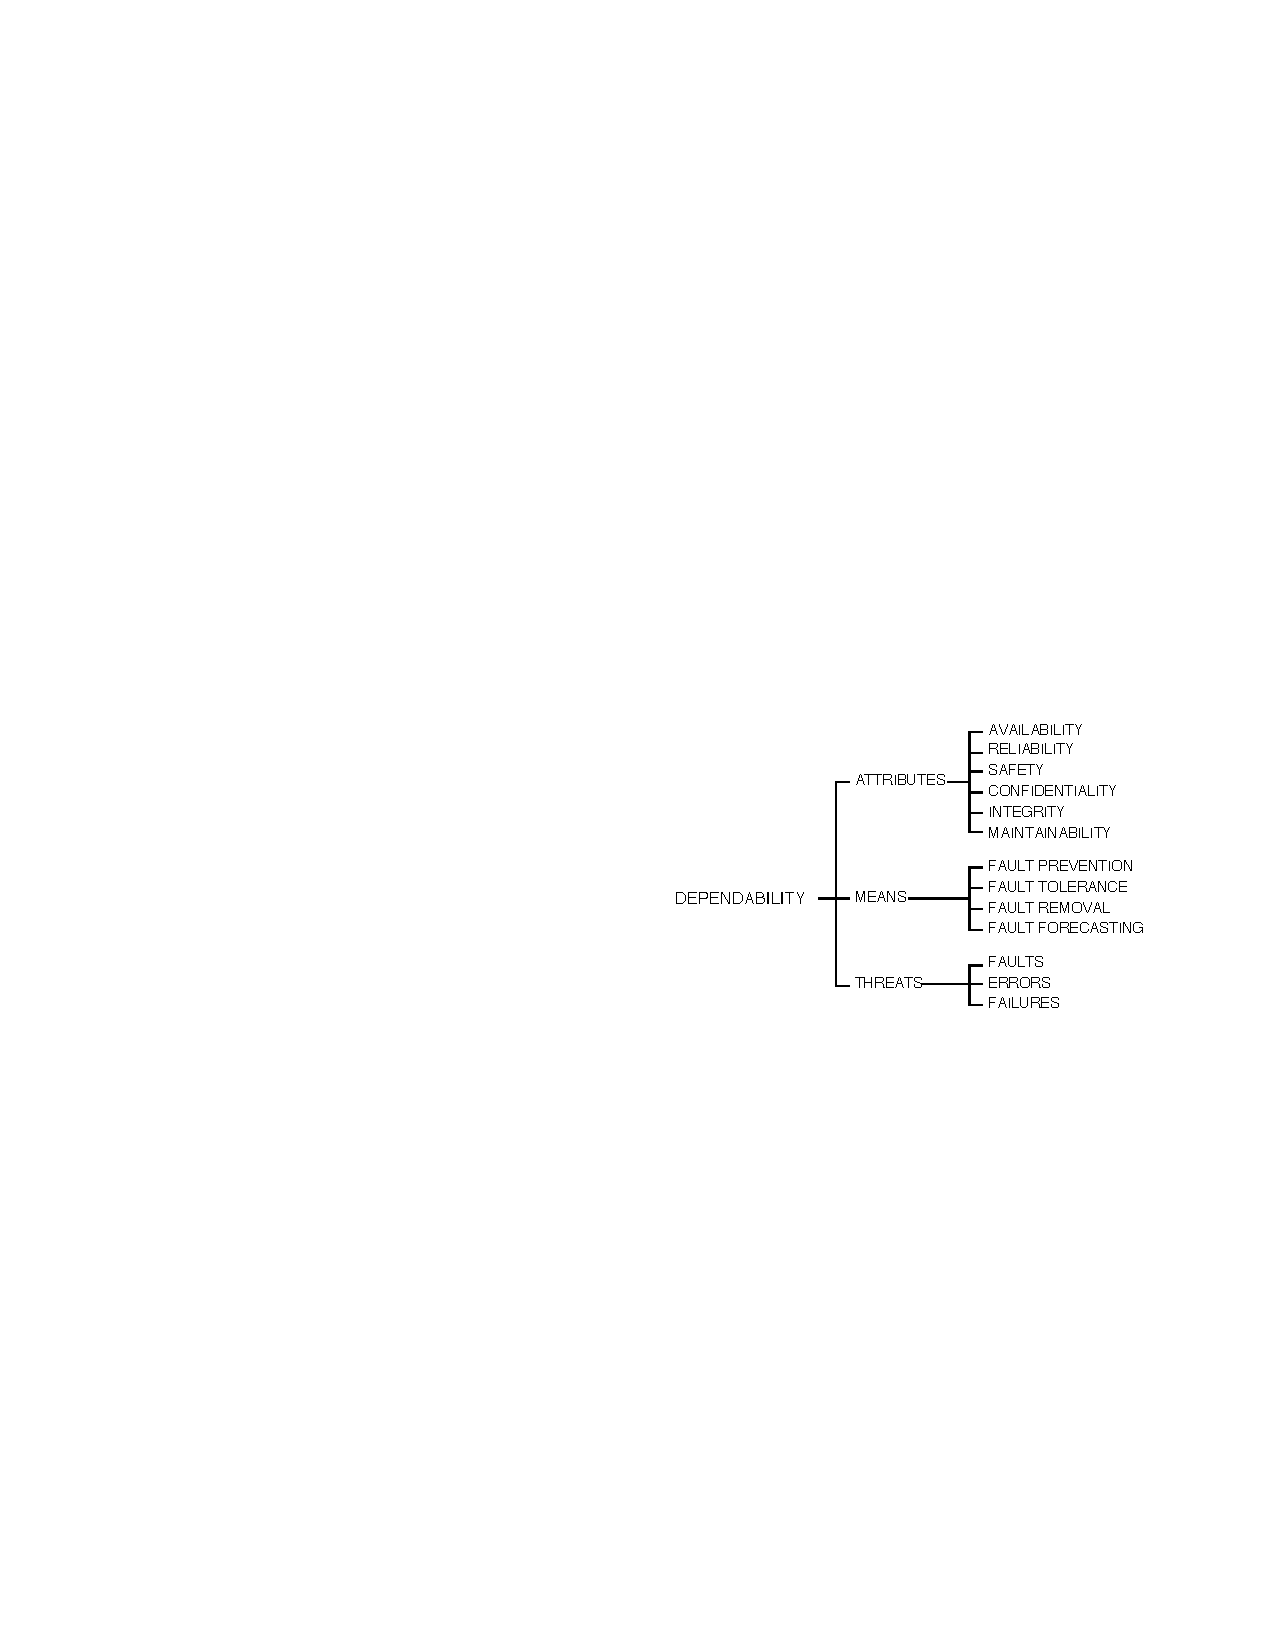
\includegraphics[width=0.8\columnwidth] {images/laprie.pdf}}
  \caption{The dependability tree by Laprie~\cite{Laprie2000}}
  \label{fig:laprie}
\end{figure}

% Goals of dependability reasoning:
%   - prediction of system failures
%   - comparison of competing designs: reason about how a change impacts dependability
%   - fullfil certification (not interesting to us)

\subsection{Dependability threats}
\label{subsec:dependability_threats}

The user has expectations over the service to be delivered by a system. These expectations may be formalized in a \emph{specification}. The delivered service can be split in two main categories: \textbf{correct} service and \textbf{incorrect} service (after Laprie~\cite{Laprie2004}). The specification may include both, even though it is more common for the specification to only include the expectations of correct service.

An example for a specification is a description of a service using the HTTP protocol~\cite{rfc2616}. The HTTP protocol specifies a request/response style message flow between a client and a server. The specification may include the location of the HTTP resources, how requests may be formed and which responses are to be expected. The specification may also include expectations for incorrect service. Each HTTP response message includes a numerical status code. If the server can not fulfill a request due to an error in itself or in its dependencies, it may use a status code equal to or higher than 500 to signify incorrect service to the client.

In the event of incorrect service being delivered, we call that a service failure, or short \textbf{failure}. The failure occurs at the moment when the user experiences incorrect service. There are different ways of how failures manifest themselves. We will reflect on some cases in \nref{ss:failure semantics}.

The reason for a failure to occur is the system being in an erroneous state, or short \textbf{error}. This means that the internal state of the system allowed a failure to occur. It is to be noted that an error is the state of the system and not an event. Only in the event of the user requesting the system's service does an error turn into a failure.

An example for an error is a server that has crashed. It is then in a state where it can not answer any client requests. The system can be in this state for a period of time, but a failure event only occurs in the moment when the client executes a request against the server.

A \textbf{fault} is the ``adjudged or hypothesized cause of an error''~\cite{Laprie1995}. Given that a fault is active, it is the cause of an error, thus there is an implication from fault to error. It is often hard to do that deduction the other way around, thus to identify the cause of an error as an exact fault. As engineers we may not be able to detect the faults themselves, but only the errors they have caused\footnote{For reference see section 3.3. in \cite{FundamentalsDepComputing}}. Therefore we use the qualifiers \emph{adjudged} and \emph{hypothesized} in the definition.

An example for a fault is a software bug which manifests itself as a single line of code and causes the server to crash when it is executed. When the software bug is in the software's codebase we call it a \emph{dormant} fault. As long as the line of code is not executed, the fault remains \emph{dormant}. It is activated the moment where the line of code is executed and then becomes an \emph{active} fault which subsequently puts the executed software into an erroneous state.

\begin{figure}[!h]
  \fbox{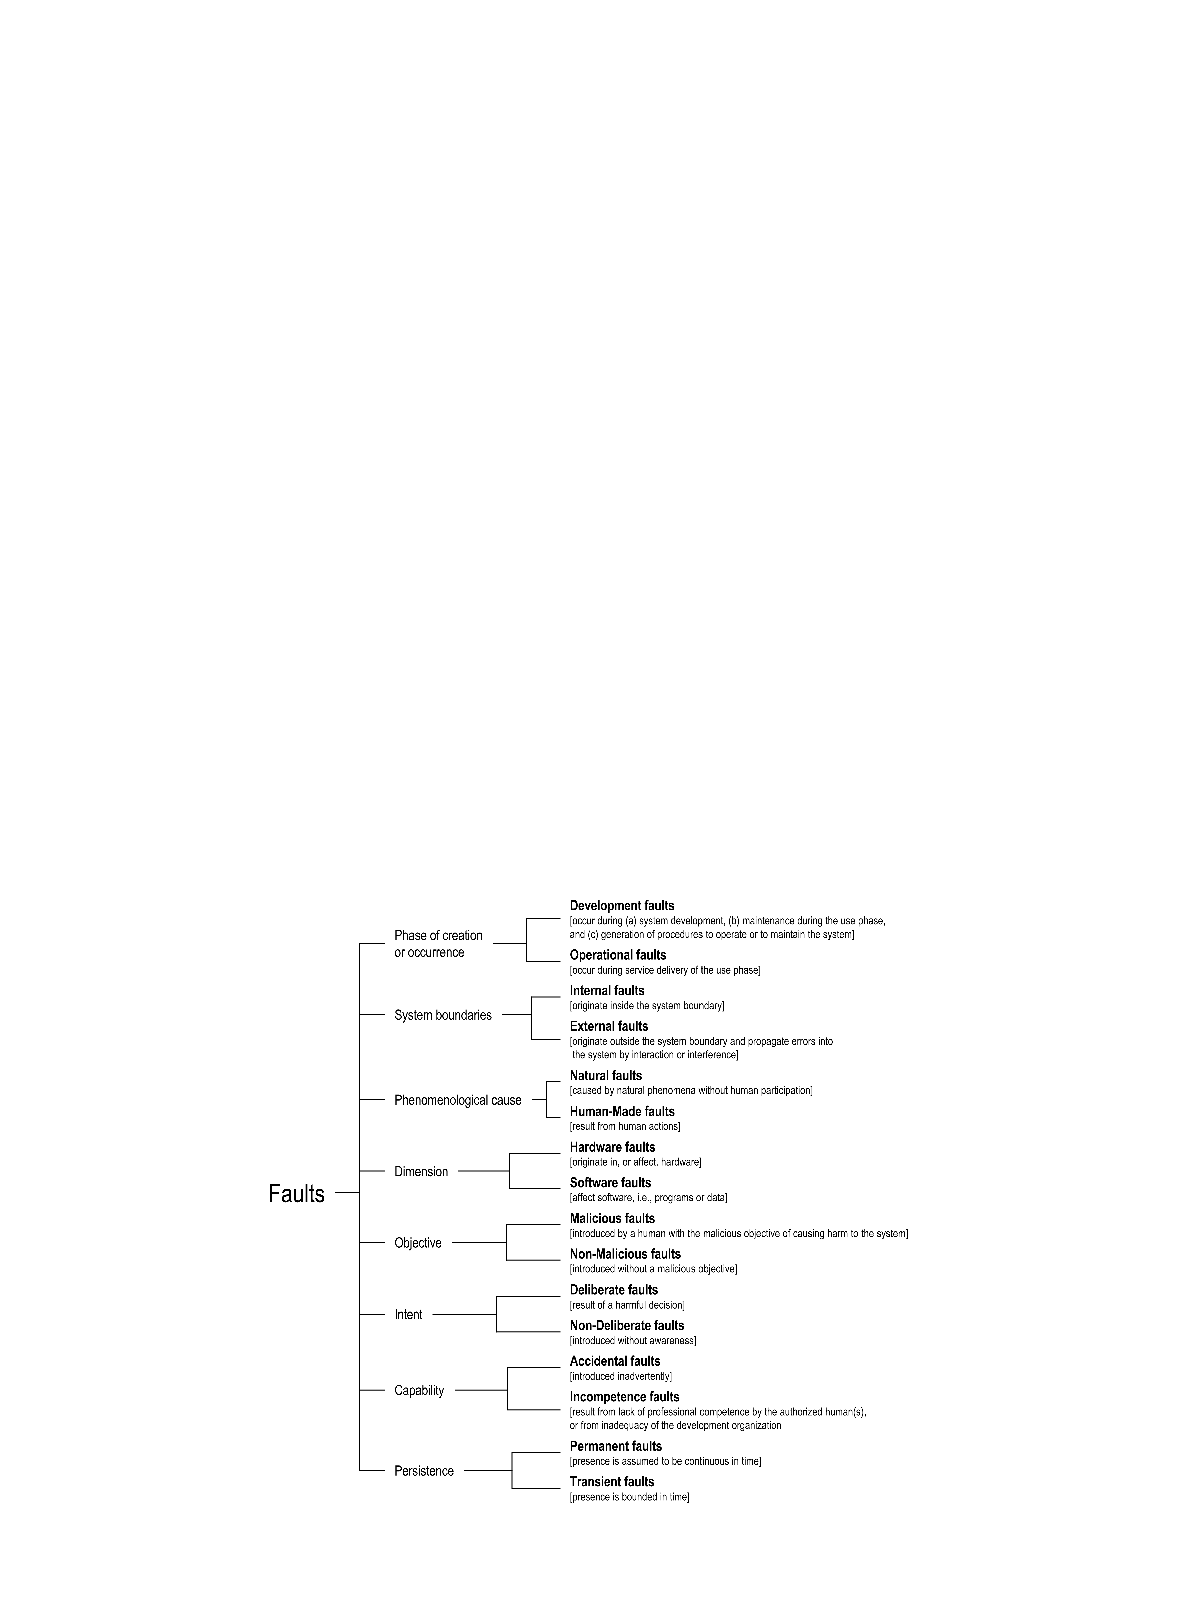
\includegraphics[width=\columnwidth] {images/faults.pdf}}
  \caption{The elementary fault classes by Laprie~\cite{Laprie2004}.}
  \label{fig:faults}
\end{figure}

Faults can be classified more precisely. Figure \ref{fig:faults} shows the elementary fault classes after Laprie. For this work, we are interested in classifying faults by \emph{system boundary}. A system boundary is defined by Laprie~\cite{Laprie2004} as ``the common frontier between the system and its environment''. The environment are all other systems that are not the system of interest. A system itself may contain other systems (usually called sub-systems or components). When classifying faults, we separate between \textbf{internal} and \textbf{external} faults.

An \emph{internal} fault originates within the system boundary. To illustrate this with an example we take a computer as a system. Internally, the computer consists of many components as sub-systems. The failure of one of the components (e.g. the memory) is a fault within the system, thus an \emph{internal} fault.

An \emph{external} fault originates from outside the system boundary. To illustrate, we again take the computer as an example. This time, we see the computer components CPU and memory as two separate systems. The CPUs correct service relies on the memory to work correctly. The failure of the memory may therefore be a fault to the CPU. Since the memory is not in the CPU, this is an \emph{external} fault to the CPU.

This hints to an interesting property, when looking at larger networks of systems that rely on each other: The failure of one system becomes the external fault of another system, which relies on it. We call this the \textbf{chain of dependability threats} (after the ``chain of threats'' by Laprie~\cite{Laprie2004}).

Figure~\ref{fig:depchain} visualizes the relation of fault-error-failure, as well as the chain of dependability threats. The arrows depict causation, from cause to effect. The boxes depict the system boundaries. \emph{System B} relies on \emph{System A}, therefore the failure of \emph{System A} may be seen as a fault in \emph{System B}.

\begin{figure}[!h]
  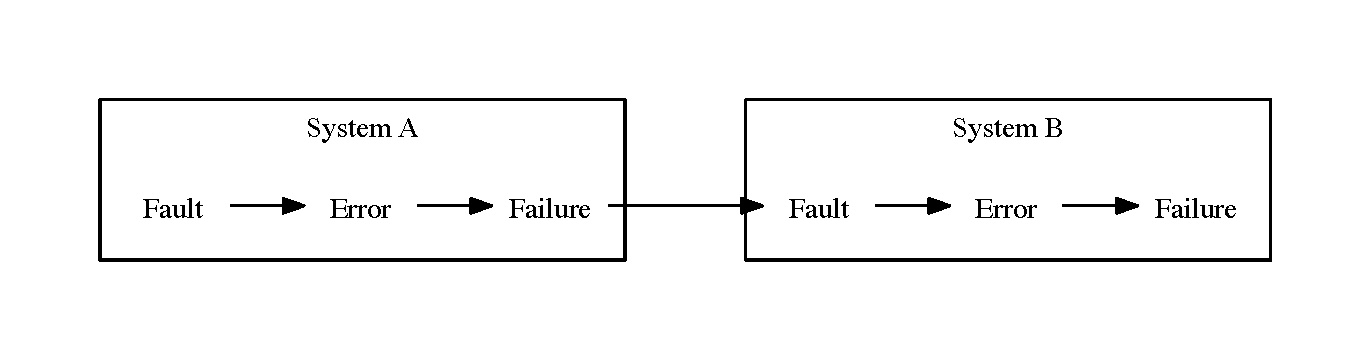
\includegraphics[width=\columnwidth] {images/chain-of-dep-threats.pdf}
  \caption{Chain of dependability threats}
  \label{fig:depchain}
\end{figure}

\subsection{Failure semantics}
\label{ss:failure semantics}

Failure semantics denote how a system and specifically its service to other systems behave in case of a fault (after Knight~\cite{FundamentalsDepComputing} section 3.8). They therefore set expectations for correct and incorrect service such that other systems may be able to guard against these.

One specific model for failure semantics was proposed by Cristian \cite{cristian}. His model is based on the notion of services (take input, execute operation, deliver output), servers who implement these services and a ``depends upon'' relation, in which the correctness of one server depends on the correctness of another server. The model then distinguishes between the following types of failures, notable within the ``depends upon'' relation:
\begin{tdescription}
  \item[Response failure] The response is incorrect. It could be in a wrong format or carry incorrect data.
  \item[Timing failure] The response happens outside of a specified time interval
  \item[Omission failure] No response is ever delivered for a request
  \item[Crash failure] After an initial omission failure all subsequent requests exhibit omission failures as well until the system is restarted
\end{tdescription}

We will build on this model later, when we propose our algorithm for constructing fault trees in \autoref{chapter:fault_trees} and explain our concrete assumptions regarding the failure semantics of the systems.

\subsection{Dependability means}
\label{subsec:dep_means}

Dependability means are ways to limit the impact of dependability threats on the dependability of a system. Following the list of means from \autoref{fig:laprie}, they include fault prevention, fault tolerance, fault removal and fault forecasting. All means focus on faults and ways to mitigate them, in order to not have them propagate to failures.

Dependability means are not in the scope of this work. For more information on this topic we recommend the work of Knight \cite{FundamentalsDepComputing}.

\subsection{Dependability attributes}
\label{sec:theory_dep_attrs}

The attributes of dependability define the different aspects, as to which the dependability of a system can be evaluated. The dependability means are there to assure these attributes against the dependability threats. In previous \autoref{fig:laprie} six attributes are mentioned. In the scope of this work we are only interested in \emph{reliability} and \emph{availability}:

\paragraph{Reliability} is defined by Laprie \cite{Laprie2004} as the ``continuity of correct service''. A more concrete definition is delivered by Knight \cite{FundamentalsDepComputing} as ``R(t) = probability that the system will operate correctly in a specified operating environment up until time t''. We assume that at the time t=0, the system was operating correctly. R(t) then denotes the probability that in the interval [0,t] the system has not suffered a failure. An underlying assumption of this reliability definition is that the system is not repairable: given that a failure occurred, the system stays in an incorrect state and may never return into a functioning correct state again.

%In the context of this work, we are concerned with software. One of the properties of software is, that it may recover from failures. This can be achieved by implementing fault tolerance mechanisms. To model this property, availability may be used.

\paragraph{Availability} is defined by Laprie \cite{Laprie2004} and Goloubeva \cite{Goloubeva2006} as ``readiness for correct service''. In contrast to reliability, availability allows for systems to be repairable after a failure occurred. Thus, a system might fail, be repaired and then deliver correct service again. During the time of repair we assume the system to deliver incorrect service.

Please note that in later \autoref{subsec:historical_availability_theory} we introduce more theoretical background, which is utilized when calculating failure probabilities from historical availability.

\subsection{Fault tree analysis}
\label{subsec:theory_faulttree}

\subsubsection{Introduction}

When we talk about dependability in systems, we eventually aim to prevent failures. For that we have to analyze the system. To do this in a structured way, many methods exist. Three notable are \emph{Failure modes, effects and criticality analysis (FMECA)}~\cite{FMEA}, \emph{Reliability block diagrams} (\cite{SysReliabilityTheory} section 3.10.), and fault tree analysis, which we will treat further in this section. All methods share the common assumption that faults happen. We may then separate faults into two categories: \emph{anticipated} faults and \emph{unanticipated} faults (\cite{SysReliabilityTheory} section 4.1). Against anticipated faults we are able to deploy dependability means. But against unanticipated faults we can by definition not defend, thus these are the most likely to propagate to failures. Therefore, one of the goals of structured methods for dependability analysis is identifying these faults as comprehensively as possible, so that they can be anticipated.

Next, we will introduce fault tree analysis further. It originated in the Bell Telephone Laboratories in 1962 for evaluating systems of the \emph{Minuteman} missile program~\cite{ericson1999fault}. It also found application in nuclear power stations~\cite{NuclearFT} and aerospace missions~\cite{NasaFT}.

\subsubsection{Definition}

A \textbf{fault tree} is defined by Rausand et al \cite{SysReliabilityTheory} as a ``logic diagram that displays the interrelationships between a potential critical event [...] in a system and the causes for this event''. Fault tree analysis is the process of constructing such a fault tree. A fault tree may be qualitative or quantitative, which we both will describe next.

\subsubsection{Qualitative fault trees}

A fault tree analysis is started by defining the system failure to investigate. We call that the \emph{TOP event} of the fault tree. From that event, all events that might contribute to its occurrence are identified as new events. They are connected to the \emph{TOP event} via the \emph{logic gates} \emph{AND-gate} or \emph{OR-gate}. This process is continued for all new events recursively, until a sufficient level of detail is reached. Thus, we acknowledge that any event can likely be seen as consisting of a more detailed fault tree, but we make the design decision for the fault tree to stop investigating this greater detail. Since the analysis method is from top down, we call it ``deductive''. The leafs of the resulting tree are called \emph{basic events}. If an event is neither \emph{basic} nor \emph{TOP} event, it is called \emph{intermediate event}.

Table \ref{tab:faulttreeelements} shows all the fault tree elements with their graphical symbols from the Fuzzed Editor~\cite{fuzzed}\footnote{All fault trees in this work were generated using the Fuzzed Editor~\cite{fuzzed} and therefore share the graphical symbols introduced here}. More elements for fault trees exist (e.g. explained in \cite{NuclearFT} and \cite{NasaFT}), but for our case the introduced elements are sufficient.

\begin{table}[!h]
  \centering
  \caption{Fault tree elements}
  \label{tab:faulttreeelements}
  \small
  \begin{tabularx}{\linewidth}{ |l|m{1.35cm}|X| }
    \hline
    Name & Symbol & Description \\
    \hline
    TOP event & 
\includegraphics[keepaspectratio=true,scale=0.8] {images/fault-tree-top-event.pdf} & The TOP event, is the event whose causes are investigated with the fault tree. A fault tree may only have one TOP event. \\
    \hline
    AND-gate & 
\includegraphics[keepaspectratio=true,scale=0.8] {images/fault-tree-and-gate.pdf} & An AND-gate connects many input events with one output event. The output event occurs only when all input events occur. \\
    \hline
    OR-gate & 
\includegraphics[keepaspectratio=true,scale=0.8] {images/fault-tree-or-gate.pdf} & An OR-gate connects many input events with one output event. The output event occurs if any of the input events occurs. \\
    \hline
    Intermediate event & 
\includegraphics[keepaspectratio=true,scale=0.8] {images/fault-tree-intermediate-event.pdf} & An intermediate event may be used as event between logic gates.\\
    \hline
    Basic event & 
\includegraphics[keepaspectratio=true,scale=0.8] {images/fault-tree-basic-event.pdf} & A basic event represents the occurrence of a specific failure event. A basic event may have a failure probability assigned.\\
    \hline
  \end{tabularx}
\end{table}

Figure~\ref{fig:fault-tree-example-qualitative} shows an example qualitative fault tree. It can be seen that there is one TOP event. ``Intermediate Event'' occurs if either ``Basic Event 2'' or ``Basic Event 3'' or both occur. ``TOP event'' occurs if ``Basic Event 1'' and ``Intermediate Event'' occur.

\begin{figure}[!h]
  \centering
  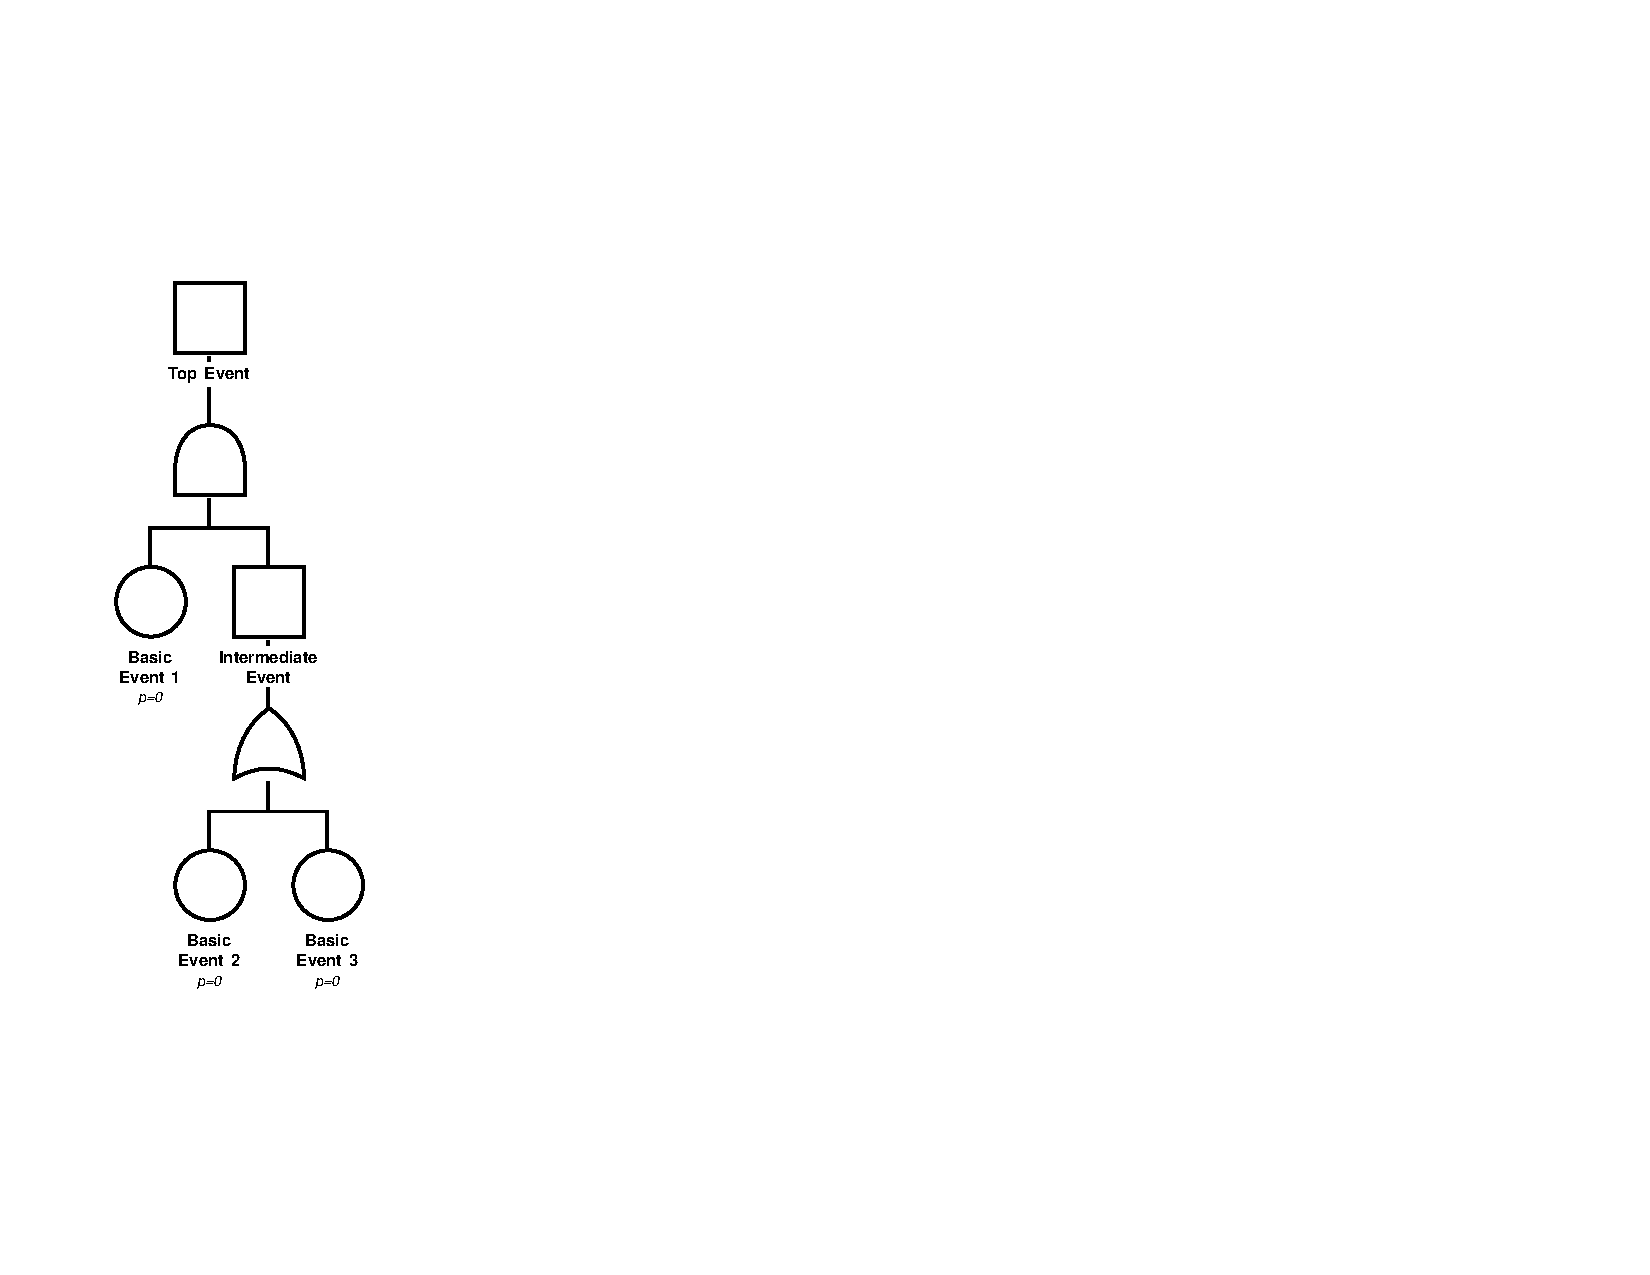
\includegraphics[width=0.25\columnwidth] {images/fault-tree-example-qualitative.pdf}
  \caption{Example qualitative fault tree}
  \label{fig:fault-tree-example-qualitative}
\end{figure}

When a qualitative fault tree exists, it may be analyzed for possible combinations of basic events that result in the TOP event (called ``cut sets'', for example explained by Rausand et al~\cite{SysReliabilityTheory} section 3.6.4.). For example this analysis then allows for the identification of single point of failures in the system.

Another value of fault trees is running the fault tree analysis itself. The analysis process involves gathering experts and addressing the problem of dependability of a system from many different viewpoints. During the process, many problems and maybe even their respective solutions may become apparent. The resulting fault tree may then be used as basis for discussion, for example to communicate the current state of the system or discuss potential changes.

\subsubsection{Quantitative fault trees}

Quantitative fault trees allow for calculating the probability of the TOP event based on the probabilities of the basic events. A quantitative fault tree analysis may use the same fault tree structure as the qualitative fault tree. Next, we will explain how such a calculation may be carried out. We base the following calculations after Limnios \cite{FaulTreesLimnios} chapter 5.

We operate under the following assumptions:
\begin{titemize}
  \item Every basic event may exist in the fault tree only once. Repeated basic events are not allowed.
  \item The basic events are independent events.
  \item The calculations are done for repairable systems.
\end{titemize}

Furthermore we assume that all basic events have a failure probability. We may now calculate the probability per logic gate: We assume A and B to be the logic gate inputs with Pr(A) and Pr(B) being their respective failure probabilities. E is the logic gate output, with the resulting failure probability Pr(E).

Equation for an AND-gate:
\[ \begin{array}{lclcl}
E & = & A \cap B & & \\
Pr(E) & = & Pr(A \cap B) & = & Pr(A) * Pr(B)
\end{array} \]

Equation for an OR-gate:
\[ \begin{array}{lclll}
E & = & A \cup B & & \\
Pr(E) & = & Pr(A \cup B) & = & Pr(A) + Pr(B) - Pr(A) * Pr(B)
\end{array} \]

Both equations may be extended for more than two inputs. To calculate the TOP event probability, we may use the ``recursive inclusion-exclusion method''~(after Limnios~\cite{FaulTreesLimnios} section 5.5.1): We start at the TOP event and resolve the immediate logic gate. We then recursively resolve all input events after the same method. Following is the equation for earlier example fault tree~\ref{fig:fault-tree-example-qualitative}:

\[ \begin{array}{lcl}
Pr(TOP Event) & = & Pr(Basic Event 1 \cap Intermediate Event) \\
 & = & Pr(Basic Event 1) * Pr(Intermediate Event) \\
 & = & Pr(Basic Event 1) * ( Pr(Basic Event 2 \cup Basic Event 3)) \\
 & = & Pr(Basic Event 1) * ( Pr(Basic Event 2) + Pr(Basic Event 3) - \\
 & & Pr(Basic Event 2) * Pr(Basic Event 3))
\end{array} \]

As we can see, the resulting equation only has probability operators and therefore the probability of the TOP event is resolvable, given that each basic event has a probability assigned.

The major value we see in creating quantitative fault trees is for comparing changes to basic event probabilities and respective impact on the TOP event probability.

  \endgroup
  %!TEX root = ../master_thesis.tex

\section{Software environment terminology}
\label{sec:software_environment_terminology}

In this chapter we propose our software environment terminology model describing the microservice architectural style. We present the individual terms and the connections between them, and reflect on some related work. Extending the architectural model, we also introduce related infrastructural systems, which are commonly utilized when realizing such an architecture.

\subsection{The microservice architectural style}

Our terminology model is similar to the field of ``Service-oriented architecture'' (short: \emph{SOA}) (e.g. described by Krafzig in \cite{enterpriseSOA} and standardized by OASIS in \cite{oasissoa}). We did not find the SOA model to be a fitting description for the microservice architectural style, which is why we propose our own model here. This chapter is not an exhaustive survey over the usage of the introduced terms, but rather sets the stage for the remainder of our work.

\subsubsection{Software architecture}

To define \emph{software architecture}, we follow the model from Fielding~\cite{Fielding}:

``A software architecture is an abstraction of the run-time elements of a software system during some phase of its operation''~\cite{Fielding}. Run-time elements are usually separated into components and connections. Since a \emph{software architecture} is an abstraction, the exact definition of what constitutes a component and a connection depends on the level of detail and purpose of the current view on the software system. For example in this work we will often use applications as the granularity level for components and application dependencies as the granularity level for connections.

``A system may be composed of many levels of abstraction and many phases of operation, each with its own software architecture''~\cite{Fielding}. The different levels manifest themselves most prominently in the fact that each component in an architecture may consist of another architecture in itself. Continuing with the example from above, one application might in itself have an architecture consisting of its deployed services, or how its internal code modules relate to each other. The phases of operation may be seen as changing over time (for example the architecture changed between an hour ago and now) or states (for example the architecture changed when a new application was introduced).

\subsubsection{Software architecture style}

\emph{Software architecture styles} try to categorize common aspects of \emph{software architectures}. These aspects might be similar patterns in structural organization, the same granularity of components and connectors or similar constraints on how these work together as one system \cite{Shaw1996} \cite{fowler-microservices}.

\subsubsection{Software as a Service}

\emph{Software as a Service} (SaaS) is a software delivery model, in which the software code, computing resources and user data are managed by a provider. The software is remotely accessed by the consumer via a thin client, most commonly a web browser \cite{Carraro}.

Traditional software delivery models involved shipping executable software to the users, who then operated them on their own computing resources \cite{swebok}. Since SaaS software is operated by the vendor, it is possible to release software at a higher rate, sometimes several times in a day \cite{etsydeploy} \cite{ContinuousDelivery}.

In this work, we are concerned with multi-user SaaS, thus all users use the same computing resources supplied by the vendor, they have the same service level agreements and limited customization options \cite{salesforce} \cite{Mietzner2009} \cite{Azeez2010}. One promising architectural style for building a multi-user SaaS is the \emph{microservice architecture style}, which we will introduce next.

% The following definition is given in \cite{zhangsaas}: ``[...] the SaaS delivery model essentially separates software ownership from the user—the owner is a vendor who hosts the software and lets the user execute it on-demand through some form of client-side architecture via the Internet or an intranet. This new model delivers software as utility services and charges on a per-use basis [...]''

% In  the authors define SaaS as ``software deployed as a hosted service and accessed over the Internet" and further define it technically as ``the SaaS provider hosts the application and data centrally—deploying patches and upgrades to the application transparently, and delivering access to end users over the Internet through a browser or smart-client application''.

\subsubsection{Microservice architectural style}
\label{subsec:microservice_architecture}

% \definition{A services architecture is a software architecture style consisting of applications that interact with each other through services.}

Fowler et al \cite{fowler-microservices} define the \emph{microservice architecture style} as ``an approach to developing a single application as a suite of small services, each running in its own process and communicating with lightweight mechanisms, often an HTTP resource API''. In our case, the ``single application'' is the \emph{SaaS} as experienced by the user.

\emph{Microservice architecture} shares concepts with the ``Service-oriented architecture'' (SOA) style, but we decided to not use the term SOA directly due to the ambiguity of its meaning (as described by Fowler et al \cite{FowlerSOAAmbiguity} and Partridge et al \cite{modServicesAnalysis}).

The terms following next are all to be seen in the context of microservice architecture, and therefore define it further.

\subsubsection{Application}
\label{ss:application}

\begin{figure}[h!]
  \caption{Entity-relationship model of the terms defined in this chapter}
  \label{fig:software-env-erm}
  \makebox[\textwidth][c]{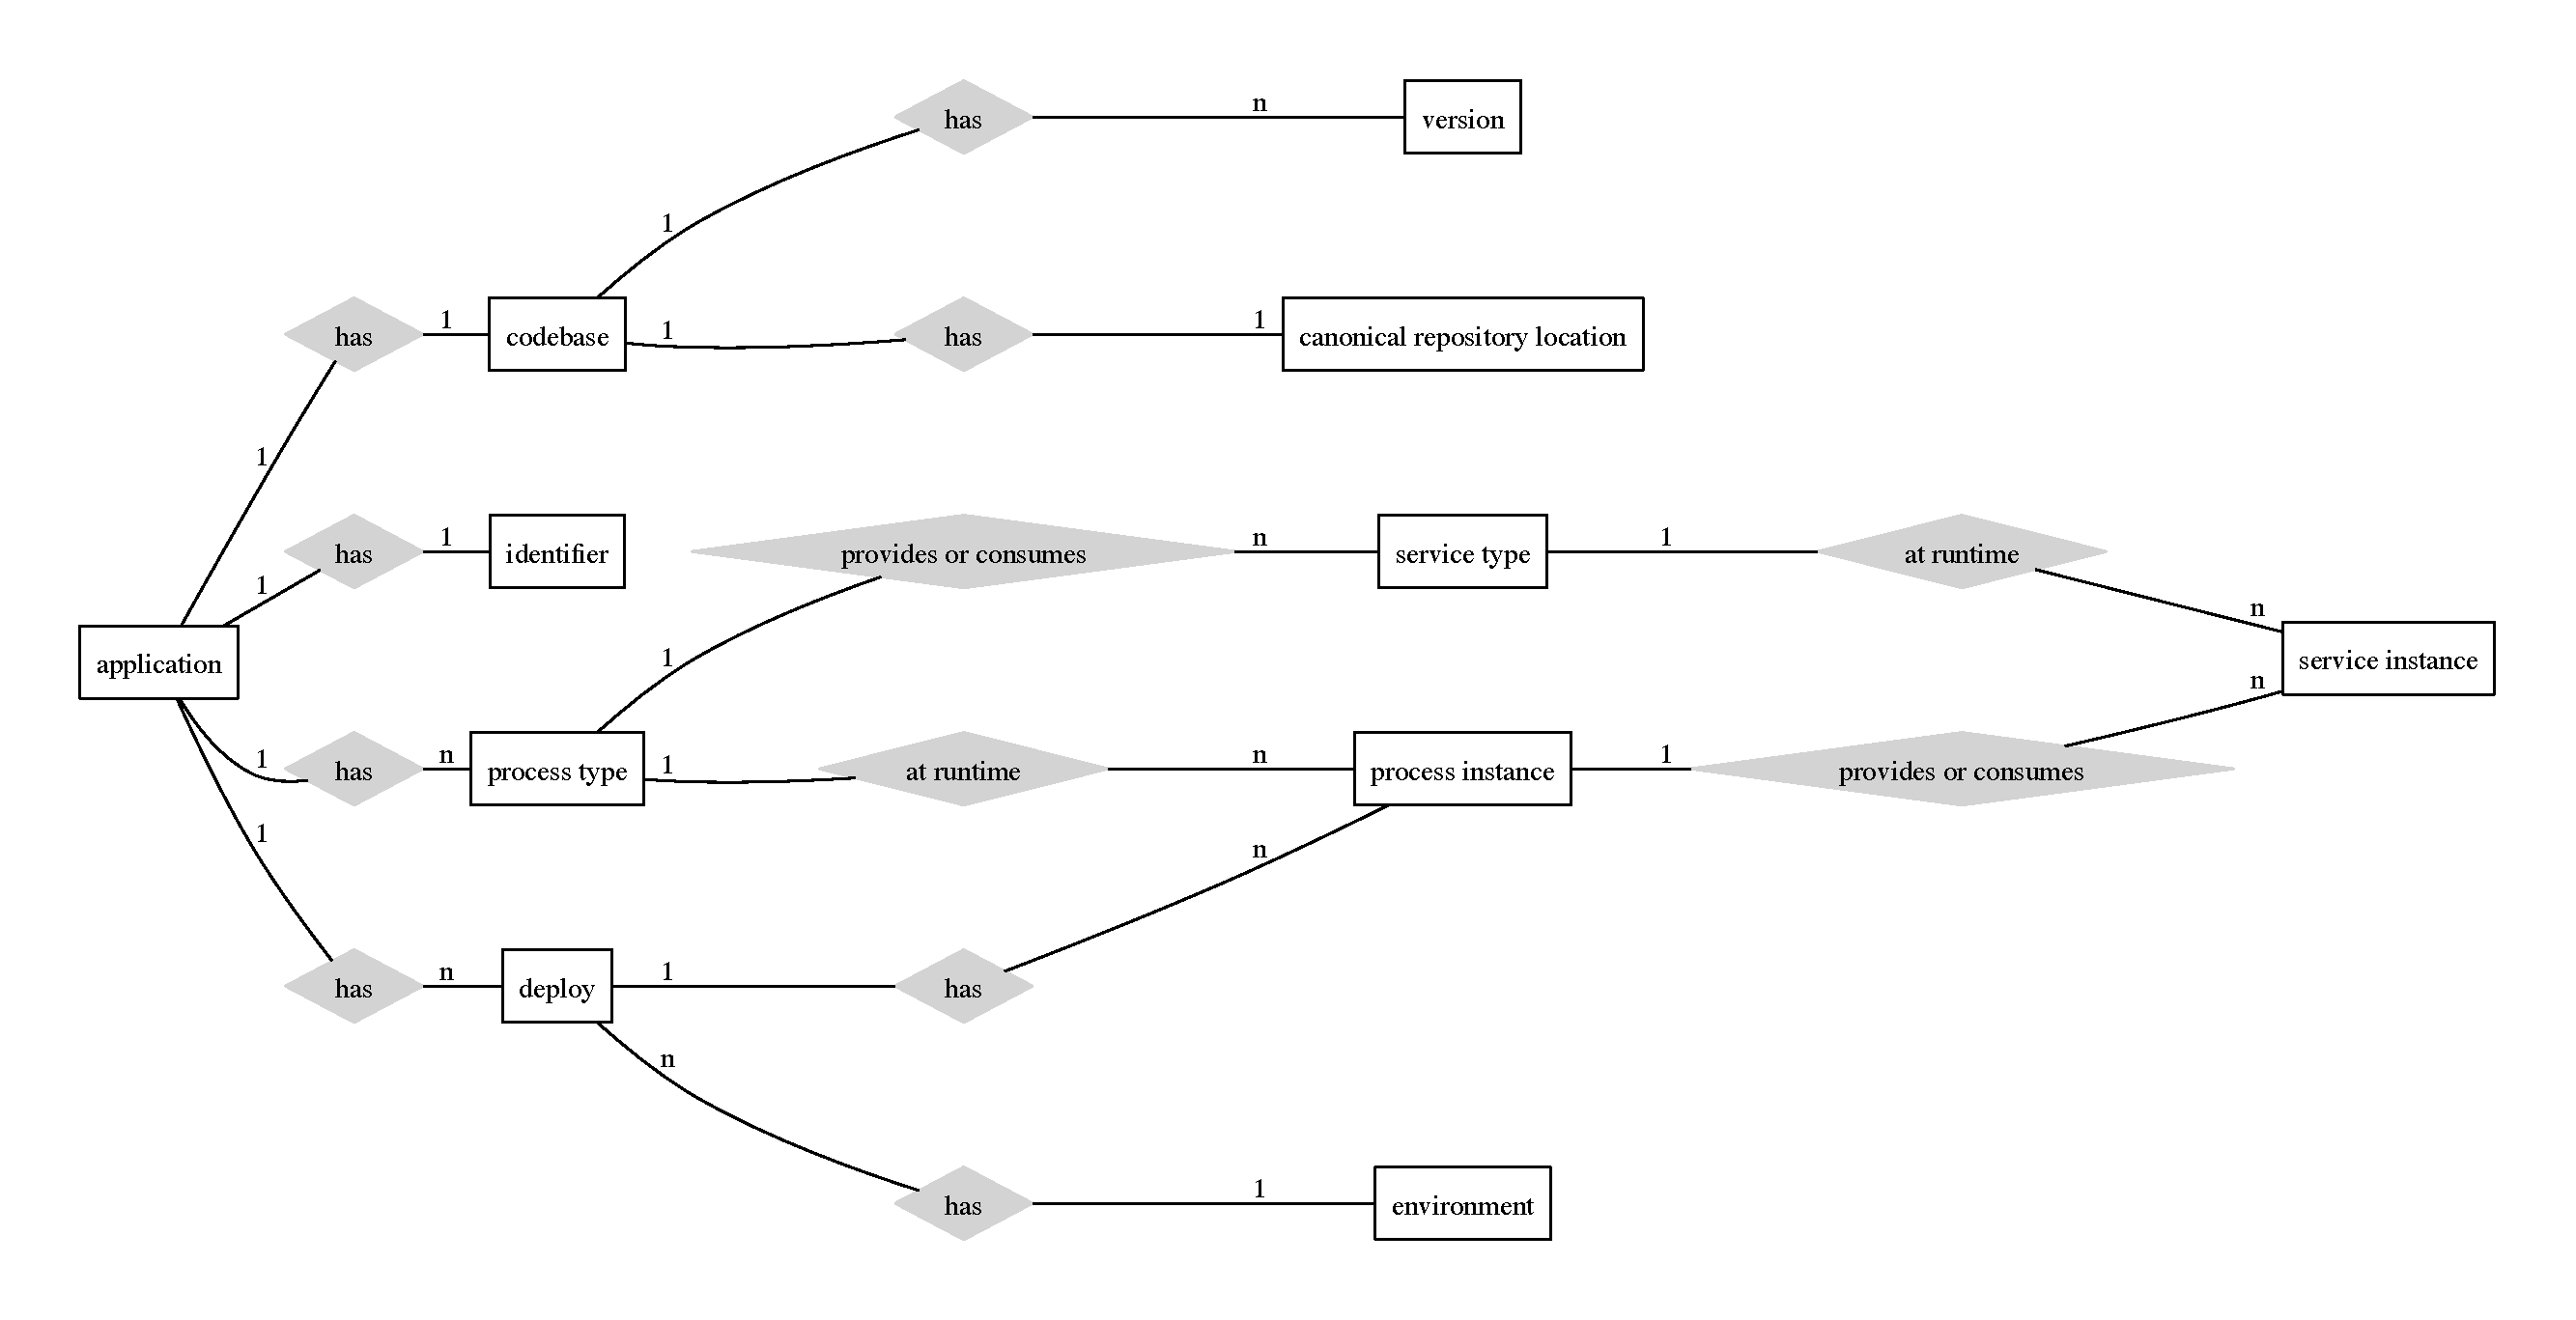
\includegraphics[width=1.15\linewidth] {images/env.pdf}}
\end{figure}

An \emph{application} is the implementation of capabilities. Capabilities manifest themselves as having a real-world effect \cite{modServicesAnalysis}. Usually the users of an application are able to observe its real-world effects during operation.

The following technical descriptions of \emph{applications} are related to the observations made by Wiggins~\cite{12factor} as part of ``12 factor applications'', but have been customized by us as core part of the terminology model, especially regarding the interrelation to other concepts. We visualize the interrelation of the described concepts in \autoref{fig:software-env-erm}.

Every application has exactly one \emph{codebase}. The codebase may consist of files that are required to execute the application (e.g. source code) as well as meta data (e.g. documentation). The codebase is tracked in a source code version control system like Git~\cite{ProGit} or Subversion~\cite{svn}. We assume that within that system there is a canonical location for the codebase repository. Within that repository, the codebase might exist in different versions. We assume that for every repository, there is always a canonical version that represents the current state of development.

When an application is executed at runtime, its concrete representation are \emph{processes}. One application may have many process types, each of which may have many process instances at runtime. We explain processes further below.

Every application has at least one identifier, which is unique in the current scope of investigation, which in our cases here is the organizational boundary of the company.
% We follow the definition in \cite{rfc3986}: ``An identifier embodies the information required to distinguish what is being identified from all other things within its scope of identification.". How the identifier is actually structured is less important for our works, but possibilities would be the ``Uniform Resource Identifier'' from \cite{rfc3986} or following the structure of the ``host'' component as defined in the same document.

We distinguish between \emph{internal} and \emph{external} applications, based on the boundaries of an organization. The development of an \emph{internal} application is driven within the organization. The development of an \emph{external} application is driven externally to the organization. We assume both application types to be executed within the organization, thus on the machines under the control of the organization. An \emph{external} application may also be executed outside of the organization if specified (e.g. services provided by other SaaS platforms).

Another categorization of applications we propose is between \emph{client-facing} and \emph{infrastructure} applications:
\begin{tdescription}
  \item[Client-facing applications] serve a \emph{client-facing} functionality. Thus, if such an application would be removed, the clients (and the human users of these) would notice a lack of functionality. Often these applications are very specific to the business they support.
  \item[Infrastructure applications] support the \emph{client-facing} applications in their operation, but in themselves do not provide a client-facing functionality. Thus, if the infrastructure application would be removed, the clients (or human users of these) would not notice a lack of functionality (given that the \emph{client-facing} applications were still able to operate). We will discuss infrastructure applications further in the following \nref{subsec:infrastructure}.
\end{tdescription}

In our work, we focus on \emph{client-facing} applications. Forth going when we talk about ``applications'', we implicitly exclude \emph{infrastructure} applications.

An application may have many \emph{deploys}, as explained next.

\subsubsection{Deploy}

A \emph{deploy} of an application consists of the application's process instances executed in a specific environment. It may also be referred to as an application at runtime. But since an application itself is an abstract entity, the concrete representation of it at runtime are its processes instances.

Every deploy is executed within a specific environment. Common names for such environments are ``production'' or ``staging''. For each environment, a deploy might be configured differently, for example with regards to runtime parameters like queue lengths and timeout thresholds, or the location of services to consume.

The deployment of an application is often facilitated by deployment systems, which we introduce later in \nref{subsec:deploymentsys}.

\subsubsection{Process}

A \emph{process} is the concrete representations of an application at runtime. One process always belongs to one application. One application may have many processes. A process may be seen from two viewpoints: as process instance and as process type.

A \emph{process instance} exists during execution, where it might use resources like CPU time, memory, files or I/O devices. The implementation details of how a process instance is managed during runtime is not of interest for our work, but we assume that its resources and lifecycle are managed by an operating system, for example as described by Silberschatz et al \cite{silberschatz1998operating}.

A \emph{process type} is a logical entity embodying the opportunity to execute process instances of it. A process type usually manifests itself in some way in the source code of an application, for example by being a dedicated software module.

Every process instance always has exactly one process type and one deploy, whereas a process type may have many process instances, which in may even belong to different deploys. When we speak of ``a process'' it embodies both concepts of \emph{process instance} and \emph{process type}, which may be used interchangeably depending on the current context of discussion.

A process may consume and provide many services, as explained next.

% An application might implement services, which might then be consumed by other applications. Vice versa it might also consume services, provided by other applications. If an application does neither provide nor consume a service, then it is not interesting in the investigations of this work.

\subsubsection{Service}

A \emph{service} provides access to the capabilities of an application to other applications via a network. The possible ways of access are defined through a service interface. A service interface might be standardized in a machine-readable format like a WSDL definition~\cite{wsw3c}, or just be defined through the implementation itself.

Services are implemented as processes. Just as with processes, we may speak about service types and service instances. Since each service may be consumable via a network, a service also needs to be addressable. Therefore each service instance may have a URI, via which it may be consumed by other processes.

If a process exposes its functionality via a service interface, it provides a service. If a process starts a connection to a service, it consumes that service.

% Contrary to definitions of services in ``web services'' \cite{w3carch} \cite{w3cwsa} as well as ``SOA'' \cite{enterpriseSOA}, we do not assume that services have machine-readable service interface descriptions. We also do not

The access to services is facilitated as machine-to-machine interaction over a network, as described next.

\subsubsection{Service communication}

\emph{Service communication} happens between a service consumer and a service via a network connection, over which they may exchange messages.

We assume that service consumer and service are interoperable over an agreed protocol stack which should adhere to the standards set by the Internet protocol suite \cite{internetprotocol}.

We do not assume anything on the communication pattern. Examples might be request-response \cite{requestresponse} or publish-subscribe \cite{publishsubscribe}. The service provider is always the process that accepts the connection. The service consumer is the process that established the connection.

We do not assume anything on the locality of the service and the service consumer. They might be on the same physical machine, in different datacenters, or within different organizations.

% An application may implement many services. It is then called a service provider. It may also be called a server, following the definition in \cite{rfc2616}: `` An application program that accepts connections''.
%
% An application that consumes services is called a service consumer. It may also be called a client, following the definition in \cite{rfc2616}: ``A program that establishes connections''.

\subsubsection{Service dependency}
\label{subsec:service_depenedency}

A \emph{service dependency} is the fact that a process is the consumer of a service. The service dependency is always directed from service consumer to service provider.

Given that a service dependency exists, it may also be noted with the related applications (as either service dependency or application dependency).

Please note that a service dependency is not to be confused with a shared library dependency: Both concepts have in common that the dependency is to another software component. These components are often developed in a different organizational context than the program that depends on it. This manifests itself in decoupled software life cycles. The difference between both concepts is that a shared library dependency is executed in the same context as the program (e.g. the same process) and usually used via an in-memory function call. On the other hand, a service dependency is executed in another context (e.g. another process, machine or datacenter) and therefore the communication may not happen via in-memory function calls, but through mechanisms like remote procedure calls \cite{Birrell1984} or web services \cite{wsw3c}.

\subsubsection{Machines}

A \emph{machine} consists of a CPU, memory, permanent storage and an operating system. Every machines is connect to a network and may be addressable and accessible over it. A machine might be physical or virtual, but is always under the full control of the organization. A machine provides the execution context for processes and might be used by \emph{client-facing} and \emph{infrastructure} applications alike.

\subsection{Infrastructure systems}
\label{subsec:infrastructure}

When building a microservice architecture, certain types of systems are commonly used to support its realization. We call these \emph{infrastructure system}, since they form the infrastructure for developers to build \emph{client-facing} applications on. In this section we will describe three types of infrastructure systems: \emph{deployment}, \emph{service discovery} and \emph{telemetry} systems. We introduce their concepts here and will describe the concrete implementations we found for them in our case study in later \nref{chapter:case_study}.

\subsubsection{Deployment systems}

For an application to be actually used at runtime, it needs to be deployed. A deployment procedure usually starts with the application's codebase and ends with process instances running.

The foundation for each deployment system is that there are available computing resources under control of the organization. The deployment system then matches available resources with processes of application deploys and cares for starting the process instances. This might include building the application, distributing the build artifacts to the correct machines, setting up the runtime and configuration environment as well as starting and supervising the processes at runtime. This implies that the deployment system has knowledge about existing applications and about currently running process instances.

It is possible to execute a deployment procedure manually without utilizing a dedicated deployment system. Engineering experience has shown that it is desirable to automate deployment procedures as much as possible in order to increase development speed and lower potential for failure. Humble et al \cite{ContinuousDelivery} motivate and describe this subject in detail.

\subsubsection{Service discovery}

When a process wants to consume the service of a certain application or deploy, it has to know the service's location. Service discovery answers this question, mapping an application name (and possible more qualifying information like deployment environment or datacenter) to the location of the services. Listing \ref{list:sd_example} shows an example of such a mapping. Since a deploy might have many process and service instances, service discovery might return the locations of all of these. Since we assume all service communication to happen via the TCP/IP protocol stack, the eventual format of a service locations is always an IP address and a port number.

\begin{lstlisting}[language=json,numbers=none,caption=Example for a service discovery mapping from service discovery key to service locations with IP address and port number,label=list:sd_example,backgroundcolor=\color{white}]
"myapplication" -> [ "10.20.30.1:123", "10.20.30.2:321"]
\end{lstlisting}

% Difference in how changes are propagated:
%
% Might be pull: client has to pull from source of service discovery, what the current configuration is
%
% Might be push: once the service discovery configration changes, it pushes these changes to all to all clients
%
% Might be tiered: initial entry point is pulled (and might also only be done once then), but from there service discovery is done on each call by another entity. Cases are load balancer (must now how to reach load balancer, from there load balancer knows all backends) or via message bus (must know location of message bus, message bus distributes to all recipients).

\subsubsection{Telemetry}

Telemetry is defined in \cite{merriamwebstertelemetry} as ``the process of using special equipment to take measurements of something (such as pressure, speed, or temperature) and send them by radio to another place''. Telemetry systems are the basis for reasoning about the current state of the system, since they collect measurements and present them to engineers in a queryable format. Telemetry systems are also used for setting up alerting. Since in a microservice architecture process instances are by definition distributed over many machines, a dedicated telemetry system is needed for effectively providing engineers with the relevant information about the systems state.

\section{Summary}

In this chapter, we first introduced aspects of dependability theory based on the ``dependability tree'' by Laprie (visible in \autoref{fig:laprie}). We described the dependability threats \emph{fault}, \emph{error} and \emph{failure} and how these relate to each other. Based on the categorization of faults into \emph{internal} and \emph{external} faults, we mentioned the \emph{chain of dependability threats} as a model to understand propagation of failures between interdependent systems. As attributes to qualify dependability we described \emph{reliability} and \emph{availability}. Afterwards we introduced qualitative and quantitative \emph{fault trees} as ways to model dependability.

To describe the microservice architectural style further we proposed an own terminology model. At the core it defines what an \emph{application} is and how applications may depend on each other through services. The interrelation of the introduced terms can be seen in \autoref{fig:software-env-erm}. We ended the chapter by introducing infrastructure systems that support the realization of microservice architectures.
  %!TEX root = ../master_thesis.tex

\chapter{Case study}
\label{chapter:case_study}

In this chapter we describe the case study and explain how the terminology model we proposed in previous \nref{sec:software_environment_terminology} relates to it. We re-state our problem in the context of the case study, highlight the evolution of architecture in the case study and introduce the concrete implementations of infrastructure systems, which are relevant to our work in later chapters.

In the first quarter of 2014, the author worked with SoundCloud~\cite{soundcloud} in the context of this work. SoundCloud produces one product, which they describe as ``the world’s leading social sound platform where anyone can create sounds and share them everywhere''~\cite{soundcloudabout}. In October 2013 it had 250 million monthly active listeners \cite{soundcloudusers}. On May 9th 2014, the Alexa Global Rank of the product was 166 \cite{alexasoundcloud}. In April 2013, the company had 190 employees in four offices (Berlin, London, San Francisco, Sofia) with 80 engineers mainly located in the Berlin office~\cite{soundcloudAG}.

In the deployed microservice architecture of the case study we found hundreds of applications and thousand of processes deployed in the productive environment.
One of the problems that became apparent to us while interviewing engineers as well as through observing the day-to-day work in the company was that there did not exist a holistic understanding of how applications and processes relate to each other. Often not even the immediate dependencies of applications were clear to engineers, manifesting themselves in the two questions ``Which applications does my application depend on?'' and ``Which applications depend on my application?''. Resulting from these observations, we especially found the question of how failures propagate through the system to be an interesting angle for research.

Before we discuss our solutions to these problems in the following chapters, we will discuss the technical environment of the case study more closely.

% A note of caution: The nature of development in our case study was optimized for high velocity, which means that systems might change rapidly. Therefore the information we present here is a snapshot and is likely to have changed already again by the release of this works.

\section{Architectural style}
\label{sec:architecture}

We separate the product into two big categories: \emph{clients} and the \emph{platform}. The clients are software that is executed within the realm of the human users. This software may be the website on \emph{soundcloud.com} running in a web browser, native applications (mostly on mobile devices) or consumers of the public REST API~\cite{soundclouddevelopers}~\cite{Fielding}. The client software may be developed by the company or by third parties. All clients interact with the platform via APIs based on the HTTP protocol~\cite{rfc2616}. Usually the clients functionality is tightly bound to the functionality provided by the platform. In fact they might provide no functionality at all if there is no connectivity to the platform. Clients are not the focus of this work and will not be represented in further investigations. This is based on the notion that due to the context of the execution of clients we do not see them as part of the microservice architecture, even though they technically consume services provided by the microservice architecture. Figure \ref{fig:evolution_example} shows how clients and platform relate to each other.

The \emph{platform} is implemented as a \emph{multi-user} \emph{Software as a Service}. Thus, the software, the runtime resources and the user data are managed by the company. The platform is implemented as \emph{multi-user}, meaning that all users use the same computing and data storage resources.

The development of the platform started in 2007. Since then, it has been incrementally developed further in evolutionary steps, which we will describe next:
\begin{tdescription}
  \item[1. Monolithic application] Initially, the platform development started with the \emph{Ruby on Rails}~\cite{Rails} web development framework. All presentation and business logic was concentrated in one monolithic application, which was executed with one process type and many process instances. One database system held all data.
  \item[2. Splitting the monolithic application] Starting 2010, functionality started to be moved out of the monolithic application and into independent applications \cite{Phil2013Monolith} \cite{EvolutionTreadway}. These applications might still have major functional dependencies on the business logic of the monolithic application. New features are not developed in the monolithic application anymore, but as new applications. We see the case study being currently in this stage, since the monolith still carries major significance.
  \item[3. Full microservice architecture] The goal of the architecture evolution is to reduce the significance of the monolith to ``just being another service''. Thus, the functionalities of the platform as a whole should be split relatively equally over all applications. A platform that is developed further towards this style is Twitter, introduced in \cite{twittersoa}.
\end{tdescription}

Figure \ref{fig:evolution_example} visualizes these three evolution steps.

\begin{figure}[h!]
  \centering
  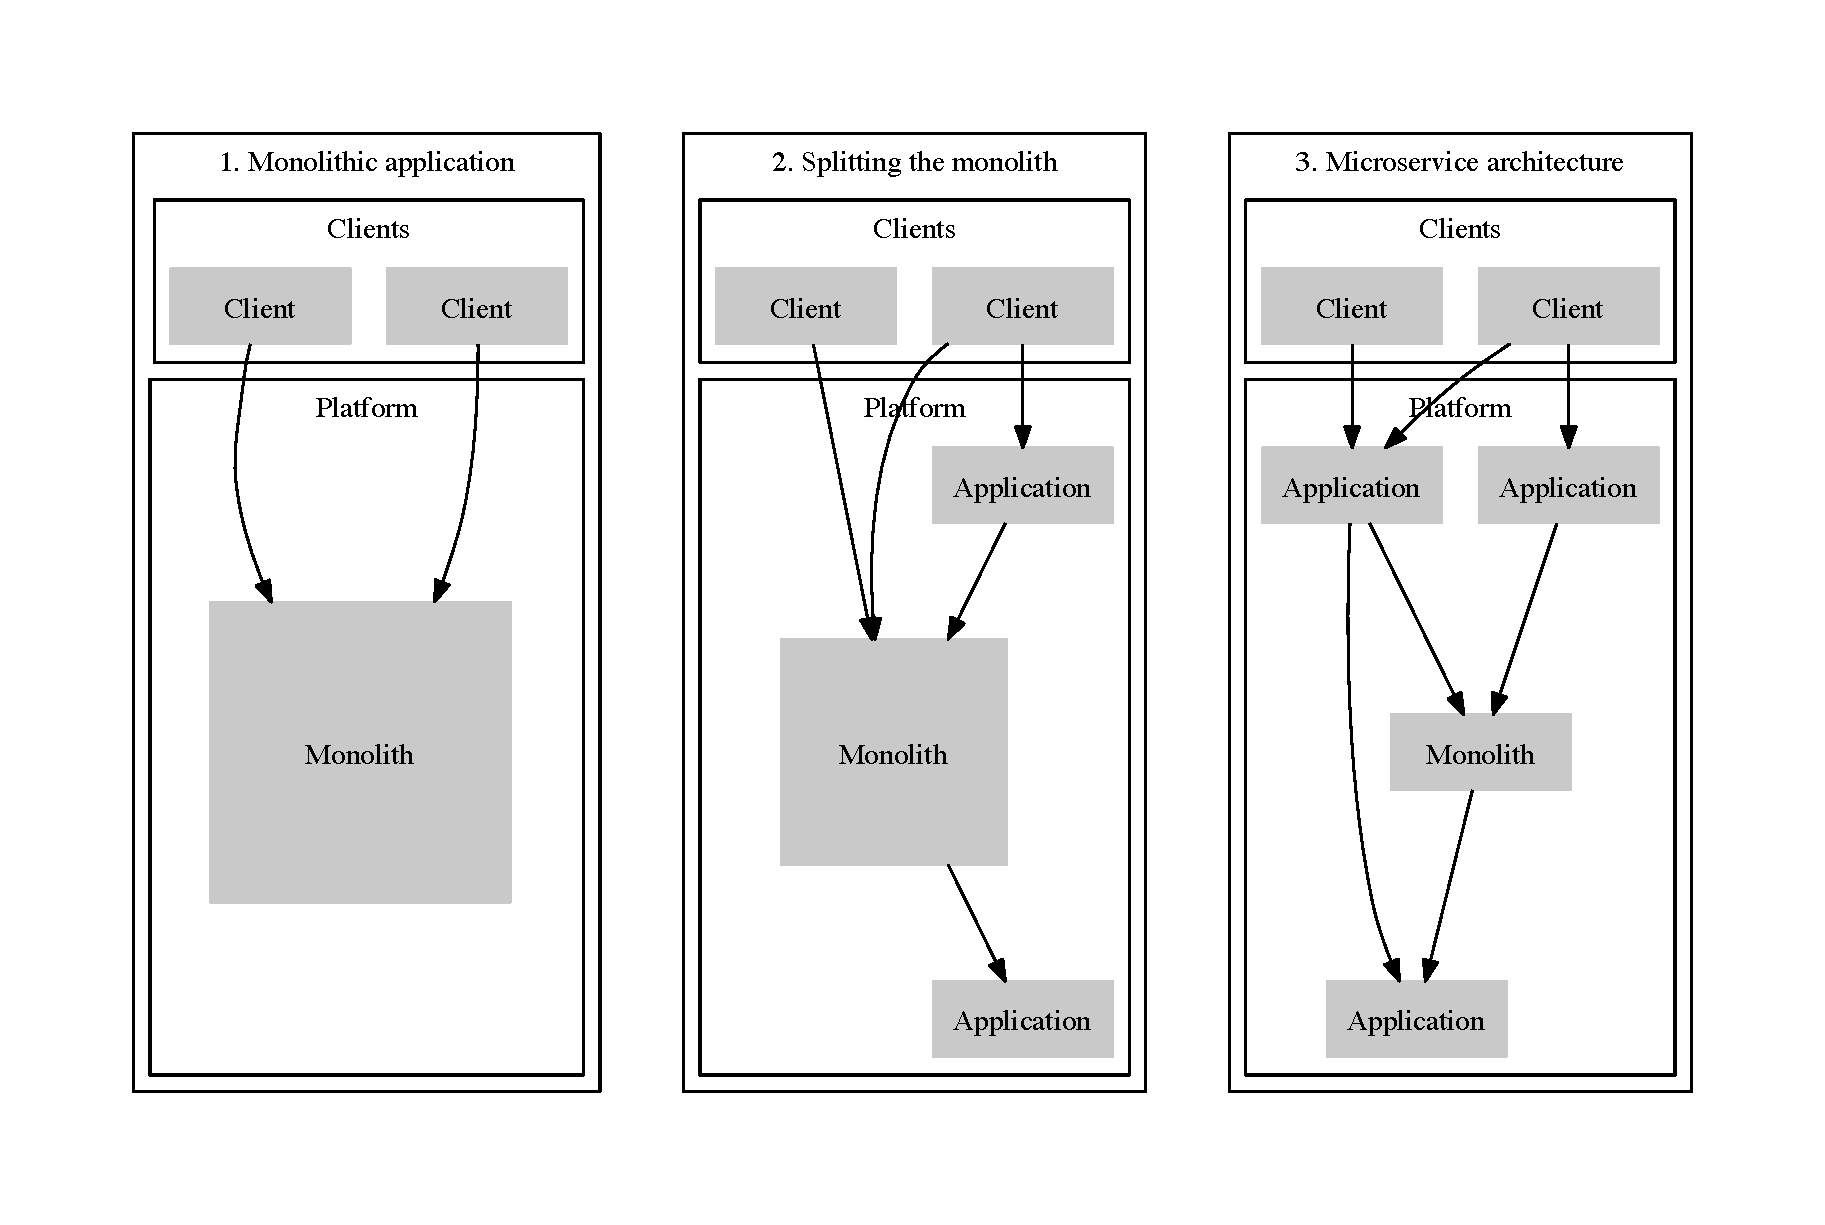
\includegraphics[width=\linewidth] {images/arch-evolution.pdf}
  \caption{Visualization of the architecture style evolution from monolithic architecture style to microservice architecture style. Boxes represent applications and directed edges represent service dependencies. Size of the ``monolith'' represents its significance in the architecture.}
  \label{fig:evolution_example}
\end{figure}

We see two major drivers for this evolution:
\begin{tdescription}
  \item["The right tool for the job"] Different functionalities require different approaches to implement them efficiently. These approaches may be hard to consolidate in one application, most notably since different programming languages or frameworks might be used.
  \item[De-coupling of development and deployment] Small teams of 2 - 10 people are believed to work more effectively than bigger teams \cite{HenrikKniberg}. Conway's law~\cite{conway} suggests that the structure of a system designed by an organization will follow the organization's communication structure. Following this law, it is logical to assume that as an engineering organization grows with many small teams, the architecture will follow the same style. As a side benefit, small teams and applications allow for easier and therefore more often application deployment, which in turn increases the velocity and quality of software \cite{fowler-microservices} \cite{ContinuousDelivery}.
\end{tdescription}

During our investigations we noted that the development of the architecture was not centrally controlled but rather happened to the discretion of individual engineers. Every engineer was able to decide how functionalities should be split into different applications. This led to a lack of oversight over the architecture development in the engineering organization. During our investigations we also found many different technologies in use for developing applications. For example we found 9 different programming languages used in the case study (as further explained in \nref{subsec:from_smi}, especially Table \ref{tab:SIM_language_stats}).

\subsection{Technical details}
\label{subsec:case_study_tech_details}

In this section we cover some technical details of the case study.

All codebases were organized with the Git~\cite{ProGit} source code versioning system. The canonical location for all repositories is at GitHub~\cite{github}, which is a SaaS providing Git repository hosting.
In our case study, all repositories were organized within one ``GitHub organization''~\cite{ghorgs}, which is a logical grouping of hosted repositories, providing centralized access control and billing. We provide more statistics over repositories and their usage in later  \nref{subsec:graph_manual_annotation}.

All repositories on Github have an identifier. Since each application has a canonical Github repository and since these are unique, we may use the repository identifiers as application identifiers as well. We found two cases where a repository contained several applications. In these cases we assigned that repository to several applications with different identifiers\footnote{One of the cases is described later in \autoref{sec:case_study_execution}}.

% \subsubsection{Inter-process communication}
%
% In our case study, all inter-process communication happens
%
% Network communication is the way for inter-process communication in the case study. The internet protocol suite (most notably TCP/IP~\cite{internetprotocol}) was the common basis for network communication. As application layer protocol HTTP~\cite{rfc2616} was the most commonly used.

In our case study, machines were distributed over several company-operated datacenters as well as rented cloud platforms. Several different Linux distributions were in use.

\section{Infrastructure systems}

Next we will describe the systems for \emph{deployment}, \emph{service discovery} and \emph{telemetry} that we found in our case study.

\subsection{Deployment systems}
\label{subsec:deploymentsys}

In our case study we found various systems facilitating deployments. We introduce \emph{Bazooka}, which is a ``Platform as a Service'' (short: PaaS) for deploying stateless applications, and \emph{Chef}, which is a machine configuration system that is used for deploying stateful applications.

\subsubsection{Bazooka}

Bazooka~\cite{bazookaTalkGoto} is a ``Platform as a Service'' deployment system. It is similar to the hosted PaaS Heroku~\cite{heroku} and Google App Engine\cite{GAE}, as well as the self-hosted PaaS Mesos~\cite{mesos}, Flynn~\cite{flynn} and Deis~\cite{Deis}. Among others Bazooka handles the building of deployment artifacts, resource allocation for job scheduling, process supervision, service discovery setup, request handling and load balancing, as well as monitoring and logging.

Bazooka facilitates the deployment of applications on internal resources. It was built for applications that expose services via HTTP. The applications need to adhere to the constraints of ``12 factor''~\cite{12factor}. ``12 factor'' is based on observations made by Wiggins regarding the design of applications in the context of the PaaS Heroku~\cite{heroku}. The developers of Bazooka adopted these constraint for their platform as well. The constraints relevant in the context of our work are as following:
\begin{titemize}
  \item All applications' codebases are tracked in Git~\cite{ProGit}.
  \item All processes are ``stateless'', meaning that they hold no persistent data. This alleviates the need for a data consistency model between processes. Also, data locality and durability are no concerns. This constraint allows for near-linear horizontal scaling, meaning that double the amount of service instances should allow for handling double the amount of requests per second.
\end{titemize}

Bazooka consists of the following components:
\begin{tdescription}
  \item[Bazooka repository manager] handles the building of the applications.
  \item[Bazooka application host] provides the computing resources to run the processes and manages the life cycle of the processes.
  \item[Bazooka proxy] manages service discovery and request routing to processes.
\end{tdescription}

If an engineer wants to deploy an application with Bazooka, they first have to go through an initial setup. They create a Bazooka application on the Bazooka repository manager. The identifier of the Bazooka application is the same as the repository name and has to be unique. Next, a Bazooka configuration for the application is created. Each configuration is a set of key-value pairs, which at runtime are available to the application via operating system environment variables. The current state of the Bazooka system, including applications, configurations and running processes, is managed via Doozer~\cite{Doozer}, a distributed, consistent data store.

The process of deploying an application with Bazooka is as follows: The engineer pushes the codebase to a git remote\footnote{A git remote is a git repository that is hosted somewhere else than the current repository. It is possible to push and pull changes from git remotes, in order to share file changes. For more information, see \cite{ProGit} Section 2.5.} on the Bazooka repository manager. There a deployment artifact is built (usually described via a Makefile~\cite{make})\footnote{It is also possible to deploy already-built artifacts.}. Once the building procedure is completed the engineer may start processes from the deployment artifact. Each deployment artifact is referenced with a revision\footnote{This is either the git commit identifier hash string or a revision string assigned by the Bazooka repository manager for the deployment artifact.}. When a process instance is started, the deployment artifact for it is transferred to the appropriate Bazooka application hosts, the process instance is started in the operating system and the running service is included in the service discovery.

At the time of writing, Bazooka was the preferred way of deploying microservices in our case study. On March 14th 2014, the deployment of Bazooka in our case study had 1 Bazooka repository manager, 2 Bazooka load balancers and 45 Bazooka application hosts, with 211 application deploys running 1333 processes~\footnote{This includes staging and testing deploys as well as prototypes and infrastructure applications}.

% Future goal: job scheduling for using resources efficiently. Processes have different usage profiles (high memory, low CPU), so trying to locate processes in a way that resources are well-used.

\subsubsection{Chef}

\emph{Chef} describes itself as ``a systems and cloud infrastructure automation framework that makes it easy to deploy servers and applications to any physical, virtual, or cloud location [...]''~\cite{chefdocs} as well as ``a configuration management tool designed to bring automation to your entire infrastructure.''~\cite{chefgithub}. A configuration is the state of an architecture at a point in time. The configuration that Chef uses is described in code. This might include setting up a file structure, installing and managing applications or collecting and rendering configuration files.

\emph{Chef} has a central Chef server that manages the configuration code, and a Chef client process on each managed machine. The highest granularity in Chef to manage machines is ``roles''. A machine might have many roles assigned. Each role has code associated which gets executed in order to configure the machine. The Chef server allows to query which roles are applied to which machines. Conversely it is possible to fetch the applied roles from each machine via its Chef client.

In our case study, Chef is used to deploy all infrastructure applications. For example the components of the \emph{Bazooka} deployment system get deployed themselves via Chef. \emph{Chef} is also used for deploying applications which are stateful and therefore can not be deployed via \emph{Bazooka}.

% Stateful: holds state. usually both in a non-permanent storage (memory) and permanent (disk). State has to be kept consistent, therefore scaling out becomes more difficult. Also data management (storage, backup) has to happen.

% \subsubsection{Other}
%
% Capistrano. Preparation of the sever via chef beforehand.
% Capistrano. Deployment from the perspective of the application.
% Deployment of main monolithic application

\subsection{Service Discovery}
\label{subsec:servicediscovery}

Service discovery is the procedure of finding the process instance locations for a specific deploy. In our case study we found four service discovery mechanisms: \emph{physical addresses}, \emph{semantic DNS CNAMEs}, \emph{Bazooka} and \emph{Glimpse}. When describing service discovery mechanisms, one is often interested in attributes like propagation delays, load balancing or fault tolerance \cite{servicediscoverysurvey}. In our investigations, we are only interested in how the mappings between service discovery key and locations work. We will make extensive use of mechanisms introduced here in later \nref{chapter:dependency_graph}.

\subsubsection{Physical Addresses}

Under physical address we understand two methods:
\begin{tenumerate}
  \item the \textbf{IP address} directly like \lstinline{10.20.103.02}; or
  \item a \textbf{physical domain name} denoting the machine directly without application semantics like \lstinline{app08.internal.example.com}.
\end{tenumerate}

In both cases, the port numbers of the services for each address have to be known as well, in order to make a connection to a service. Physical domain names are registered and resolved via the DNS Domain Name System \cite{rfc1591}.

IP address and physical domain name are usually assigned when a machine is initially integrated into the company environment. We expect these assignments to not change\footnote{Physical machines may get re-assigned. In our terminology this would constitute the decommissioning of the old machine and integration of a new machine. Also \emph{Virtual IP addresses} were in use in the case study to provide fault tolerance capability on the traffic layer as well as for load balancing reasons. These were exceptions and we did not include them in our investigations.}.

Both methods may be seen as not constituting real service discovery. Even though for the physical domain name there is one DNS resolution step, it has no semantic meaning and therefore in our investigations does not add service discovery value.

We found both methods to be commonly used in our case study. The also are the final resolution step for the other methods, since they allow the actual addressing of machines and services via the network.

\subsubsection{Semantic DNS CNAME}

Apart from the physical domain names, we also found semantic domain names in use, defined via DNS CNAME records following the pattern of \lstinline!{name}.internal.example.com!. These are configured manually by engineers, and map to one IP address. As with physical domain names, these do not include port numbers, which have to be known already.

Even though the usage of this method is discouraged, it is still in use (as we will show in later \nref{subsec:graphfromdeploymentconf}). We attribute its use to the simplicity of registering and querying the domains.

\subsubsection{Bazooka}
\label{subsubsec:service_disco_bazooka}

The preferred way of reaching services deployed with Bazooka is via the Bazooka load balancers. When an application is initially registered with Bazooka, each of its services gets assigned a port number. The services keep their port numbers indefinitely, therefore these are the service discovery contracts with the consumers. A consumer may use the service by requesting a Bazooka load balancer on the application's port number. The load balancer will then forward the request to one of the service instances.

Bazooka has several load balancer instances (at the time of writing it were 2 with plans to use more in the near future). All instances share the same configuration mapping between port numbers and the service instances available for each of these port numbers.

The Bazooka load balancers may be addressed via one of the other service discovery methods. The most common method we found during our investigations (as explained later in \nref{subsec:graphfromdeploymentconf} and \nref{subsec:from_network}) was via semantic CNAMEs. Figure \ref{fig:bazooka_lb_sd_example} shows an example of addressing a service instance with the request flow from the service consumer to a service instance.

\begin{figure}[h!]
  \centering
  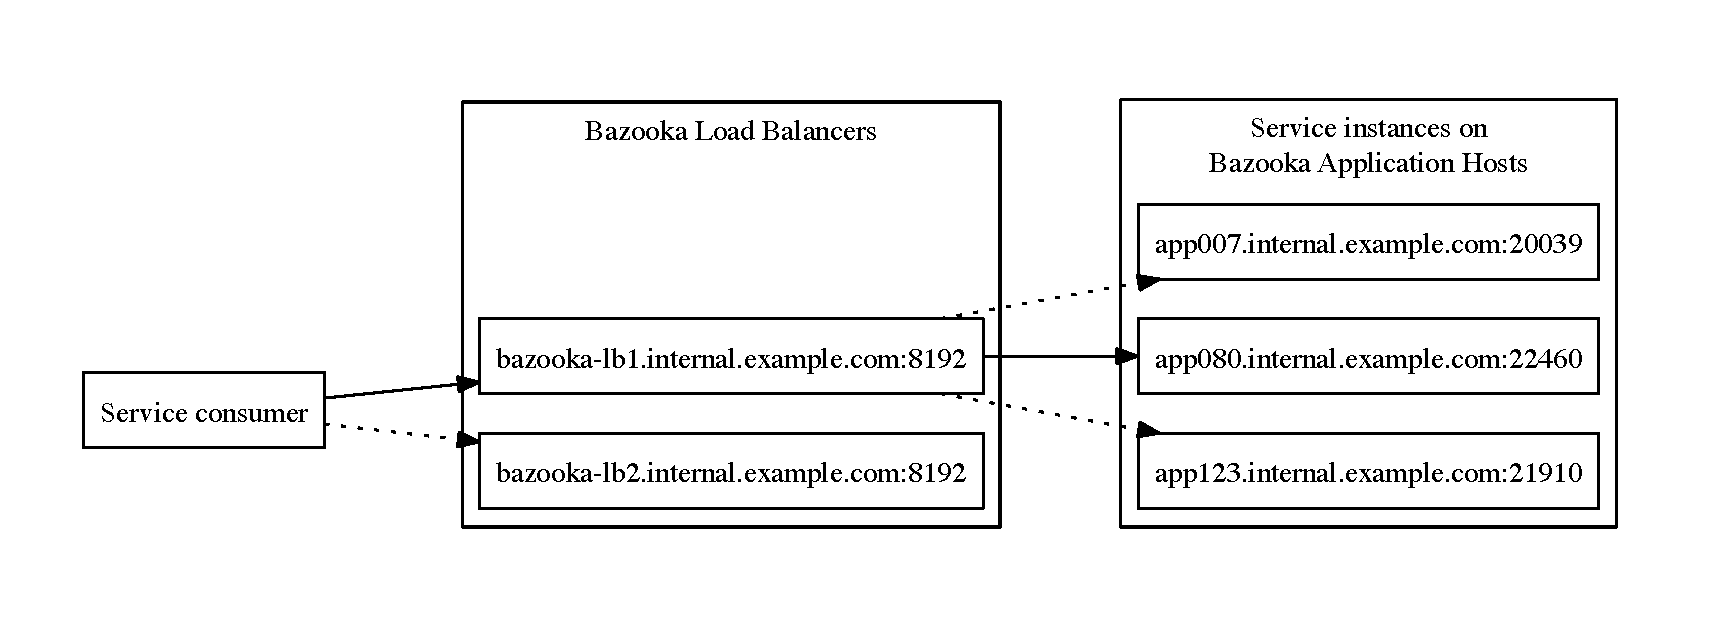
\includegraphics[width=\linewidth] {images/bazooka-lb-service-discovery.pdf}
  \caption{Visualization of the request flow from client to service through the Bazooka load balancer. Boxes represent machines with the domain name and port number as names. Solid edges represent the request flow. Dotted edges represent potential opportunities for different request flows, which would still yield the same results.}
  \label{fig:bazooka_lb_sd_example}
\end{figure}

\subsubsection{Glimpse}
\label{subsubsec:glimpse}

Glimpse is an application for service discovery, developed in-house of our case study. It is based on DNS SRV records (specified in RFC 6763~\cite{rfc6763}), which for one domain name allow to request many pairs of domain name and port number. The query domains have the following format:

\lstinline!{protocol}.{job}.{env}.{product}.{zone}.internal.example.com!
\begin{tdescription}
  \item[protocol] denotes the application-layer protocol with which to access the service. Examples are \emph{http} or \emph{ssh}.
  \item[job] is the name of the service in the context of the application. Examples are \emph{web} or \emph{admin}.
  \item[env] is the environment of the application deploy. Examples are \emph{production} or \emph{staging}.
  \item[product] denotes a grouping of user stories. It might match an application and repository name, but there is no convention enforcing that.
  \item[zone] denotes the zone, which a logical grouping of computing resources. Zones might for example be used to differentiate data centers.
\end{tdescription}

An example domain name is \\ \lstinline{http.app.prod.soundcloud.ca.srv.internal.example.com}

An example query is shown in \autoref{list:glimpsequeryexample}.

\begin{lstlisting}[caption=Service discovery via Glimpse; Query example ,label=list:glimpsequeryexample,numbers=none]
$ dig +short SRV http.app.prod.soundcloud.ca.srv.internal.example.com
0 0 5023 app117.internal.example.com
0 0 5023 app118.internal.example.com
0 0 5024 app097.internal.example.com
0 0 5024 app117.internal.example.com
\end{lstlisting}

The service discovery requests of Glimpse are handled via BIND~\cite{bind} DNS server. At the time of writing, two existed, which are the authoritative sources for the Glimpse DNS namespace. The namespaces are initially configured by engineers, but the actual service instance information for each glimpse domain is gathered and distributed to the DNS server automatically.

% Might also be used for bazooka deployed

% To summarize this section, table XXX shows for each method the mapping between one application name, respective intermediate formats and the eventual ipaddress:portname combinations.
%
% \begin{table}
%   \caption{Examples for the explained service discovery methods}
%   \label{tab:shortened_app_names}
%   \begin{tabular}{ |l|l|l| }
%     \hline
%     Service discovery key & Intermediate representation & Service location(s) \\
%     \hline
%     Physical Address (IP) \\
%     10.20.30.40 & & 10.20.30.40:2000 \\
%     \hline
%     Physical Addresses (Name) \\
%     app08.internal.example.com & 10.20.30.40 & 10.20.30.40:2000 \\
%     \hline
%     Semantic DNS CNAME \\
%     app.internal.example.com & app08.internal.example.com & 10.20.30.40:2000 \\
%     \hline
%     Bazooka \\
%     bazooka-lb.internal.example.com:3001 & 10.20.30.40:3001 (Bazooka load balancer) & 10.20.30.40:2000 \newline 10.20.30.41:2000 \\
%     \hline
%     Glimpse \\
%     http.web.prod.app.ca.srv.internal.example.com & & \\
%     \hline
%   \end{tabular}
% \end{table}

\subsection{Telemetry}
\label{subsec:telemetry}

Telemetry systems measure the state of a system, collect this information and make it available to engineers. During our investigations they were crucial tools for understanding and reasoning about the deployed architecture. Here we present three telemetry systems that were in use in our case study. More systems do exist, but we limit our descriptions to the ones that were relevant to our investigations.

\begin{tdescription}
  \item[Graphite]\cite{graphite} describes itself as doing two things: ``1. Store numeric time-series data 2. Render graphs of this data on demand''. Every time series consists of many datapoints. A series has a resolution, defining how many seconds of time each datapoint covers. In our case study, the standard resolution was 60 seconds. Data is sent to \emph{Graphite} via HTTP, setting the value for individual data points in time series. During querying, time series may be transformed and combined through functions. Graphite allows the extraction of the raw time series data as well as displaying visual graphs. In our case study, the majority of measures were collected and displayed with Graphite.
  \item[StatsD]\cite{statsd} describes itself as ``[a] network daemon that [...] listens for statistics, like counters and timers, [...] and sends aggregates to [...] backend services (e.g. Graphite)''. \emph{Graphite} only allows setting absolute numeric values for each datapoint. \emph{StatsD} allows for aggregating data for each datapoint before, for example when an event (like an HTTP request) happens, its result might be sent to \emph{StatsD}, which aggregates all of these events for the current datapoint and then sends that aggregated datapoint to \emph{Graphite}.
  \item[Prometheus]\cite{prometheus} describes itself as ``a generic time series collection and computation server''. Different to \emph{Graphite}, its data collection mechanism is pull-based: in regular intervals the \emph{Prometheus} server queries a telemetry HTTP resource on each measured instance. The instances internally aggregate the metrics.
\end{tdescription}

In our case study, \emph{Prometheus} is set to eventually replace the combination of \emph{Graphite} and \emph{StatsD}. At the time of our investigation, both systems were in use and served different measurements.

\section{Summary}

In this chapter we have introduced our case study, the berlin-based company ``SoundCloud'' in which the author was embedded while investigating this work. We have shown how the architectural style used in the case study has evolved from a monolithic multi-tier web application towards a microservice architecture (as visible in \autoref{fig:evolution_example}). We have also described concrete implementations of infrastructure systems, on which we will rely in the following chapters. As a problem in assessing the dependability of the deployed microservice architecture we identified a lack of visibility regarding the dependencies between applications.

  %!TEX root = ../master_thesis.tex

\chapter{Constructing dependency graphs}
\label{chapter:dependency_graph}

In this chapter we investigate how to construct a graph of application dependencies from a deployed and running microservice architecture. We first introduce the assumptions regarding the properties of the graph. Then we propose four methods for graph construction. We end the chapter by discussing and summarizing our findings.

\section{Theory}

In literature dependency graphs often are understood as ``program dependence graphs'' \cite{Horwitz} which model how a program works internally on the granularity of software modules, control flow or data flow. In this work, we use the granularity level of applications and dependencies between these as the basis for dependency graphs.

\subsubsection{Directed graph}

A \textbf{directed graph} (or ``digraph'') consists of \emph{vertices} and \emph{directed edges} \cite{ChartrandGary}. The edges connect the vertices. Every edge has a direction, leaving from one vertex and arriving at another vertex. All edges leaving from a vertex are called \emph{outgoing} edges. All edges arriving at a vertex are called \emph{incoming} edges.

\textbf{Vertices} represent applications in a microservice architecture.

Earlier in \nref{sec:software_environment_terminology} we established that one application has many processes and each process might implement or consume many services. Thus if there are many processes (or services) for one application in the graph, these would all be represented by one vertex for the application they belong to.

\textbf{Directed edges} represent service dependencies between applications.

A service dependency is the fact that a process is the consumer of a service (as explained earlier in section \ref{subsec:service_depenedency}). The direction of the directed edge follows the direction of the service dependency, from service consumer to service provider. If the vertices represent applications, the service dependency may exist for these as well, since processes and service always belong to exactly one application

\subsubsection{Example graph}

\nref{fig:digraph_example} shows a graphical example. It shows the following information:
\begin{titemize}
  \item Application A is dependent on Application B
  \item Application A is dependent on Application C
  \item Application B is dependent on Application D
\end{titemize}

\begin{figure}[h]
  \begin{center}
    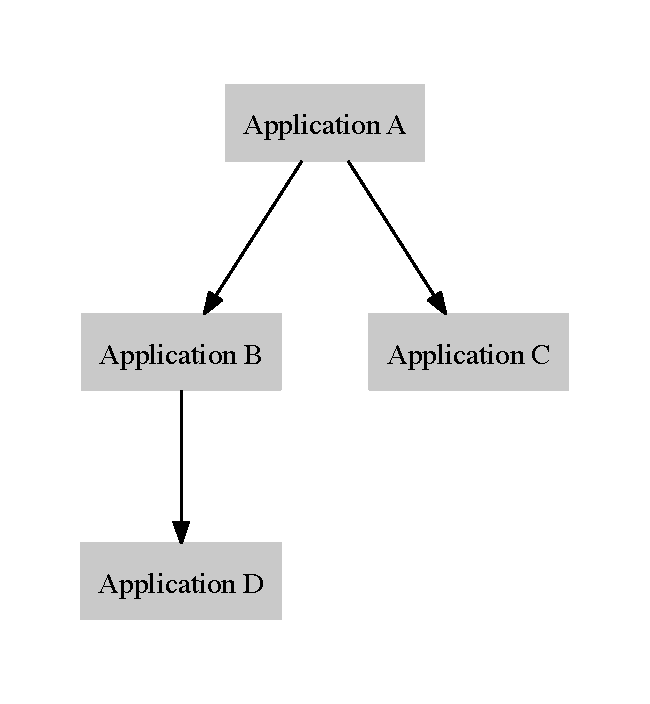
\includegraphics[width=0.48\textwidth]{images/directed-graph-example.pdf}
  \end{center}
  \caption{Dependency graph: example}
  \label{fig:digraph_example}
\end{figure}

\vfill\clearpage

\section{Methods for construction}

To construct a dependency graph from a deployed microservice architecture, we propose four methods in this chapter:
\begin{titemize}
  \item[] {\small\ref{subsec:graph_manual_annotation} \ncref{subsec:graph_manual_annotation}}
  \item[] {\small\ref{subsec:from_smi} \ncref{subsec:from_smi}}
  \item[] {\small\ref{subsec:graphfromdeploymentconf} \ncref{subsec:graphfromdeploymentconf}}
  \item[] {\small\ref{subsec:from_network} \ncref{subsec:from_network}}
\end{titemize}

We will discuss each of these methods after the following section structure: We first introduce the theory of the method based on our terminology model for microservice architectures from \nref{sec:software_environment_terminology}. The theory includes the assumptions the method makes against the environment it is executed in, and the high-level process of executing it. Afterwards we describe how we executed the method in the context of our case study and present the respective results. To conclude each section we discuss our findings. For that we evaluate each method after the following criteria:
\begin{tdescription}
  \item[Feasibility] Is it possible to execute the method at all?
  \item[Correctness] How well does this method detect all applications and dependencies?
  \item[Automation] To what extent can this method be automatically executed?
\end{tdescription}

\subsection{Manually creating a dependency graph}
\label{subsec:graph_manual_annotation}

This method is based on people manually creating the dependency graph.

The naive way of doing this is without a formalized process, but rather ad-hoc to the discretion of some people. This approach is limited by how much an individual person or a group of people may know about the whole architecture. With an increasing size of an architecture (quantified by number of applications and service dependencies) the generated graph will be more prone to include errors, since it will be less likely that the involved people have enough holistic knowledge about the architecture. In our case study we found several manually created diagrams representing application dependencies. They lacked a well-defined definition of the elements of the diagram and represented the architecture from a specific viewpoint only, but never showed a holistic view.

In this section we propose a semi-automated approach for generating a dependency graph for a deployed microservice architecture. It is based on people manually annotating the service dependencies of individual applications in a structured format. These annotations are then gathered in order to generate the dependency graph.

\subsubsection{Theory}

We base this approach on the following assumptions:

\begin{tenumerate}
  \item Every application has exactly one codebase
  \item Every codebase is tracked in a source code version control system
  \item Every codebase has one canonical repository location
  \item Every canonical repository location has a unique identifier within the scope of the microservice architecture
  \item It is possible to fetch a list of all repositories within the scope
\end{tenumerate}

Given these assumptions, we may do two steps: First we manually annotate each repository with its respective service dependencies. Then we gather all repositories and annotations to create the dependency graph.

We start by fetching a list of repositories. For each repository, we decide, if it constitutes an application that fits the criteria for being in the dependency graph. Example of applications that might be excluded are prototypes or historical codebases. If an application does not fit the criteria, it is not annotated. If it fits the criteria, an annotation for it is created. Each annotation holds a list of applications that the current application has service dependencies to. The application identifiers used are the repository identifiers.

Given that all annotations are created, we may create the directed graph from them. Each annotated application becomes a vertex in the graph. From the annotations of that application, each service dependency becomes an outgoing directed edge to the respective application providing that service.

Next, we will describe how we executed this method in our case study.

\subsubsection{In the case study}

All application repositories of our case study were kept under one GitHub organization. This provided a central unique naming scope for the repository identifiers. It also made it possible to fetch a list of all repositories. In our case study, we fetched 545 repositories.

We then decided for each repository, if it should be part of our investigation. We used the following criteria:
\begin{tenumerate}
  \item The application is currently deployed in the production environment
  \item The application is client-facing, thus it implements a functionality visible to users
\end{tenumerate}

This excluded many repositories, for example:
\begin{titemize}
  \item applications, which do not consume a service (like data storage system, which only provide a service)
  \item infrastructure applications, which do not directly satisfy user requests (like deployment and telemetry applications)
  \item deprecated applications, which are not deployed anymore
  \item prototype applications, which are not deployed in the production architecture
  \item shared libraries, which are not stand-alone applications themselves
  \item documentation, which are no applications at all
  \item one-off jobs, which do not directly satisfy user requests (like analytic aggregations)
\end{titemize}

We identified 75 applications fitting our criteria. For each of these, we manually created an annotation file in JSON\footnote{``JSON is a text format that facilitates structured data interchange between all programming languages''~\cite{json}} format. We defined our own annotation format, since existing dependency annotation systems like the dependency management tools \emph{Bundler}~\cite{Bundler} or the dependency management system of \emph{Go}~\cite{Go} (which we both describe in detail in the following \nref{subsec:from_smi}) were created with a focus on shared code library dependencies. Still we believe it would be possible to map our annotation format to other formats, given that these work with a ``manifest file'' like \emph{Bundler} does.

An example of an annotation file in our format can be seen in \autoref{list:manual_annotation}. It annotates the \emph{threaded-comments} application, which we will also work with in \nref{chapter:fault_trees}. As application identifiers we used URIs (as specified in \cite{rfc3986}). In the example, we see two kinds of application identifiers: The first one are URIs of web URIs of Github repositories. The second kind is a URI to the software project's homepage.

\pagebreak

\begin{lstlisting}[language=json,firstnumber=1,caption=Dependency graph: the manual annotation file in JSON format for the threaded-comments application ,label=list:manual_annotation]
{
  "dependencies": [
    "http://github.com/soundcloud/soundcloud",
    "http://github.com/soundcloud/authenticator",
    "http://www.memcached.org"
  ]
}
\end{lstlisting}

Given all annotation files, we created the dependency graph out of that. \autoref{fig:manual_annotation_whole} shows the graph for our case study. We created the graphical representation with Graphviz~\cite{graphviz}, which also orders the vertices hierarchically based on the edges. The hierarchical ordering has no semantic meaning applied by us. Furthermore we masked the application identifiers with numbers, in order to protect confidentiality of the case study company.

The following things can be seen in the visualized graph: In total, we identified 90 applications and 188 service dependencies. Towards the top of the graph are applications with no incoming edges. These applications are directly used by the clients. One can argue that the clients have service dependencies on these applications. We excluded clients from this investigation, thus these are not present. Several application show a high concentration of incoming edges: Vertex \emph{2} is the database application, vertex \emph{3} is the message queueing application and vertex \emph{5} is the former monolithic application.

\afterpage{%
\thispagestyle{empty}
  \begin{figure}[t]
    \vspace*{-3.5cm}
    \includegraphics[angle=90, width=0.85\linewidth]{images/arch-all-masked.pdf}
    \caption{Dependency graph: Manual annotation from case study with masked application names. Grey boxes are internal applications. Blue boxes with dotted outline are external applications.}
    \label{fig:manual_annotation_whole}
  \end{figure}
\clearpage
}

\subsubsection{Discussion}

In our case study we executed the application identification and dependency annotations by looking at the information in the repositories. This includes the source code, documentation, build information, required environment variables and packet management information. We also asked engineers and used information from the deployment system. Still, we assume that our method and our execution of it has a non-determined percentage of mistakes. We assume one way to reduce the percentage of mistakes is by deferring the responsibility to annotate the service dependencies to the teams that are responsible for the individual applications, since these are the individuals who probably know their applications best. We propose that the actual annotation file should then be kept within the application repository, e.g. as a file like ``service-dependencies.json''.

A problem with manual annotation is to keep the information up-to-date, e.g. when applications are retired or service dependencies change. This gap impedes on the correctness of the dependency graph and therefore raises the question of how much the generated graph may be trusted by engineers.

% If we assume that there is a constant percentage of erroneous information in a generated graph, than the absolute number of errors will grow with the size of the architecture. We may also assume

Given that several people annotate the dependencies, using unambiguous application identifiers becomes a problem. Getting unique identifiers is solved by using URIs that are reachable via the global DNS system. The more difficult requirement is if two people individually encounter an application, they need to assign the same identifier to it. This is easy for applications within the organization's scope, given that we assume unique repository identifiers, which can be used directly as application identifiers. But for external applications, we did not find an unambiguous convention, given that not all applications have a canonical repository location and not all applications have a canonical project website.

To conclude the discussion, we evaluate the method after the three criteria:
\begin{tdescription}
  \item[Feasibility] Given our experiences from executing the method in the context of the case study, we believe this method to be well feasible.
  \item[Correctness] The \textbf{correctness} of the generated graph directly depends on who creates it. If few people create it, the organizational overhead is low but the people involved may not have enough knowledge to create a holistic view of the architecture. If many people are involved in the creation, enough knowledge over the architecture may be contributed but the organizational overhead may be a significant burden. We believe that distributing the creation of the annotations to the teams building and maintaining the applications might be a way to provide an acceptable level of correctness, which should be investigated more in future work. The correctness of the method should also be seen over time: The dependency graph not only needs to be created once, but also maintained over time, given that architectures are very likely to change. We believe that the correctness of the generated graph eventually is a cultural problem of the engineering organization.
  \item[Automation] By the nature of the method, manual annotation is not \textbf{automated}. But given that distributed creation of annotation information might exist, the gathering of the annotations and subsequent generation of the dependency graph may happen automatically.
\end{tdescription}

\subsubsection{Future work}

We see manual annotations as a cultural problem. Future work might explore, how the creation and maintenance of manual annotations in an organization may be incentivized. This is especially a problem, since the benefits of annotations might not be immediately visible to their creators.

As another opportunity we see the possibility to combine manual annotations with the other methods introduced in this chapter. Other methods could provide indicators for applications and dependencies, but the eventual decision over an annotation would still be with a person.

\subsection{From service interface modules}
\label{subsec:from_smi}

In this section we propose another approach for generating a dependency graph. It is based on the assumption that all service dependencies of an application are encapsulated in service interface modules and thus extractable from the source code. Therefore this method would allow us to extract service dependencies exclusively from the source code by static code analysis.

\subsubsection{Theory}

To begin with, we assume that there is a list of applications and their respective codebases. An example for generating this list is through manual creation (as we also did in previous \nref{subsec:graph_manual_annotation}). Given that we have these applications, we may analyze their codebases.

The central assumption of this method is that access to service dependencies is encapsulated in ``service interface modules'' (short: SIM). A SIM is a software module within an application. It exists to encapsulate the access to specific service.

We see two kind of SIMs:
\begin{tenumerate}
  \item shared libraries, which usually encapsulate access to external services
  \item internal modules, which usually encapsulate access to internal services
\end{tenumerate}

Furthermore we make the following assumptions about SIMs:
\begin{titemize}
  \item From each applications's codebase it is possible to extract the used SIMs.
  \item It is possible to map a SIM to the application identifier it encapsulates.
\end{titemize}

Given these assumptions, for each application the SIMs may be extracted and matched to the accompanying applications. This results in a list of service dependencies per application. These may then be used to construct a dependency graph, by taking the applications as vertices and the service dependencies of each application as outgoing edges to the respective service-providing applications.

\subsubsection{In the case study}

To execute the approach in our case study, we start with a list of relevant application identifiers. We manually created this list after the same criteria as in previous \autoref{subsec:graph_manual_annotation}, which means we continue to work only with applications that are deployed in the production environment and serve a user-facing purpose. This list of application identifiers allows us to access the codebase for each application, since it coincides with the identifier for the repositories. Therefore, we may acquire the codebases for all applications and continue with the next step.

\begin{table}
  \caption{Approximate percentual statistics over languages of relevant applications in our case study.}
  \label{tab:SIM_language_stats}
  \begin{tabular}{ |l|l|l|l|l|l|l|l|l|l| }
    \hline
    Ruby & Go & Scala & Clojure & JavaScript & Python & Java & C++ & C \\
    \hline
    37\% & 16\% & 15\% & 8\% & 15\% & 2\% & 2\% & 4\% & 1\%\\
    \hline
  \end{tabular}
\end{table}

Given that the codebase is accessible, the process of extracting SIMs from it may be executed. In our case study, applications are written in a variety of programming languages~\cite{BourgonPolyglotGo}. Table \ref{tab:SIM_language_stats} shows a percentual breakdown of the application languages. We derived this information from the Github repository language determined via Linguist~\cite{linguist}. From the table it is visible that \emph{Ruby} and \emph{Go} are the most common programming languages, thus we started to investigate them first.

\subsubsection{Ruby}

% Next we investigate, how to extract ``service interface modules'' from Ruby~\cite{ruby} applications in our case study. We will first look at ``shared code libraries" and then at ``internal modules''.

In Ruby ``shared code libraries'' are packaged and distributed as ``Gems''~\cite{whatisagem}. In our case study we found all Ruby applications to use ``Bundler''~\cite{Bundler} to manage their Gems. Bundler is a dependency manager that facilitates loading the correct Gems as well as keeping these configurations portable when changing the execution environment. It does so by creating a manifest file (called ``Gemfile'') in the application's root directory. The Gemfile holds information about the needed Gems. Listing \ref{list:gemfile} shows a shortened Gemfile from an application of our case study. We did not find an automated way to determine the application identifiers for the encapsulated service dependencies from Gems. We believe this information to also be hard to generically exist, since the application identifiers might be dependent on the context of the individual organizational context. In our case study, we manually mapped Gem names to application identifiers by looking at the name of the Gems, the documentation for the Gems as well as our experience and asking engineers of our case study. Looking back at the example in \autoref{list:gemfile}, the 2 gems ``haml''~\cite{haml} and ``rack''~\cite{rack} do not encapsulate a service dependency, thus are no SIMs. The gem ``jberkel-mysql-ruby''~\cite{jberkel-mysql-ruby} encapsulate access to the \emph{MySQL}~\cite{mysql} application. The gem ``amqp''~\cite{amqp} encapsulates access to the \emph{RabbitMQ}~\cite{rabbitmq} application.

\begin{lstlisting}[caption=Shortened Gemfile from an application of the case study,label=list:gemfile]
[...]
source 'https://rubygems.org'

[...]
gem 'amqp',
[...]
gem 'haml',
gem 'jberkel-mysql-ruby',
[...]
gem 'rack'
[...]
\end{lstlisting}

For ``internal modules'', Ruby offers the constructs of classes, objects and modules to encapsulate software components. Due to its dynamic nature and facilities for sophisticated meta programming, we found it unreliable to extract these as SIMs from the source code. Furthermore, even if these could be reliably extracted, the mapping between SIM and encapsulated application would not be present.

\paragraph{Go}

% Next we investigate, how to extract ``service interface modules'' from Go~\cite{go} applications in our case study.

In Go the preferred way of separating software components is via packages. It is possible to extract a list of all imported packages from a Go application\footnote{In Go version 1.2, the following code returns a list of imported packages: \newline \emph{go list -f '{{join .Imports "\textbackslash n"}}'}}. Packages are identified during import via their path within the \$GOPATH directory. With this method, there is no distinction between ``shared code libraries'' and ``internal modules'', thus they may be treated the same.

As an example \autoref{list:go_imports} shows the shortened output of the list of imported packages for an application with identifier \emph{threaded-comments}. The packages \lstinline{flag} and \lstinline{fmt} belong to the standard library of Go. The package \lstinline{github.com/streadway/handy/breaker} is a shared library that does not encapsulate access to a service dependency. The package \lstinline{github.com/ianoshen/gomemcache/memcache} is a shared library that encapsulates access to the memcached~\cite{memcached} application. We were able to determine these mappings by manually looking at the packages' documentation. We did not find opportunities to automatically determine the mapping between package and application identifier. We were however able to identify, if a package opens a network connection\footnote{We did identify potential network connections by analyzing the abstract syntax tree of the codebase for calls to the ``net'' package's methods for opening network connections}. This might allow identifying candidates for SIMs, which then in turn could be mapped to application identifiers manually by a person.

% A common practice with Go is to copy shared library code into the codebase of the application (e.g. advised in \cite{goversion}).

\begin{lstlisting}[caption=Shortened list of imported packages of the thread-comments application,label=list:go_imports]
[...]
flag
fmt
github.com/ianoshen/gomemcache/memcache
github.com/streadway/handy/breaker
[...]
\end{lstlisting}

After the experience with these two languages, we did not investigate the extraction of SIMs for other languages. We expect them to work in similar ways with similar conclusions.

It is to note that in our case study, we did not find occurrences of access to internal services being encapsulated in shared libraries. Some service dependencies where encapsulated in internal modules though, but we did not find a way to map the respective application identifiers to them.

% isn't there a design pattern for encapsulating? proxy pattern?

Given these experiences, we did not generate a dependency graph via this method.

\subsubsection{Discussion}

Looking at the results from earlier \nref{subsec:graph_manual_annotation}, we see that the majority of service dependencies are between internal applications. In our case study execution we found that dependencies between internal applications are nearly never encapsulated in identifiable SIMs. Therefore, a dependency graph generated with this method would not include a large amount of existing service dependencies, impeding heavily on the completeness of this method.

When we identified SIMs in the case study execution, we were not able to match these to their respective application identifiers. The only option was to manually map them. Therefore, it does not seem possible to execute this method automatically.

One aspect that impedes on the feasibility of this method is the needed implementation effort. This method requires extensive knowledge about the used languages and their dependency management systems. Thus, there needs to be an individual implementation for each configuration, which in a polyglot environment constitutes significant effort.

% Some SIMs (like carrierwave, amqp) encapsulate access to several applications.

To conclude the discussion, we believe that this method is not well \textbf{feasible}. Given the problems with identifying internal applications, we believe the resulting dependency graphs to significantly lack \textbf{completeness}. This method may be executed \textbf{automatically}, given the problem of mapping SIMs to application identifiers is solved in an automated way.

Future work might investigate the creation of a database of SIM-to-application-identifier mappings. When a person manually annotates a  ``shared code libraries'' or ``internal modules'', this mapping could be then used in subsequent executions of the method, which would reduce the total amount of manual mapping work needed in many executions of the method.

% As a second option for future work, the extracted ``shared code libraries'' or ``internal modules'' could be used as candidates for service dependencies.

\subsection{From deployment configuration}
\label{subsec:graphfromdeploymentconf}

With the method we introduce in this section, a dependency graph may be generated based on the service dependencies extracted from application deploys. To do so, the values of the deploy's configuration are examined and mapped to application identifiers via reverse service discovery.

\subsubsection{Theory}

We base this method on the following assumptions:

\begin{tdescription}
  \item[Applications are configurable] Applications are built in a way, such that external configuration, which tailors the application to the current execution environment, might be injected when the application is started. Examples of configuration are enabling or disabling features (e.g. logging, debugging, choosing algorithms) and setting thresholds (e.g. timeouts, queue sizes).
  \item[Applications are configured during deployment] We assume that all applications are deployed with the help of a deployment system (like outlined for our case study in earlier \nref{subsec:deploymentsys}). The deployment system compiles the configuration for the deploy and makes it available to the processes. The format of the configuration is not relevant here; examples are operating system environment variables or configuration files. The exact configuration details may be gathered from different sources, like a database or the runtime information from the currently deployed architecture.
  \item[Service discovery is part of the configuration] Service discovery is the process of finding the service instances of a certain application deploy (as explained earlier in \nref{subsec:servicediscovery}). We assume that service discovery happens to a certain extent during the deployment process and is present in the configuration, thus allowing the execution of \emph{reverse service discovery} on the configuration values. We use the term reverse service discovery to describe the process of mapping a service discovery key, service location, intermediate value of the service discovery process to its respective application identifier.
\end{tdescription}

Given these assumptions, we may execute the method as follows:
\begin{tenumerate}
  \item Fetch a list of relevant application deploys.
  \item For each deploy, we need to have access to the currently deployed configuration.
  \item For each configuration, we go through all values and identify the ones that are service locations. For each service location we then identify the respective application identifier via a reverse service discovery lookup.
\end{tenumerate}

\vfill\clearpage

Resulting from this method is a list of deploys and therefore also applications\footnote{We assume that for every deploy identifier, the corresponding application identifier is derivable. A simplest case is, if the deploy identifier is the same as the application identifier. Another case is, if the application identifier is part of the deploy identifier and can be parse out of that (e.g. \lstinline{deploy identifier: "app-env" => application identifier: "app"}).}. For each deploy, a list of service-providing applications exists. We may then generate a dependency graph out of that information: Every deploy is a vertex. Every service dependency becomes an outgoing edge from the deploy to the service-providing application.

\subsubsection{In the case study}

Next we describe how we executed the method in the context of the deployment system Bazooka. For the other deployment systems (explained in \nref{subsec:deploymentsys}) we were not able to reliably identify deploys and their respective environments, thus we did not execute the method with them.

In Bazooka we may fetch a list of all application deploys from Bazooka's distributed data store. In our case study this list also included staging and prototype deploys, which we manually removed from the list since we were only interested in deploys in the production environment. Given this list we fetched the current configuration for each deploy~\footnote{In Bazooka, an application might have processes deployed with different environments. A typical case is a canary process~\cite{canary}. When we encountered such a case, we chose the most recent environment.}. In Bazooka the configuration is a list of key-value pairs. We extracted all values and used the methods explained next to map these to application identifiers. Listing \ref{list:bazookaconfexample} shows an example of such a configuration.

Through reverse service discovery, the values from the configuration may be mapped to application identifiers. Next we will introduce several methods for doing so. These relate strongly to the service discovery mechanisms we described earlier in \nref{subsec:servicediscovery}.

\pagebreak

\begin{lstlisting}[caption=Example configuration of an application in Bazooka,label=list:bazookaconfexample]
{
  "logLevel": "error",
  "threadedCommentsHost": "bazooka-lb.internal.example.com:8485",
  "soundcloudAppURI": "http.app.prod.soundcloud.ca.srv.internal.example.com",
  "databaseTransactionalAddress": "10.20.30.10:1337",
  "databaseAnalyticalAddress": "db04.internal.example.com:1233"
}
\end{lstlisting}

\textbf{Bazooka} To consume services deployed with Bazooka, consumers may use the Bazooka load balancer. For a service consumer to use a service, it has to know the port on the Bazooka load balancer. Therefore, in the configuration of a deploy, the Bazooka load balancer address and port number may be used (as visible in \ref{list:bazookaconfexample} for the ``threadedCommentsHost''). For our purpose of generating a dependency graph, we may map this port number to the application identifier, as described next:

Bazooka is using HAProxy as load balancing software. It is configured via a configuration file~\cite{haproxyconf} generated by Bazooka.  We may use that configuration file for doing reverse service discovery, from the Bazooka port number to the application name. Listing \ref{list:haproxyconfthreaded} shows a part of the Bazooka HAProxy configuration file for the threaded-comments application. The relevant part is the first line, which shows the port number (\emph{8485}) on the bazooka load balancer as well as the application-process-type combination (\emph{threaded-comments-web}) which, if split on the last hyphen, reveals the application's identifier. Since the port number is used by the clients, we assume it to not change during the further development of Bazooka. On the other hand, splitting the application-process-type combination is only possible as long this string stays the same. Since it is an internal implementation detail of Bazooka, this might change in future versions of Bazooka.

\begin{lstlisting}[caption=Bazooka HAProxy configuration file excerpt for the threaded-comments application,label=list:haproxyconfthreaded]
listen threaded-comments-web bazooka-lb.internal.example.com:8485
  bind-process 1
  server threaded-comments-web0 app08.internal.example.com:1000 [...]
  server threaded-comments-web1 app09.internal.example.com:3001 [...]
  [...]
\end{lstlisting}

\textbf{Glimpse} With Glimpse, a service is identified via a URI following a well-defined format. In previous listing \ref{list:bazookaconfexample}, the key ``soundcloudAppURI'' has such a URI as value. Given that the format is well-defined, it is possible to extract the \emph{product} information from it\footnote{Glimpse URIs are specifically meant to be parseable by regular expressions.}. The \emph{product} information may then be used as application identifier.

\textbf{Semantic DNS CNAMEs} A service might be identified via a URI with a DNS CNAME on an internal DNS namespace. In our case study, these followed a format similar to
\emph{{name}.internal.example.com}. The \emph{CNAMEs} were assigned manually by engineers. Given that these URIs follow a well-defined format, it was possible to identify URIs following it and extract the names from there. There is no convention around the usage of these names, therefore the name might or might not be an application identifier.

\textbf{Physical Addresses} In previous listing \ref{list:bazookaconfexample}, the keys ``databaseAnalyticalAddress'' and ``databaseTransactionalAddress'' use physical addresses for denoting service locations. Our only way to map these to application identifiers is by manual intervention. This might involve semantically interpreting the URIs or key name, or connecting to the denoted machine to investigate running processes.

With these methods for reverse service discovery to our disposal, we investigated them in the context of our case study. We executed this investigation on May 30th. We fetched all current deploys from Bazooka (296 deploy identifiers) that had running processes (reduced to 136 deploy identifiers). We manually removed deploys that were not part of the production architecture, like staging and prototype deploys as well as internal productivity applications. This reduced the number of relevant deploy identifiers to 90. For each of the remaining deploys, we fetched the latest configuration.

For each deploy configuration value we executed the just-introduced automatic reverse service discovery methods. For method \emph{Bazooka}, we had a list of addresses for the Bazooka load balancers. For method \emph{Glimpse}, we used the \emph{product} value as application identifiers. For method \emph{Semantic DNS CNAMEs} we used the extracted names as application identifiers.

Subsequently we were able to generate the dependency graph: Each deploy's application identifier became a vertex in the graph. Each of the discovered dependencies became an outgoing vertex from the deploy's application identifier to the identified service-providing application. The resulting graph can be seen in \autoref{fig:deploy_env_auto}.

\afterpage{%
\thispagestyle{empty}
  \begin{figure}[t]
    \vspace*{-3.5cm}
    \centering
    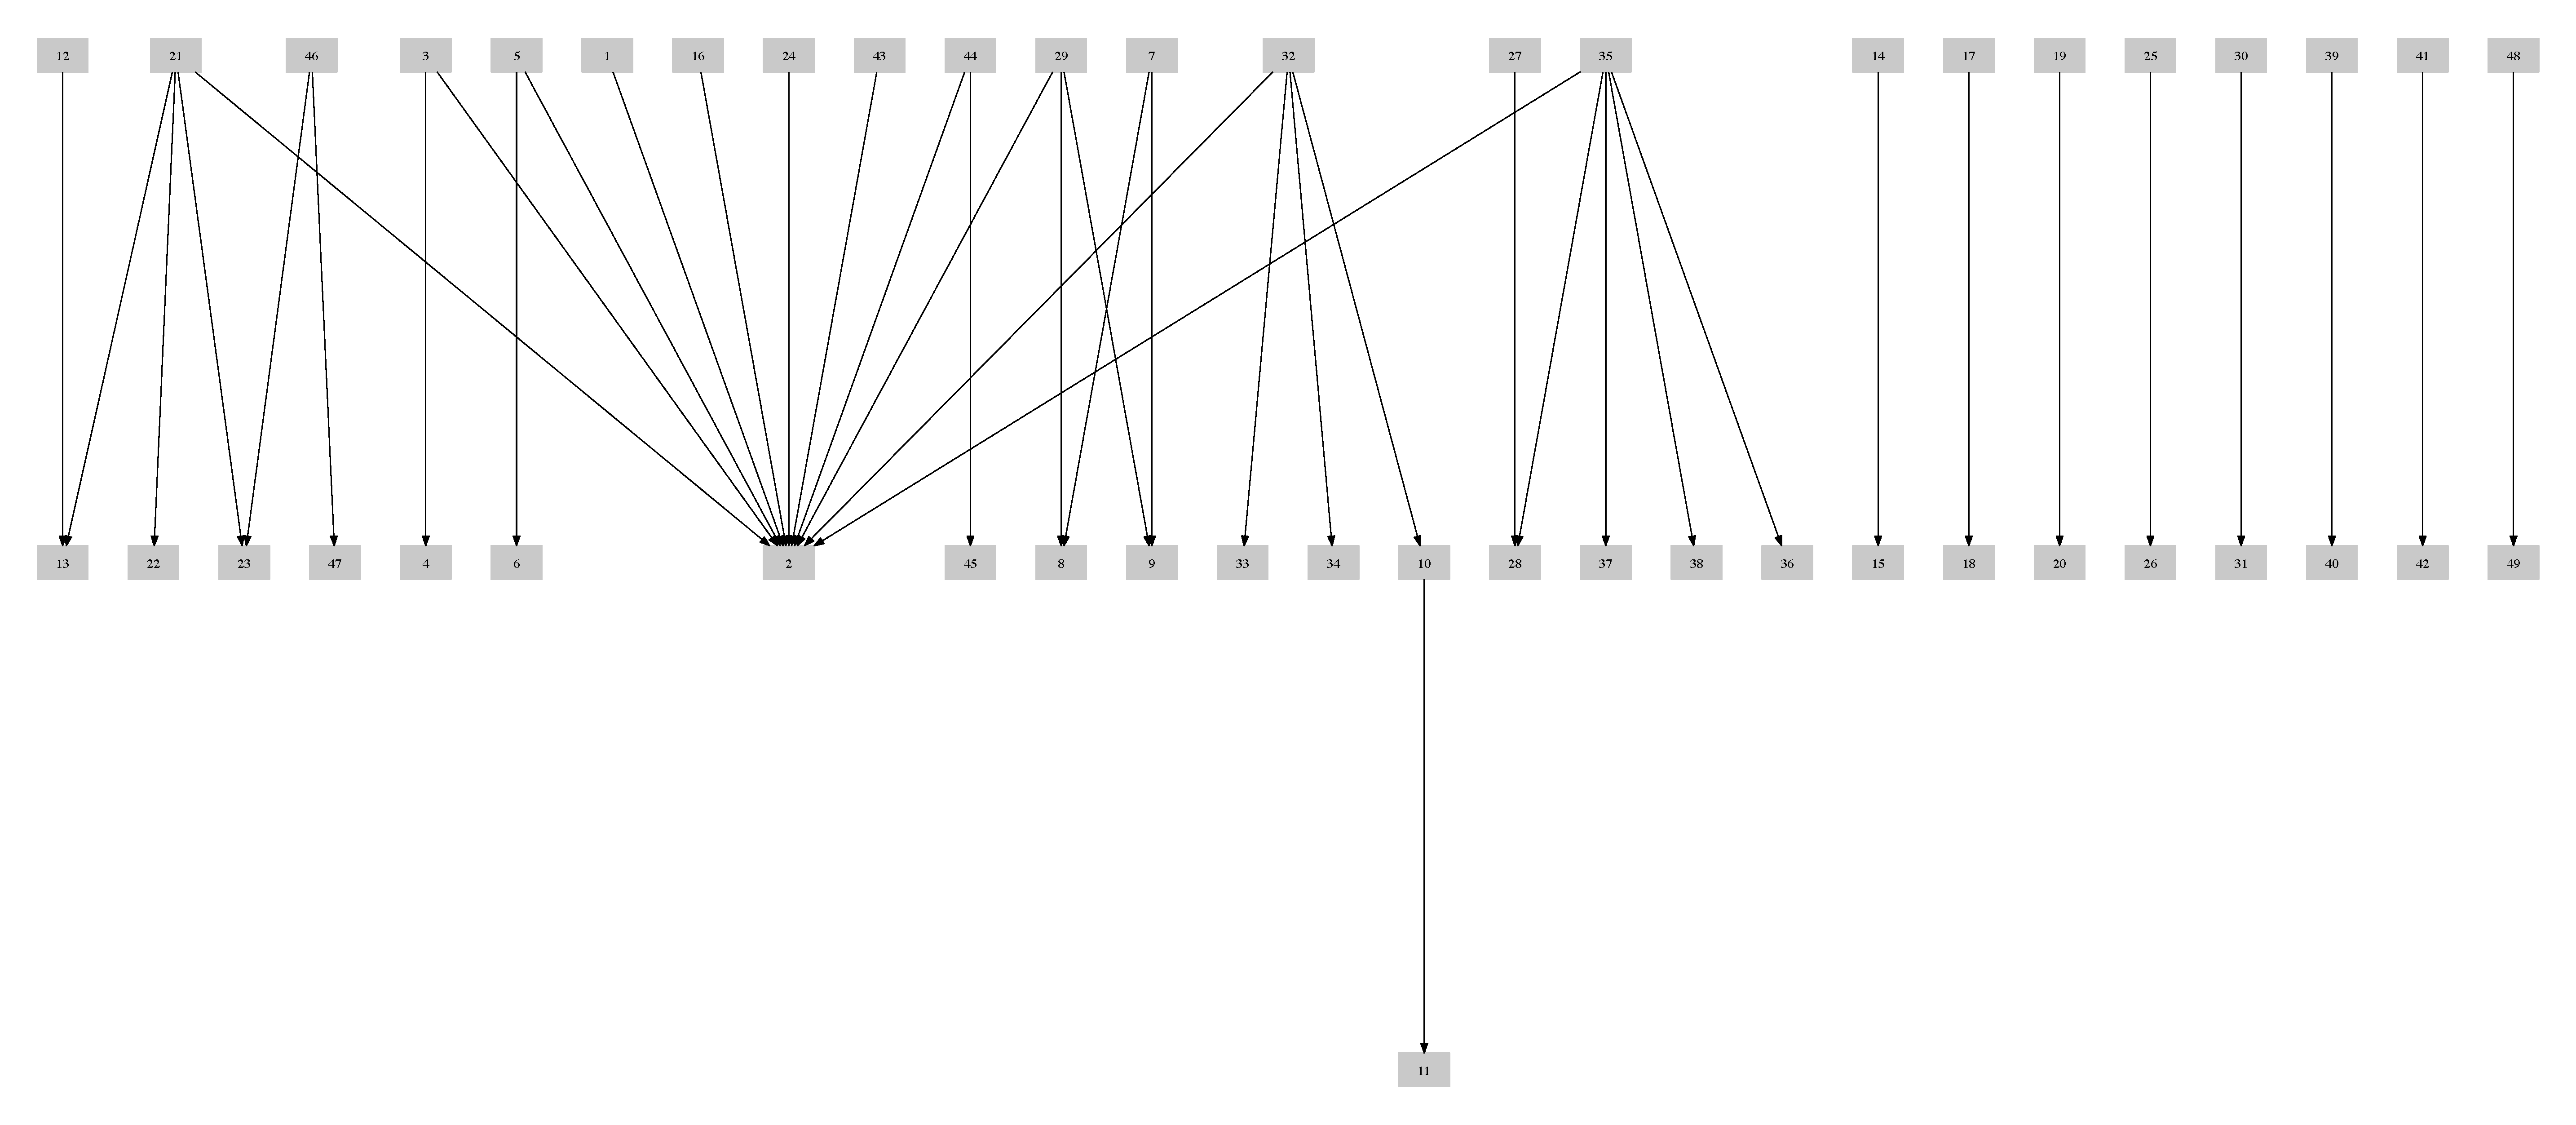
\includegraphics[angle=90, width=0.70\linewidth]{images/bazooka-masked-new-fixtures-bazooka-auto.pdf}
    \caption{Dependency graph generated from deployment configuration and executed with \textbf{automatic reverse service discovery} in the case study. The application identifiers are masked with incremented numbers.}
    \label{fig:deploy_env_auto}
  \end{figure}
\clearpage
}

To cross-validate these results, we manually determined the application identifiers for each value, taking the value and key name into account. The resulting graph can be seen in \autoref{fig:deploy_env_manual}.

\afterpage{%
\thispagestyle{empty}
  \begin{figure}[t]
    \vspace*{-3.5cm}
    \centering
    
\includegraphics[angle=90, width=0.50\linewidth]{images/bazooka-masked-new-fixtures-bazooka.pdf}
    \caption{Dependency graph generated from deployment configuration and executed with \textbf{manual reverse service discovery} in the case study. The application identifiers are masked with incremented numbers.}
    \label{fig:deploy_env_manual}
  \end{figure}
\clearpage
}

\subsubsection{Discussion}

We start the discussion by comparing the manually and automatically generated graphs with each other. The major difference between both are the sizes of the graphs. The automatically generated graph \ref{fig:deploy_env_auto} has 49 vertices and 41 edges, whereas the manual graph \ref{fig:deploy_env_manual} is about double as big with 88 vertices and 99 edges\footnote{Please note that between the different graphs, the numbering of the applications is not consistent. Thus, application ``1'' in one graph is not the same as application ``1'' in another graph. This is due to the mechanism of masking we used, which did not sync naming between the generation of the graphs.}. We attribute this difference to the fact that in the manual execution we have all reverse service discovery methods of the automated version available, plus are able to deal with edge cases manually. These included the following:
\begin{tdescription}
  \item[Decomposed URIs] We found 5 URIs that were decomposed into several configuration variables. One example for that is splitting the hostname and the portname into two variables, as visible in \autoref{list:bazookaconfexamplesplit}.
  \item[Incomplete URIs] 7 times we encountered URIs that did not fully denote a service. One example is the bazooka load balancer address as configuration value without the port number, as visible in \autoref{list:bazookaconfexamplesplit}, when only taking the ``bazookaLB'' variable into consideration.
  \item[Physical addressing not resolvable] We encountered several physical addresses, which were not automatically resolvable. We were able to resolve these manually with the help of the variable name as well as by logging into the respective machine and investigating the applied chef roles.
\end{tdescription}

Both graphs show the monolith of the architecture with a big number of incoming edges (vertex ``2'' with 11 incoming edges in the automated and vertex ``5'' with 13 incoming edges in the manual graph). We have seen the monolith to be mostly addressed via \emph{CNAMEs} with the application name. The database \emph{MySQL} (vertex ``2'') makes up for a significant share of the edges in the manually-created graph \autoref{fig:deploy_env_manual}. These are not represented in the automatically-addressed graph, since they addressed specific deploys of the application by IP address or physical machine name.

\begin{lstlisting}[caption=Example configuration of an application in Bazooka,label=list:bazookaconfexamplesplit]
{
  "bazookaLB": "bazooka-lb.internal.example.com",
  "threadedCommentsBazookaPort": 8485
}
\end{lstlisting}

% As long as there is no convention around how environment variables are structured, it will be hard to run this satisfyingly. Since the definition of these edge cases is subject to the creativity of the developers, we believe it will be impossible to handle all these edge cases completely.

\begin{table}
  \caption{Distribution of configuration cases for the dependency graph generated with manual reverse service discovery in \autoref{fig:deploy_env_manual}.}
  \label{tab:env_var_percentages}
  \begin{tabular}{ |l|l| }
    \hline
    Metric name & Value \\
    \hline
    Total number of configurations & 90 \\
    \hline
    Configurations without any variables & 17 \\
    Configurations with at least one variable & 73 \\
    \hline
    Configurations without any reverse service discoverable variables & 39 \\
    Configurations with at least one reverse service discoverable variable & 51 \\
    \hline
    Total number of dependencies discovered & 99 \\
    \hline
    Dependencies reverse service discoverable via Bazooka & 7 \\
    Dependencies reverse service discoverable via Glimpse & 1 \\
    Dependencies reverse service discoverable via CNAME & 65 \\
    Edge cases only service discoverable manually & 26 \\
    \hline
    CNAME discovered services directly mapping to an application name & 39 \\
    CNAME discovered services being deploys of the MySQL application & 22 \\
    CNAME discovered services being deploys of the RabbitMQ application & 4 \\
    \hline
  \end{tabular}
\end{table}

Table \ref{tab:env_var_percentages} shows more information about the distribution of the configuration. It can be seen that CNAME reverse service discovery makes up the majority of the discovered services. One of the assumption around CNAME discovery was that the \emph{name} is an application identifier. We found this assumption fulfilled in 60\% of cases, with the other cases denoting specific deploys of the \emph{MySQL} or \emph{RabbitMQ} applications (e.g. \lstinline{broker001.m.internal.example.com}).

In our investigations, we only found 1 case using the Glimpse service discovery. In that case, the ``product'' part of the URI did map the application identifier. Still, our method would benefit from either the convention that the ``product'' has to map the application identifier, or from another URI part that would include the application identifier. Among all methods of reverse service discovery, Glimpse proved to be the easiest to use. This is due to its well-defined URI format, which can be easily identifier via a regular expression, as well as the possibility to extract the identifiers without querying another system.

When comparing the graphs of this method with the earlier graph \nref{subsec:graph_manual_annotation}, we can see that the earlier graph has more vertices and edges (90 vertices/188 edges) than our graphs here (manual 88 vertices/99 edges and automated 49 vertices/41 edges). The earlier graph also has 7 hierarchy levels, whereas the graphs of this method only have 4 hierarchy levels. We attribute this to the fact that the graphs generated with the method here may only take applications into consideration which have been deployed with Bazooka, whereas the earlier graph may also take differently-deployed applications into consideration. It is to be noted that the comparability of the graphs is limited by the fact that there were several months between the generation of these graphs and more applications were created within this time period which are not present in earlier graph \nref{subsec:graph_manual_annotation}.

% Packet forwarding and domain aliasing make reverse service discovery more  complex. In our case study, one of these examples is the HAProxy load balancer by Bazooka, which

% precision/recall?
% Might have false-positives (if configuration has more, e.g. because legacy)
% Might have false-negatives (if not all service discovery is in configuration, which might happen)

One limitation during our investigation was the reverse service discovery for applications outside of the organizations scope like third-party services. Two practical examples we encountered in our investigation were the REST API of Twitter~\cite{twitterdev} as well as the Amazon S3 web services APIs~\cite{amazons3}. It would theoretically be possible to put these behind the internal service discovery mechanisms, but doing so is impractical, since it increases complexity without providing tangible direct benefits especially since the location of these external services is highly unlikely to change. Therefore we believe, these have to manually be mapped to application identifiers then.

To conclude, we have seen that the approach introduced in this chapter is \textbf{feasible}, since we were able to execute it in our case study. Its \textbf{correctness} and the degree of \textbf{automation} are influenced by how many of the requirements are met: Are all applications configured during deployment? Do all applications get their service dependency locations from that environment? Is it possible to obtain the configuration for the deploys? Is it possible to execute reverse service discovery for discovered service discovery locations? To structurally fulfill these requirements, we see deployment systems like Bazooka and service discovery systems like Glimpse as enabling factors.

\subsubsection{Future Work}

During the automated execution, we did not take the variable names into consideration. We did so during manual execution though. We found that variable names did not follow a convention. Still, they were useful in manually determining the service dependency application, even though this eventually meant ``guessing'' the actual application identifier. This could be improved by introducing a convention on environment variable names, which includes the application identifier. An example format is ``service\_{application\_identifier}''.

If the service locations are within the application's codebases and not in the environment, it might still be possible to execute this method. This assumes that we can extract the service locations from the codebase. We may then execute the same reverse service discovery mechanisms as explained before.

% Another method to handle service discovery is to do it within the application. An example is Zookeeper~\cite{zookeeper}, which is a distributed data store that was used as the basis for several service discovery systems in microservice architectures . Simplified, service discovery happens by accessing data in the zookeeper data store. Given we would be able. Instead of getting application dependencies from the environment, these might also exist within the application, for example if service discovery happens with Zookeeper. Then, would need to parse out of code all callsites for zookeeper and search for the key it is called with.

One of the edge cases we identified was physical addresses (e.g. IP addresses like  \emph{10.23.0.10} or physical domain names like \emph{app08.internal.example.com}). These do not hold service discovery information. If it is possible to connect to that address (e.g. via \emph{ssh}), investigations on the server could happen. Examples are investigating running processes (assuming a way to map processes to application identifiers) or applied chef roles (assuming a mapping from chef role to application). Both examples assume that a machine only has one application running.

\subsection{From network connections}
\label{subsec:from_network}

With this method we generate a dependency graph from the service dependencies of applications. We derive these service dependencies by observing network traffic and matching the source and destination processes to applications.

\subsubsection{Theory}

We assume that all application dependencies manifest themselves as network communication between the applications' processes. Thus if we detect network communication between two processes, we can derive that there is an application dependency between these applications.

To execute this method, we have to observe network communication. Assuming that communication is based on TCP/IP~\cite{internetprotocol}, we may take a TCP packet as atomic entity. A packet holds the information about the IP address and port number of the source and destination. If these can be mapped to their respective applications, we have determined the application dependency. If we are able to determine, which of the two communication parties started the communication, we can derive the direction of the application dependency, from source to destination.

Given all this information, the longer we observe the system, the more service dependencies may be collected. Each source or destination application becomes a vertex in the dependency graph and each observed service dependency becomes an edge.

\subsubsection{In the case study}

In our case study we executed this method in the context of applications deployed with Bazooka. We observed packets on the Bazooka application hosts. Each application host used a Linux distribution as operating system. We execute the packet observation using \emph{netstat}, which allows to display currently active network connections.

\begin{lstlisting}[caption=Sanitized example output from netstat. Schema is: local\_address foreign\_address process\_id/process\_name,label=list:netstatexample]
192.168.100.1:39998 192.168.100.3:1001 10411/application
192.168.100.1:2001 192.168.100.2:35019 20471/python
\end{lstlisting}

Listing \ref{list:netstatexample} shows an example output from netstat, which we filtered to include only the essential information. The IP address \emph{192.168.100.1} belongs to the machine where the capturing happened. The first line shows a connection that started from a local process to a remote service (\emph{outgoing connection}). The second line shows a connection that started from a remote process to a local service (\emph{incoming connection}). Next we will investigate for both cases, how to map the source and destination applications of the connection.

% A connection may either originate remotely (from another process to the machine currently under investigation) or locally (from the machine currently under investigation).

\paragraph{Source application} When a process opens a new network connection, it usually does so by using network sockets~\cite{sockets} \cite{SocketsProgramming}. A socket needs a local port, which it usually gets assigned by the operating system~\footnote{It is also possible for a process to bind to a specific local port. From our experience, this is common for server processes, since the location of their service has to be known to its clients. It is uncommon for client processes, since any port number works equally well, and a client process binding to a specific port number might get the problem of the port number already being occupied. Letting the operating system handle the concern alleviates the client process from the complexity of finding a free port number.}. If we now observe an incoming connection on a machine, there is no way to map that incoming port number to a process and/or application, since the port number has been assigned just for that connection.

Therefore we may only be able to map outgoing connections to application identifiers. Next we will describe that process in the context of the Bazooka application host. In the outgoing connection in \autoref{list:netstatexample} (first line) we can see that netstat returns a \emph{process\_id} and the \emph{process\_name}. The \emph{process\_name} does not reveal the application name, since processes have widely differing ways of being executed, resulting in no consistent mapping to application names. To do the mapping in our case study, we relied on implementation details of Bazooka: When a process is started on a Bazooka app host, it is executed within a Linux container (LXC~\cite{lxc}~\cite{lxcsuse}). These containers are isolated using Kernel Control Groups (cgroups~\cite{cgroups}). Via the proc virtual filesystem, it is possible to access the cgroup information for a specific process, which in turn contain the name of the container. Listing \ref{list:cgroupsexample} shows an example output of the cgroup information. Bazooka uses the following scheme for the container names: \newline \lstinline!{application}-{process}-{git-commit-sha}!. \newline We are able to extract the application identifier from that container name, and thus are able to map the source application for outgoing connections.

\begin{lstlisting}[caption=Cgroup information example from the proc virtual filesystem\, retrieved via \lstinline{cat /proc/20471/cgroup} in our case study,label=list:cgroupsexample]
1:perf\_event,net\_cls,freezer,devices,memory,cpuacct,cpu,cpuset:
  /lxc/threaded-comments-web-b3d7941-22160
\end{lstlisting}

\paragraph{Destination application} We have just shown that it is possible to obtain the source application identifier for \emph{outgoing connections}. Now we will show how to obtain the destination application identifier for such connections. The destination of a connection (or \emph{service location}) has the property that is has to be discoverable for the process wanting to connect to it. Commonly this discovery from a service discovery key to a service location is done via a service discovery mechanism. We are interested in doing this process in reverse, thus mapping from service location to the service discovery key and the to the application identifier. We call this process ``reverse service discovery'' and introduced several methods for it in the previous \nref{subsec:graphfromdeploymentconf}. The difference to the earlier execution and here is that we now only have IP addresses to work with. For example in the earlier listing \autoref{list:netstatexample}, the destination application has the IP address/port number pair of \lstinline{192.168.100.3:1001}. Next we will explain the execution for the Bazooka and Glimpse reverse service discovery:

\textbf{Bazooka} A service that is deployed with Bazooka is accessed via a port on the Bazooka load balancers. Given that we know the IP addresses of the Bazooka load balancer and have access to the HAProxy config file, we may map the application identifier the same way as introduced in earlier in \nref{subsec:graphfromdeploymentconf}.

\textbf{Glimpse} When we introduced reverse service discovery for Glimpse in earlier \nref{subsec:graphfromdeploymentconf}, we saw that the domain name format makes it possible to directly parse out the \emph{product} and therefore application identifier from a Glimpse service discovery domain.

To do the same in this method, we have to first map the IP address and port name to the Glimpse domain name. The Glimpse service discovery mechanism is based on BIND~\cite{bind}, which holds the information about the DNS mapping in a zonefile. Listing \ref{list:depgraphglimpse} shows an example excerpt from that zonefile. We can see that the product \emph{threaded-comments} has three instances. Each of these is identified with a physical domain name (e.g. \emph{app08.internal.example.com}) and a port number (e.g. \emph{1001}). Let's assume that we try to resolve the IP address \lstinline{192.168.100.3:1001} from earlier netstat example \autoref{list:netstatexample}. We first have to map the IP address to a physical domain name. We may do so with a reverse DNS lookup from address to domain name (as specified in RFC \cite{rfc1034} section 5.2.1.). Our example IP address \lstinline{192.168.100.3:1001} would then map to the physical domain name \emph{app08.internal.example.com}. We may use that physical domain name and the port number for a lookup in the zonefile, which leads to the Glimpse domain \emph{http.web.prod.threaded-comments.ca} and the product/application identifier \emph{threaded-comments}\footnote{It might be possible, to do reverse DNS lookup for SRV records, similar to reverse DNS lookups for IP addresses to domain names. Following the definition in RFC 6763 \cite{rfc6763} and our experience, we did not find a solution for that, other than the one introduced using the zonefile directly.}.

\begin{adjustwidth}{-0.9in}{-.8in}
    \begin{lstlisting}[caption=Glimpse zonefile example excerpt,label=list:depgraphglimpse]
      http.web.prod.threaded-comments.ca 5 IN SRV 0 0 1000 app08.internal.example.com
      http.web.prod.threaded-comments.ca 5 IN SRV 0 0 1001 app08.internal.example.com
      http.web.prod.threaded-comments.ca 5 IN SRV 0 0 5671 app78.internal.example.com
    \end{lstlisting}
\end{adjustwidth}

% \textbf{Semantic DNS CNAMEs} As already discussed in \nref{subsec:graphfromdeploymentconf}, engineers may assign CNAME domains to certain machines. These names may then be used as application identifiers during reverse service discovery. To discover the semantic CNAME for an IP address, we may use a reverse DNS lookup (as specified in RFC \cite{rfc1034} section 5.2.1.).

In our case study we executed the connection gathering and analysis with both reverse service discovery methods on March 14 2014. Next we will describe the process we used:
\begin{titemize}
  \item We executed the connection observations sequentially on all Bazooka application server. On each server, we executed netstat 50 successive times with a 5ms delay between the executions. We then collected the cgroup records for all processes on each application host\footnote{ This is based on the assumption that processes do exist for an extended amount of time, but at least between doing the connection observation and retrieving the mapping between process ID and cgroup. We found that to be true, with process IDs only changing when a process was restarted (for example when it crashed or a new deployment was done) or when it was stopped for administrative reasons (for example when the number of running process instances per deploy is decreased)}.
  \item We collected the zonefile from a BIND server by Glimpse\footnote{All instances of BIND in Glimpse used the same zonefile.}.
  \item We collected the HAProxy configuration file from a Bazooka load balancer\footnote{All instances of the Bazooka load balancers used the same HAProxy configuration file.}.
  \item We manually determined the addresses of all Bazooka load balancers.
  \item To analyze the data, we took each collected network connection and tried to map that to an application dependency with the methods explained above.
\end{titemize}

As a result of the investigation, we were able to derive 260 connection pairs between processes running on a Bazooka app host and a remote host. Of these, we resolved 9 application dependencies via the Bazooka load balancers and 2 application dependencies via Glimpse. Figure \ref{fig:graph_from_network} shows the resulting graph.

\begin{figure}[h]
  \begin{center}
    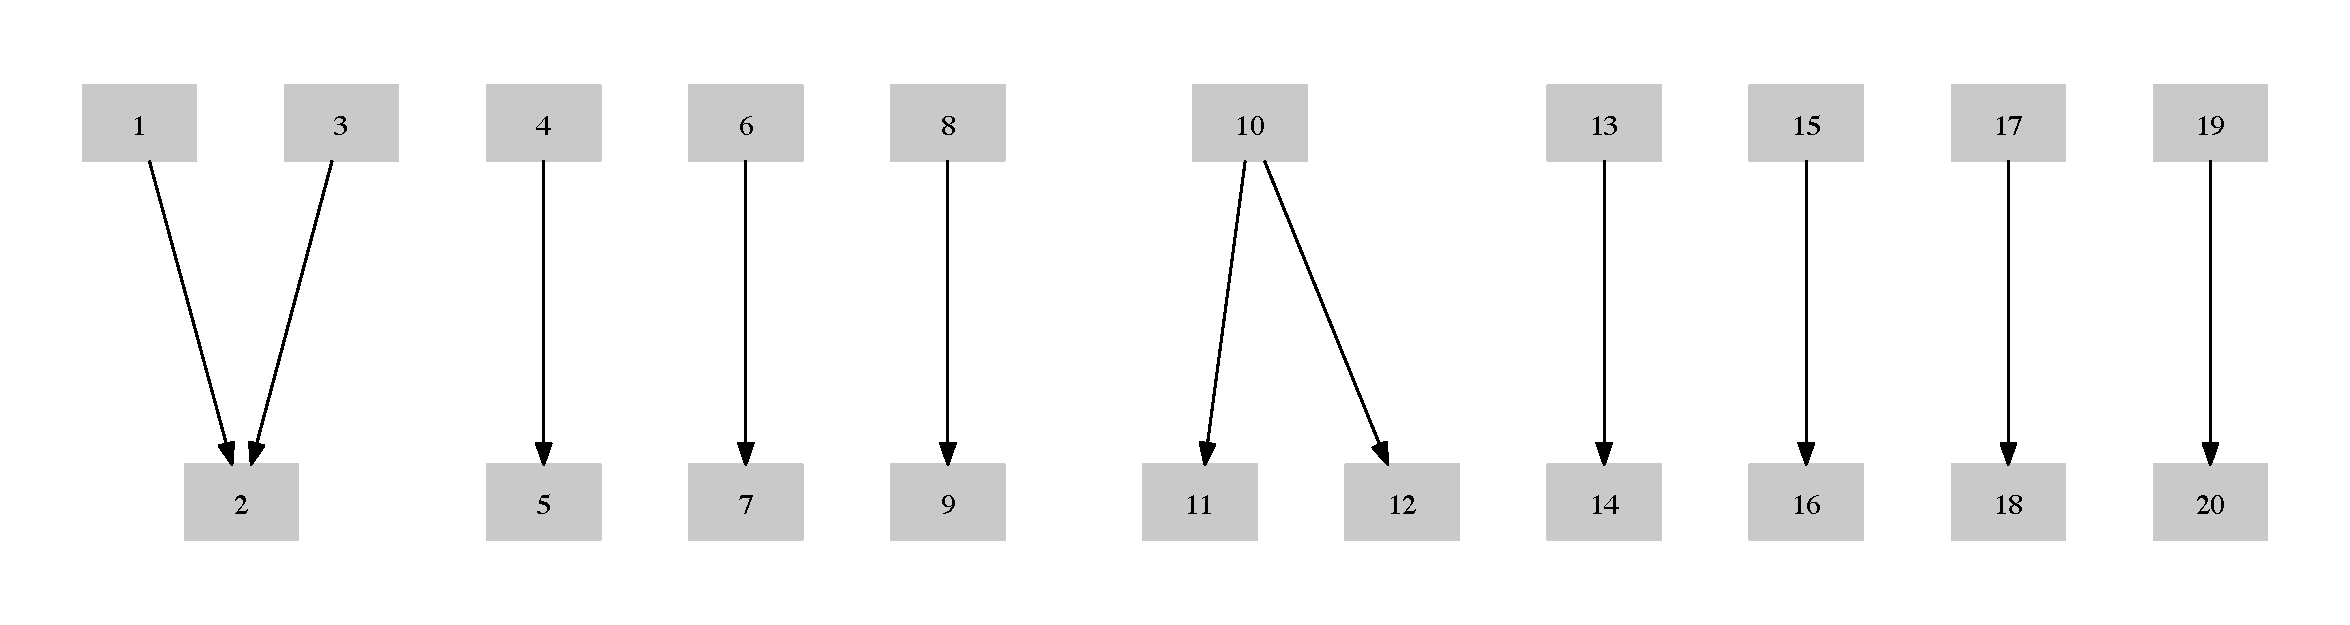
\includegraphics[width=1\textwidth]{images/from-network-connections.pdf}
  \end{center}
  \caption{Dependency graph: Graph from network connections, resulting from execution in the case study. Application names are masked.}
  \label{fig:graph_from_network}
\end{figure}

\subsubsection{Discussion}

Given the resulting graph in \ref{fig:graph_from_network} we can see that only few applications and dependencies were identified. Also these are not well-connected. We conclude that at least the graph we created in the case study is not a satisfying representation of the actual state of the architecture we investigated.

A major problem with this method is identifying the source application of a connection. In our case study investigation, we used an implementation detail of Bazooka to collect the information. This appears to be a brittle approach since there are no guarantees that this implementation detail might not change in future versions of Bazooka. It also is not possible to use the approach when other systems than Bazooka are used for deployment.

An easier problem to solve was mapping the destination application of a connection, given that we assume mechanisms for reverse service discovery to exist. During our investigations we were able to only resolve a small subset of destination applications (11 from 260). We attribute these to a low adoption of Glimpse. We also did not take ``Semantic DNS CNAMEs'' into consideration, which in earlier \nref{subsec:graphfromdeploymentconf} made up for a significant share of services.

% As impeding factors we see a low adoption of Glimpse in our case study, as well as the fact that applications deployed on Bazooka typically mostly have application dependencies on backing applications, which in turn are stateful and thus not deployed with Bazooka. In our case study, these applications are not part of service discovery, but usually identified via their physical hostnames. We think, that it is possible to have all deploys under service discovery, which then would then also allow inverse service discovery for all destination application. The exception might be applications that are outside of the organization's boundary, for example external REST APIs.

In our case study implementation, we probed for current connections at regular intervals. Therefore, we are not able to detect connections that did not happen at the times of probing. Examples might be application dependencies that have low traffic or only have traffic during certain times. The probability of detecting all connections increases if measurements are done over a longer time period.

% Given this would measure for a very long time, depending on the rate of change between application dependencies, it might capture too many dependencies. For example if application A has a dependency to database B, but then changes that to a dependency to database C, if the measurement was executed over the length of the change, the dependencies to both databases would be visible in the graph.

We measured connections on all Bazooka application hosts. Depending on the number of hosts, this might be a substantial effort, with regards to orchestration of the measurement and impact on the running system. Also, the measuring itself might create big data volumes to be analyzed. These might be handled by analyzing the connections immediately and aggregating the results on the machine.

One problem we did not investigate are networking mechanisms like network address translation or proxy servers. Since these effectively hide the true origin IP address, they might impede on the possibility for reverse service discovery.

To conclude, we have shown that this method is \textbf{feasible}, even though in our case study we only detected a subset of the application dependencies. The  \textbf{correctness} of the method depends on the mechanism to detect connections, as well the mechanisms for mapping source and destination IP addresses and ports reliably to application identifiers. In our case study, we have shown that it is possible to execute the method in an \textbf{automated} way.

\subsubsection{Future Work}

% We have found the mapping of source applications to be a major problem of the method. Next, we will introduce some options for future investigations:
%
% A more structured way would be to implement the functionality with the Bazooka Repository Manager, as a well-defined API. Holds true for
%
% Different ways of mapping source applications. A suggestion would be Port ranges? Then possible to do

To measure connections, another option to investigate is measuring on the network directly. Networking equipment like switches do allow to the monitoring of connections and packets \cite{Hogg}. The problem here is deriving the source application, which in our case study involved knowledge that only exists on the applications hosts, thus making network capturing infeasible. Instead of the network, communication might also happen via other media. An example is the ``Service Bus'' in SOA as explained in \cite{enterpriseSOA} section 4.3.4.

We also see three options for future work regarding ``reverse service discovery'':
\begin{titemize}
  \item In earlier \ref{subsec:graphfromdeploymentconf}, we introduced the ``reverse service discovery'' method \emph{Semantic DNS CNAMEs}. We did not use this method in the case study execution here but believe that it might improve the results significantly.
  \item More work can be done in exploring how to map IP addresses to application names. For example Chef might be used, in the same way as already explained in earlier \ref{subsec:graphfromdeploymentconf}.
  \item Packet inspection could be used to identify source applications. For example, the packet content could be annotated with the source application identifier. A practical implementation could be using the HTTP protocol with a custom header holding that information. This is similar to the way tracing frameworks work, which we will introduce in the following section \ref{section:graph_future_work}.
\end{titemize}

\section{Discussion}

We introduced four methods for generating an application dependency graph from a deployed microservice architecture.
\begin{tdescription}
  \item[\ncref{subsec:graph_manual_annotation}] We found this method to be the most complete and correct method. We showed that it is feasible to execute this method within an organization. By its nature, this method is only semi-automated. The gathering of annotations and graph generation may be automated. The creation and maintenance of dependency information is manual.
This impedes on the feasibility of the method (due to lack of knowledge with the executing people) and the correctness (due to lack of knowledge with the executing people, differing willingness of people in the organization to create annotations, continuous effort to adapt annotations to change in architecture).
  \item[\ncref{subsec:from_smi}] We found the assumptions of this method not to be fulfilled in our case study. To correctly identify internal application dependencies, these would have to be deliberately encapsulated, which appears to be a significant change to existing codebases. Also, the problem of mapping module names to application dependencies seems to only be solvable by manual mappings. We conclude that this method might be feasible, but would demand significant effort to change existing structures.
  \item[\ncref{subsec:graphfromdeploymentconf}] We found this method to be feasible and potentially providing correct results. The execution of the method can be automated. In the case study execution, we found that only some service dependencies could be mapped to application identifiers, since reverse service discovery was not always possible. Also we only investigated deploys done with the \emph{Bazooka} deployment system, thus we did not capture all deployed applications.
  \item[\ncref{subsec:from_network}] We found this method to be feasible within our case study. Problematic was mapping the applications, which limited the method in our investigations.
\end{tdescription}

Since in our case study only \ncref{subsec:graph_manual_annotation} gave us a complete picture of the architecture, we will continue using the dependency graph we constructed from our case study with that method in the following chapters.

We did an informal qualitative evaluation of that graph with engineers of the case study company. A common reaction was to search for the applications the particular engineers were concerned with in their daily work. From there they analyzed and discussed incoming and outgoing edges. It occurred that existing edges were surprising to engineers and showed unexpected dependencies. Circular dependencies were a topic of concern for engineers, which were identified and discussed with the help of the dependency graph. A common concern for the dependency graph was as to which extent it represents the currently deployed architecture. We also learned that other engineers in the past tried to create similar graphs manually. They never created a meaningfully complete graph of all applications, but rather either only looked for a small subset, usually from the perspective of one application or they made a high-level architecture diagram which did not follow a consistent or holistic entity model. Other architecture overviews we encountered were data flow diagrams and request flow diagrams. Both were usually based on actual deploys of applications and only featured a limited subset of the architecture.

We believe that \ncref{subsec:graphfromdeploymentconf} and \ncref{subsec:from_network} are feasible automated ways to generate application dependency graphs and might be fruitful for future work. They both make assumptions towards the infrastructure tooling, especially with regards to reverse service discovery. It is to be investigated, how these can be satisfied without compromising other requirements, like low system complexity or scalability.

A problem with all methods was to distinguish applications that are currently deployed in the production deployment environment. We proposed criteria for manually filtering applications in manual creation (among them excluding infrastructure, deprecated and prototype applications). The same criteria were then used for manually filtering applications in the other methods as well. With all methods we hoped to find ways of running them highly-automated, but eventually did not succeed in doing so. All methods needed manual intervention at some point, for example when filtering for applications and deploys that are part of the production deployment environment.

If microservice architecture continue to grow in popularity, we expect ``programmable infrastructure'' to become more prevalent. We see programmable infrastructure as the attribute of systems to enable the planning, creation, maintenance and monitoring of an architecture. These systems will then also allow programmable interaction, which in turn allows for more sophisticated analysis of the architecture, just as we have executed them in this chapter.

% PaaS is awesome
% In our investigations, we have seen ``programmable infrastructure'' tools (e.g. Bazooka). We see that it is beneficial to our cause to be able to have standardized ways for
% PaaS approaches and virtualization of infrastructure are likely to help lots. "Programmable infrastructure" with standardized access to all parts of the infrastructure. Currently it is "detective work" in deriving infromation from many different sources. The topology, location and the format of these data sources change over time, making human interaction needed.

% Going forward, we use the manual annotation version

% Why are we on level of application? Assumption that it is useful to argue here, since applications are natural level of abstraction from a programmers perspective. Also discussion ownership (both source code and deploy) often happens on application level. This leads to allocation of engineering time happening on the same level.

\section{Future work}
\label{section:graph_future_work}

% central overview (soa service repository, enterprise service bus
% Did AOL publish something about their infrastructure?

A method worth investigate more is deriving service dependencies from within source code. We touched onto one option for this in the ``Future work'' section of \nref{subsec:graphfromdeploymentconf}, where we proposed extracting service locations or service discovery keys from the source code. Another option would be to annotate dependencies to services in the code e.g. with a comment.

Tracing frameworks like Dapper \cite{dapper} or Zipkin \cite{zipkin} allow for collecting information on how requests travel through a system. This assumes a request/response style communication originating in one part of the system (usually the interface to the user). Each of these request gets an identifier, which is carried through the architecture when more requests are made to subsystems. This tracing information is then collected and made available for analysis. Even though initially meant for performance monitoring, tracing would also allow to extract service dependencies.

% In our work, we only investigated application dependencies that manifest via network communication. Future work could investigate other forms of application dependencies. Examples are message queues or shared data storage.

An interesting angle for future work is using a finer granularity when discovering dependencies. In our work we used applications and application dependencies. A more fine-grained approach would be by using processes. An even more detailed approach would be splitting applications or processes into functionalities and modeling dependencies between these. For example, if a service provides several HTTP resource locations, each of these could be seen as a functionality, to which other application functionality might have dependencies. Each resource location in turn would be a functionality with own dependencies. This would allow for more sophisticated dependency modeling, which in turn could also lead to new angles in dependency modeling.

\section{Summary}

The goal of this chapter was to evaluate ways of creating a dependency graph from a deployed and running microservice architecture. A dependency graph is a directed graph with applications as vertices and service dependencies as directed edges from service consumer to service provider. We proposed four novel methods for creating dependency graphs, all of which we executed in the context of our case study in a real and deployed microservice architecture. We then evaluated each method after the aspects feasibility, correctness and automation.

Of the four methods, \ref{subsec:graph_manual_annotation} manually annotating service dependencies and semi-automatically collecting these for constructing the dependency graph was the most viable option, since it provided the most complete view on the deployed architecture. The graph we constructed from our case study with that method is visible in \autoref{fig:manual_annotation_whole}.

% \item[] {\small\ref{subsec:graph_manual_annotation} \ncref{subsec:graph_manual_annotation}}
% \item[] {\small\ref{subsec:from_smi} \ncref{subsec:from_smi}}
% \item[] {\small\ref{subsec:graphfromdeploymentconf} \ncref{subsec:graphfromdeploymentconf}}
% \item[] {\small\ref{subsec:from_network} \ncref{subsec:from_network}}
%

  %!TEX root = ../master_thesis.tex

\chapter{Constructing qualitative fault trees}
\label{chapter:fault_trees}

In this chapter we describe how a dependency graph can be transformed into a qualitative fault tree. First we lay the basis for our algorithm by describing the requirements towards the dependency graph and assumptions regarding failure semantics of applications. We then describe our algorithm and finish the theory section by introducing related work. Furthermore we describe how we executed our algorithm in the context of the case study and end the chapter by discussing our findings and future work.

\section{Theory}

In this section we explain our algorithm to transform a dependency graph into a qualitative fault tree. A dependency graph is a graph representing applications as vertices and dependencies between these applications as directed edges (see earlier \nref{chapter:dependency_graph}). The algorithm has several assumptions which we will describe before we explain the algorithm itself.

\subsection{Dependency graph requirements}
\label{section:fault_tree_graph_req}

For our algorithm to work, the dependency graph has to fulfill the following requirements:

\begin{tdescription}
  \item[Directed graph] In a directed graph, all edges have a direction from a source vertex to a destination vertex. In a dependency graph, all edges fulfill this property, since dependencies between applications are directed. If this requirements is not fulfilled, our algorithm could not construct a fault tree, since it would be impossible to detect the direction of failure propagation. Interpreting undirected edges as symmetric (being directed in both directions) is not a feasible solution, since the graph needs to be acyclic, as explained next.
  \item[Acyclic graph] An acyclic graph is a directed graph which has no cycles. This means that for every vertex, if one recursively follows the outgoing edges, one will never return to the start vertex. Fulfilling this requirement in a dependency graph might be hard, since service dependencies can be cyclic. If this requirement is not fulfilled, it will not be possible to generate a fault tree with our algorithm, since the generated tree will grow indefinitely.
    \item[Rooted graph] In a rooted graph, one vertex is labeled as a special vertex, distinguishing it from others. In our case, this can be fulfilled by manually choosing a root vertex from the graph. If this requirement is not met, it is not possible to identify the vertex for the TOP event for the fault tree and therefore the algorithm can not be executed. Given a microservice architecture that implements a SaaS, interesting root vertices are applications that directly serve clients, since these represent entry points into the system.
\end{tdescription}

When executing the algorithm, it will practically be executed on a subgraph of the dependency graph, which includes all vertices and edges reached when recursively following the outgoing edges from the root vertex. It is sufficient if only that subgraph is directed and acyclic.

\subsection{Failure semantics}
\label{s:failure_semantics}

In this section we describe the assumptions about failure semantics that we base our algorithm for fault tree construction on. In short, these are as follows: 1. Applications might fail because of \textbf{internal} failures. 2. The failure of one application might \textbf{propagate} failure to all applications that depend on it. Next we will describe these assumptions in more detail.

Given that we have a dependency graph, each vertex represents one application that is part of the microservice architecture. These applications might fail individually\footnote{To be correct with the terminology from the earlier \nref{subsec:dependability_threats}, it should be ``might individually be in erroneous states, which manifest as failure events when the service is used''. For reasons of comprehensibility, we only use the terms ``fail'' and ``failure'' to refer to these cases in this section.}.

In order to exhibit a failure, the application needs to have experienced a fault. We assume that there are only two possible fault types:
\begin{tenumerate}
  \item An application might experience an \emph{internal fault}. We specify that this fault might not be because of another application's failure. Apart from that, the nature of these internal faults it not specified more here\footnote{Examples for internal faults might be design or programming mistakes when considering the application itself or failures of the execution environment. We do not consider these internal faults further in our algorithm. As future work, these could be investigated further. For example, they could be modeled with own fault trees then.}.
  \item An application might experience an \emph{external fault}. A external fault in an application A occurs, when an application B has a failure and application A has a service dependency on application B.
\end{tenumerate}

The second fault type is based on service dependencies. We defined service dependencies in earlier \nref{sec:software_environment_terminology} as the fact that application A is the service consumer of another application B, which in turn is based on the fact that one process of application A at runtime opens a network connection to a service implemented by application B.

On a more abstract note, a dependency is defined by Knight~\cite{FundamentalsDepComputing} as following: ``The dependency of system A on system B represents the extent to which system A's dependability is (or would be) affected by that of system B''. In our case we assume that the dependence between systems is very strong, leading to the immediate propagation of failures.

In practice, the dependence might not be as strong as we assume it here. Commonly fault tolerance means are used to limit the impact of dependency failures. In our concrete example this might include using spatial or temporal redundancy, or continuing in a degraded state, with some functionality of the application being disabled but others being unaffected. We explicitly do not include these means of fault tolerance in our model of failure semantics.

The practical manifestation of failures is not of concern a here. Following the failure semantic model for distributed system by Cristian~\cite{cristian}, failures could be response, timing, omission or crash failures. All result in the same failure propagation results as proposed here.

% Assumption: two failure semantics: omission failure (detected by client via timeout) or crash failure (detected by client with error response from server). In both cases it is assumed that the application does not fullfil its purpose, thus the service consumer's dependency to this application is broken. \ref{ss:failure semantics}

\subsection{Construction algorithm}
\label{subsec:fault_tree_construction}

We introduced fault trees in \nref{subsec:theory_faulttree} as a technique for structured dependability analysis. Via a graphical diagram it helps to visualize which events may contribute to a TOP event failure and how these are interrelated with each other. We described earlier that fault trees are used to comprehensively describe the causes for a TOP event failure. In this work, we limit the fault tree analysis to \emph{internal} faults in an application and \emph{propagated} faults due to failing service dependencies.

\paragraph{Algorithm}

Given that we have a rooted, directed, acyclic graph, we may construct a qualitative fault tree with the following algorithm:

\begin{tenumerate}
  \item Turn root vertex into TOP event
  \item Create OR-gate and connect it to TOP event
  \item Create basic event with name of root vertex and connect it to OR-gate
  \item Follow each outgoing edge of the \emph{current} vertex (beginning with root vertex) to the \emph{next} vertex
  \begin{tenumerate}
    \item Create intermediate event with next vertex name and connect it to OR-gate of the current vertex
    \item Create OR-gate and connect it to intermediate event
    \item Create basic event with next vertex name and connect it to OR-gate
    \item Repeat step 4 recursively for next vertex
  \end{tenumerate}
\end{tenumerate}

% \todo{introduce pruning here}

% \todo{example with three-tier web application, because everyone will be able to understand that instead of abstract example}

Figure~\ref{fig:fault_tree_graph_example} shows an example dependency graph. Vertex ``A'' is the root vertex. Figure~\ref{fig:fault_tree_graph_example_algorithm} shows each algorithm step while generating the fault tree. Since vertex ``A'' only has one outgoing edge, algorithm step 4 is executed only once for vertex ``B''. If vertex ``A'' would have more outgoing edges, algorithm step 4 would be executed for each of these. If vertex ``B'' would have outgoing edges, algorithm step 4 would be executed for each of these recursively.

It is to note that the dependency graph has the vertices ``D'' and ``E'', which we did not utilize in the algorithm execution. This is due to the fact that neither ``A'' nor ``B'' have outgoing edges to ``D'' or ``E''. Furthermore, ``D'' and ``E'' have symmetric edges and therefore form a circle. Since this does not meet our requirement of acyclicity, it is not possible to use our algorithm with them.

\begin{figure}[h]
  \centering
  \fbox{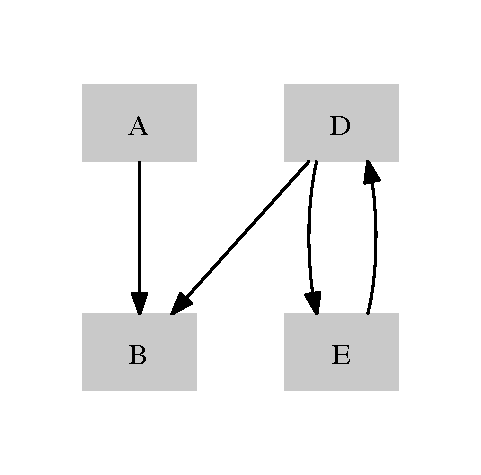
\includegraphics[width=0.4\linewidth] {images/qualitative-example/qualitative-fault-tree-example.pdf}}
  \caption{Example dependency graph for fault tree algorithm example. Root vertex is vertex ``A''.}
  \label{fig:fault_tree_graph_example}
\end{figure}

\begin{figure}[p]
  \centering
  \fbox{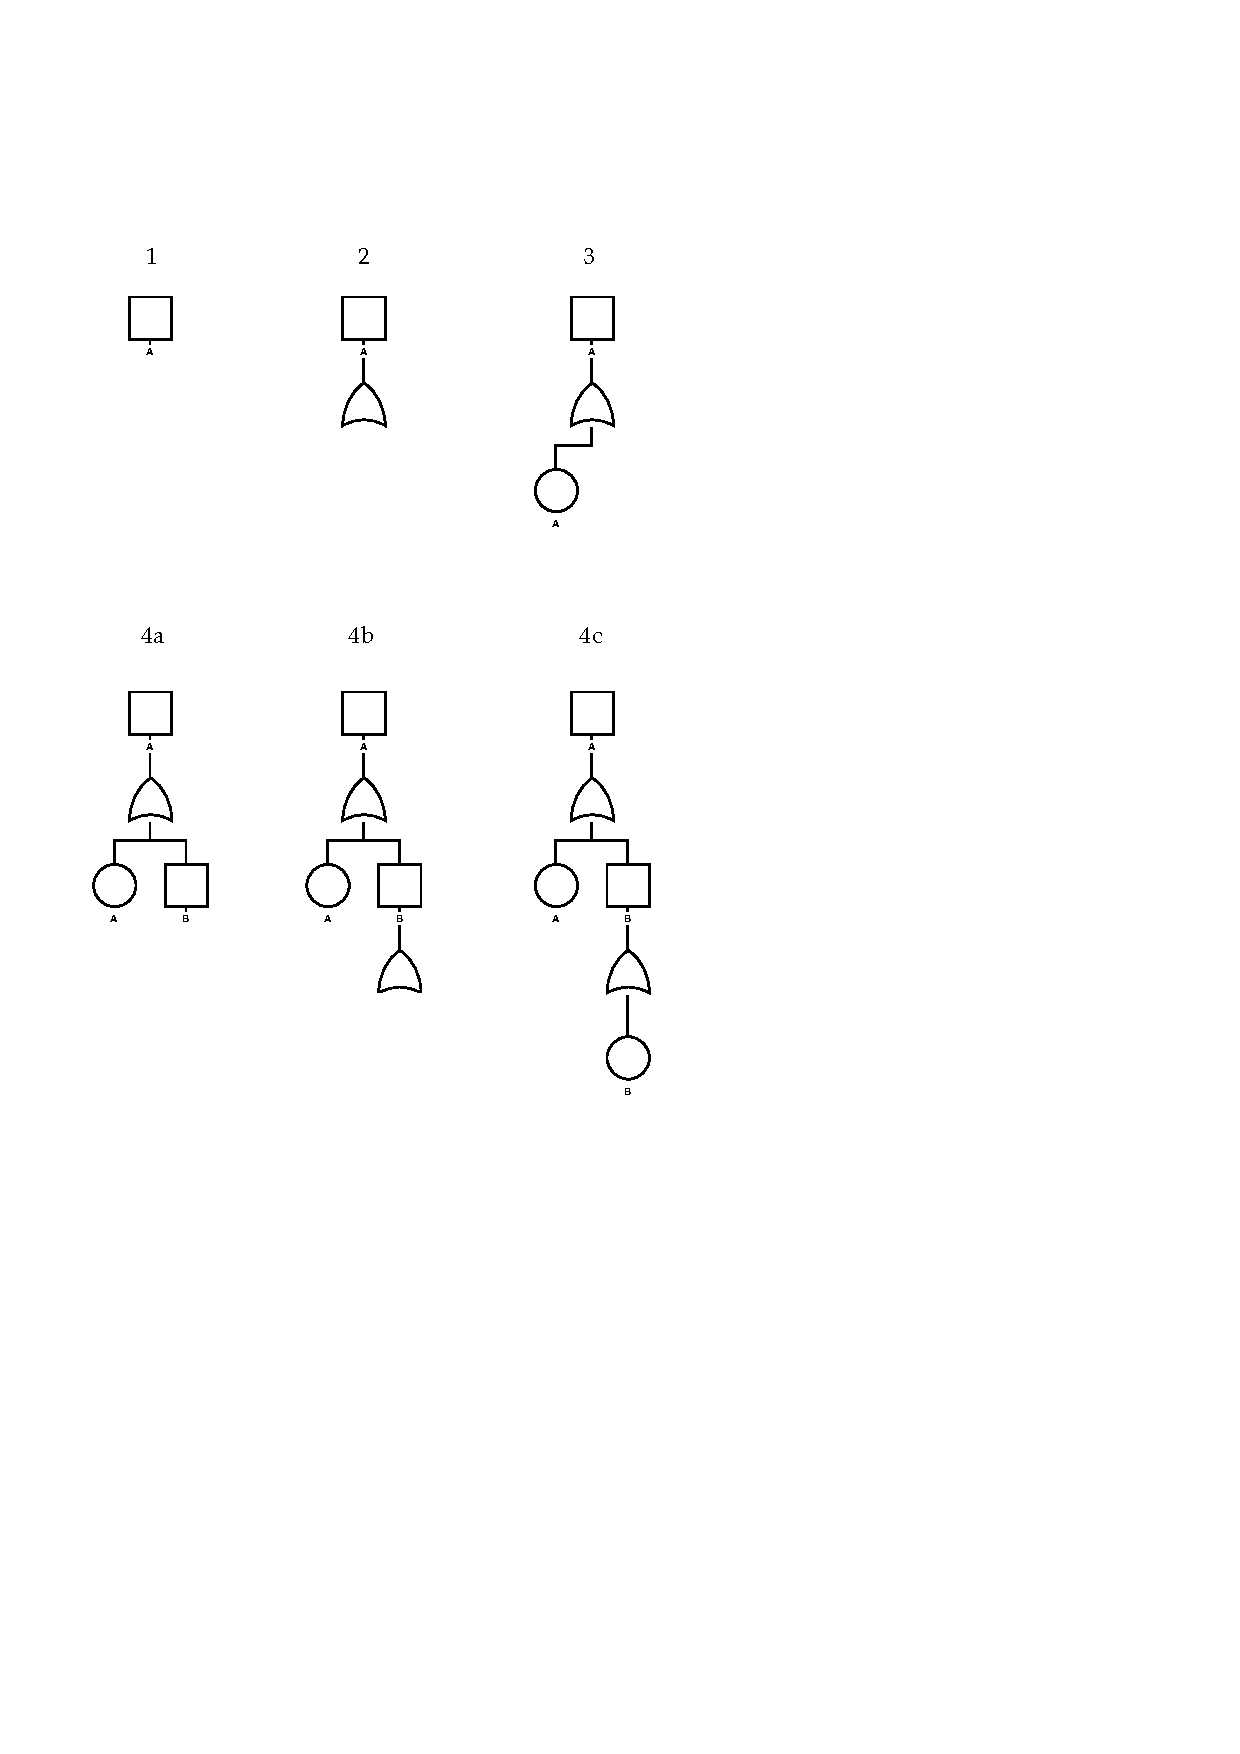
\includegraphics[width=0.9\linewidth] {images/qualitative-example/example-cropped.pdf}}
  \caption{Visualization of the algorithm for transforming a dependency graph to a qualitative fault tree. This example is based on the dependency graph in \autoref{fig:fault_tree_graph_example}}
  \label{fig:fault_tree_graph_example_algorithm}
\end{figure}

% \todo{include pruning into graph?}

\subsection{Related work}

Software fault tree analysis after Leveson et al. \cite{LevesonSoftwareFaultTrees} and Rausand et al \cite{SysReliabilityTheory} (section 4.3.8) is a software verification technique. It takes some undesired output of software as TOP event and then based on the internal structure of the software tries to derive if and how this output might occur. We do not use this technique in our work, since in our fault tree analysis we are not concerned with the internal structure of software but rather the system's view between software applications.

Lapp and Powers \cite{LAP77} proposed an algorithm for transforming directed graphs to fault trees that is similar to the one we propose here. It differs by taking more qualifying information into consideration and therefore constructing more expressive fault trees.

\section{Case study execution}
\label{sec:case_study_execution}

In this section we describe how we executed the algorithm in our case study. As basis for this we use the dependency graph in Figure \ref{fig:manual_annotation_whole} generated in \nref{subsec:graph_manual_annotation}. From that dependency graph, we chose two
root vertices to construct fault trees from: Vertex ``26'' and vertex ``73''.

% \todo{Can I rename these vertices to semantic names?}

\paragraph{Vertex ``26''} This vertex represents an application that acts as interface between the microservice architecture and the clients of the platform. Specifically, this application implements an API with the HTTP protocol, which is then used by the users' web browsers for functionality on the website \emph{\url{http://soundcloud.com}}. Therefore it does not have incoming edges, since clients (in this case browsers) are not represented in our investigation\footnote{see earlier \nref{sec:architecture} for more details}. When looking at the relevant subgraph spanning from vertex ``26'', it can be seen that there are cycles in that subgraph, revolving around vertex ``5''. We will comment in the \emph{evaluation} paragraph below on why these exist. To resolve this issue, we manually determined, which of the cyclic edges was more relevant, and removed the other edge. Figure \ref{fig:fault_tree_v2} shows the resulting fault tree for this root vertex. Please note that the fault tree is cropped, due to limitations with drawing large fault trees in the fault tree construction software we used. For reference and evaluation, Table \ref{tab:qualitative_size_comparison} shows statistics over the size of the fault tree with comparison to the size of the dependency graph it was based on. A second note is that for technical reasons the naming of the vertices in \autoref{fig:manual_annotation_whole} does not coincide with the naming of events in \autoref{fig:fault_tree_v2}.

% https://fuzzed.org/editor/932
% /Users/johan/Code/go/src/github.com/freenerd/thesis-tools/fuzzed/arch-all-masked-v2.graphml
\afterpage{%
\thispagestyle{empty}
  \begin{figure}[t]
    \vspace*{-0.9cm}
    \centering
    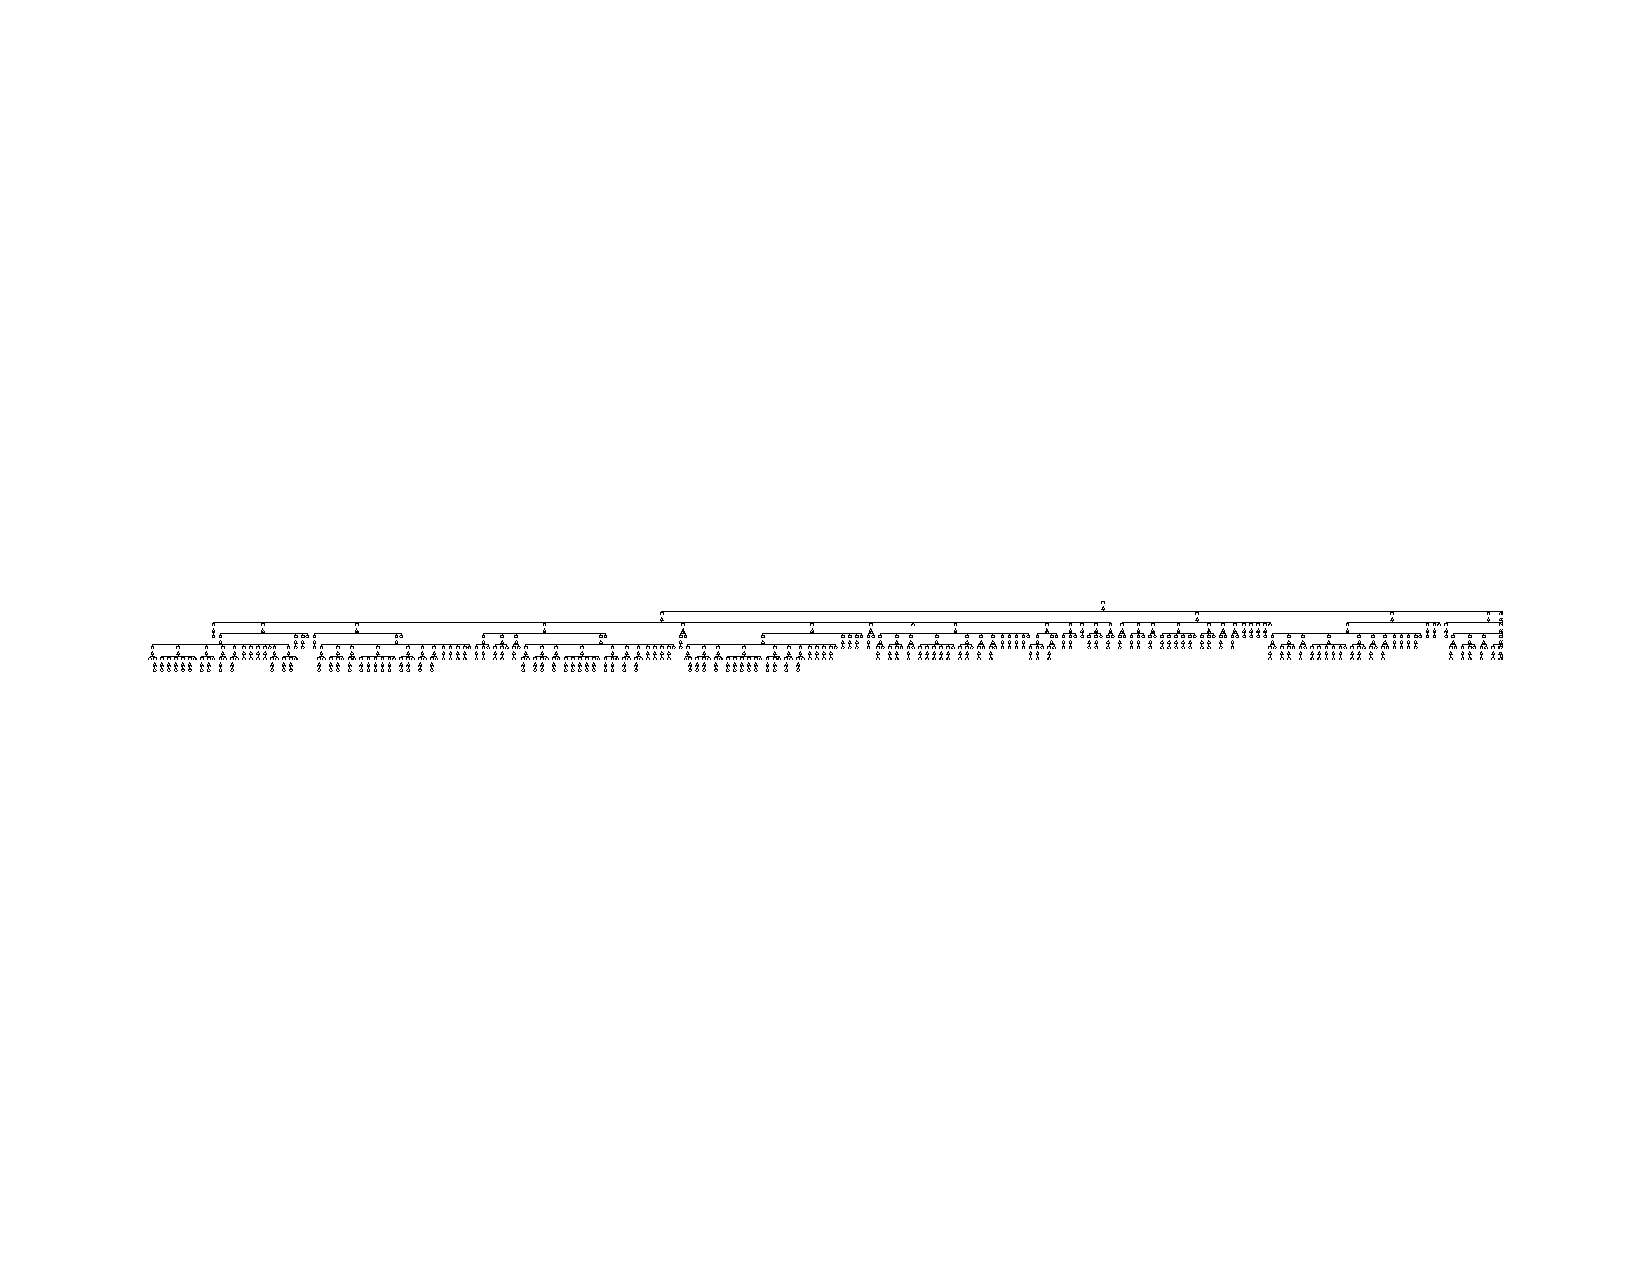
\includegraphics[angle=90, width=0.14\linewidth] {images/qualitative-fault-tree-v2-cropped.pdf}
    \caption{Qualitative fault tree for vertex ``26'' from case study dependency graph figure \autoref{fig:manual_annotation_whole} (cropped)}
    \label{fig:fault_tree_v2}
  \end{figure}
\clearpage
}

\paragraph{Vertex ``73'' (threaded-comments)} Similar to previous vertex ``26'', vertex ``73'' represents an application that exposes an API with the HTTP protocol to users' internet browsers. Therefore its vertex does not have incoming edges in our microservice architecture. We chose this vertex because we were interested in using a small subgraph for investigations in the following \nref{chap:quantitive_fault_tree}. For better visibility, we visualized the subgraph for vertex ``73'' in \autoref{fig:dep_graph_threaded_comments}. The vertices of the subgraph carry the original unmasked application identifiers as were assigned in \nref{subsec:graph_manual_annotation}. When extracting this subgraph, we made one major simplification: We did not include the outgoing edges for the vertex ``5'' in the dependency graph respectively application ``github.com/soundcloud/soundcloud'' in the subgraph. Our intention was to keep the subgraph small, in order to allow for further investigation in \nref{chap:quantitive_fault_tree}. We were not able to find another suitable subgraph which would allow these investigations without making the simplification we did here. The fault tree resulting from executing our algorithm on the subgraph can be seen in \autoref{fig:fault_tree_threaded_comments}.

\begin{figure}[h!]
  \centering
  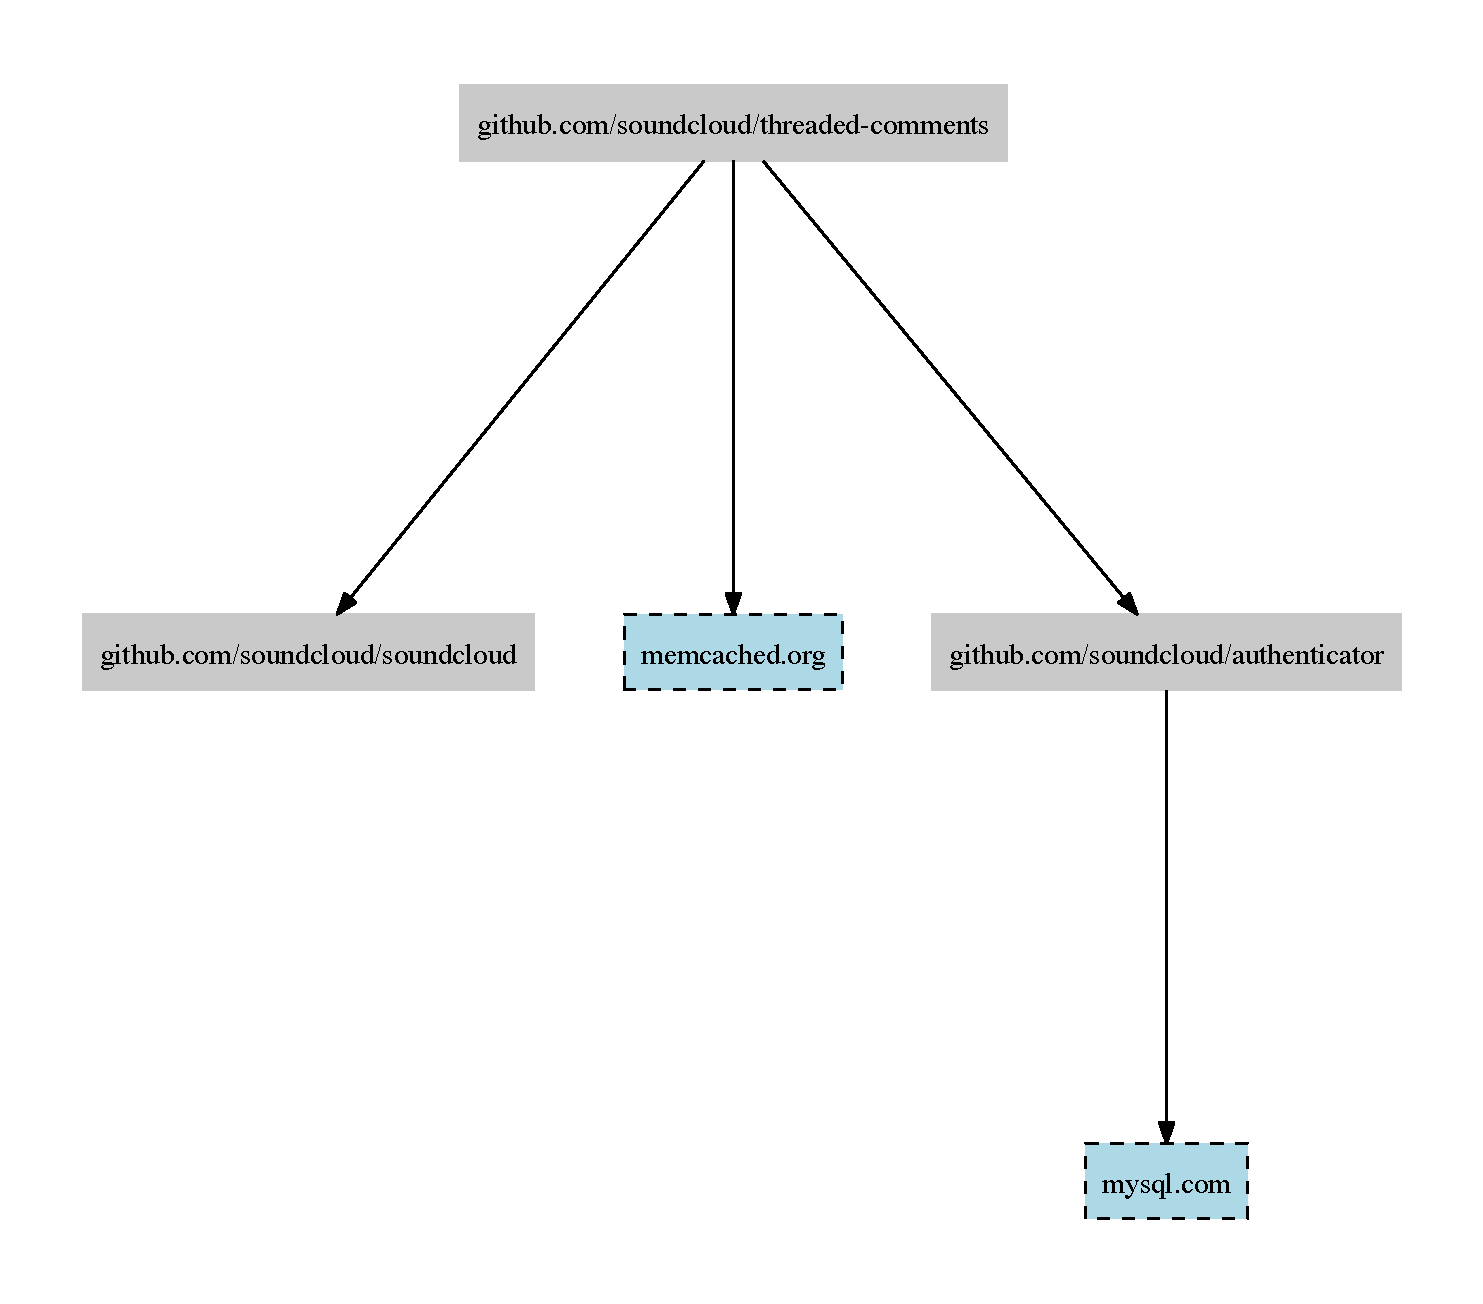
\includegraphics[width=0.6\linewidth] {images/dependencies-threaded-comments.pdf}
  \caption{Subgraph for vertex ``73'' from case study figure \autoref{fig:manual_annotation_whole}. The outgoing edges for vertex ``5''/application ``github.com/soundcloud/soundcloud'' have been removed. The vertex names have been unmasked to carry their original application identifiers.}
  \label{fig:dep_graph_threaded_comments}
\end{figure}

\begin{figure}[h!]
  \centering
  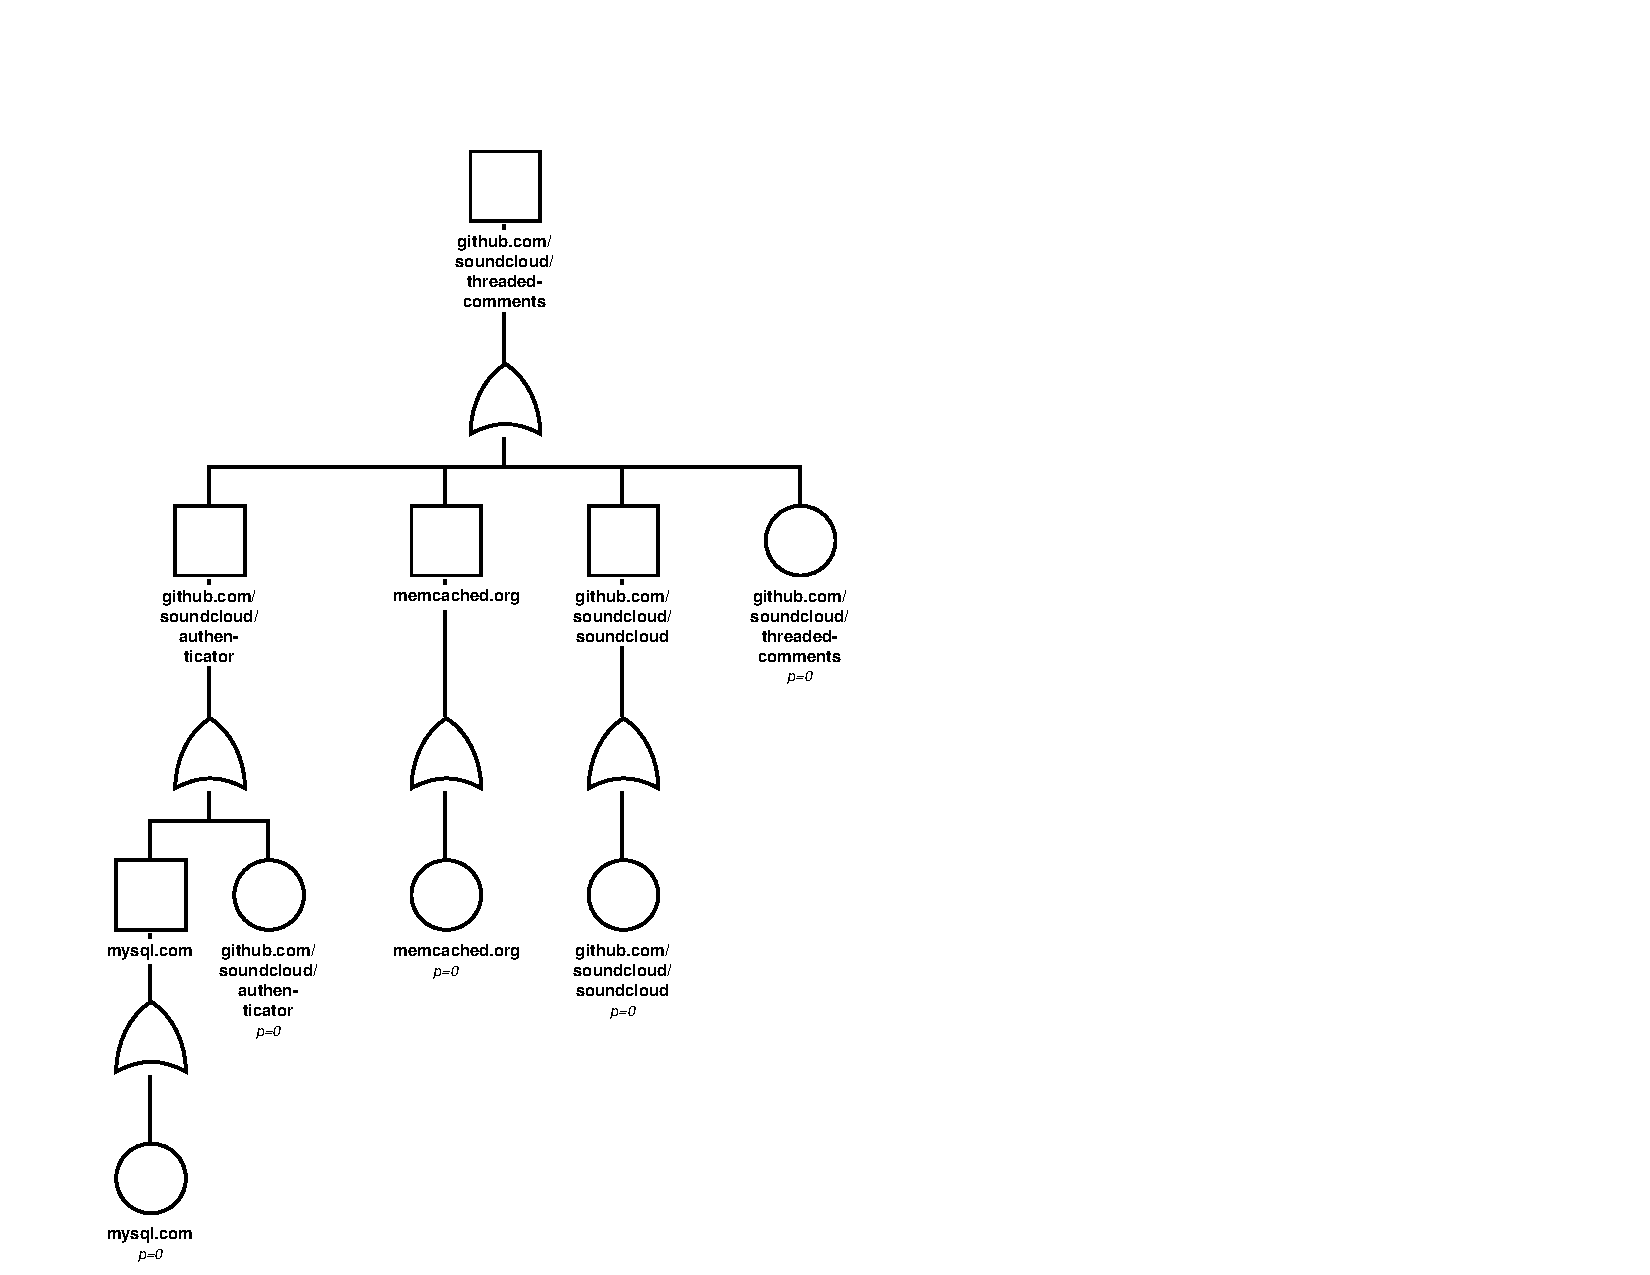
\includegraphics[width=0.6\linewidth] {images/threaded-comments-fault-tree-cropped.pdf}
  \caption{Qualitative fault tree for vertex ``73''/application ``github.com/soundcloud/soundcloud'' following the dependency graph from \autoref{fig:dep_graph_threaded_comments}.}
  \label{fig:fault_tree_threaded_comments}
\end{figure}

Please note that for brevity in this work, we have shortened the application identifiers as shown in \autoref{tab:shortened_app_names}. Furthermore, \autoref{tab:app_name_descriptions} shows descriptions for the applications involved.

\begin{table}
  \caption{Shortened application identifiers of subgraph for vertex ``73'' shown in \autoref{fig:dep_graph_threaded_comments}.}
  \label{tab:shortened_app_names}
  \begin{tabular}{ |l|l| }
    \hline
    Full application identifier & Shortened application identifier \\
    \hline
    github.com/soundcloud/soundcloud & soundcloud \\
    github.com/soundcloud/threaded-comments & threaded-comments \\
    github.com/soundcloud/authenticator & authenticator \\
    mysql.com & mysql \\
    memcached.org & memcached \\
    \hline
  \end{tabular}
\end{table}

\begin{table}
  \caption{Description of applications of subgraph for vertex ``73'' shown in \autoref{fig:dep_graph_threaded_comments}.}
  \label{tab:app_name_descriptions}
  \begin{tabular}{ |l|l| }
    \hline
    Shortened application identifier & Description\\
    \hline
    soundcloud & Former-monolithic main business logic application \\
    threaded-comments & Application to group and cache comments \\
    authenticator & Authentication and authorization of requests \\
    mysql & Relational database \\
    memcached & In-memory key-value, used as cache store \\
    \hline
  \end{tabular}
\end{table}

\section{Discussion}

As we have seen with \autoref{fig:manual_annotation_whole} and \autoref{fig:dep_graph_threaded_comments}, it is possible to generate fault trees from dependency graphs with our algorithm. In this section we will discuss these and the algorithms.

The most notable fact of our algorithm is that it only uses OR-gates as logic gates. This leads to the fact that each basic event is a minimal cut set and therefore each basic event is a ``single point of failure'' for the TOP event. As a result of this fact, employing analytical methods that are based on cut set analysis will yield low insights. We believe that the architecture of the system is not holistically expressed in the generated fault tree, since all basic events have the exact same influence on the TOP event. As major reason for that structure we see the exclusion of fault tolerance in the construction process. We will discuss opportunities for including these during automatic execution in the following future work section.

Table \ref{tab:qualitative_size_comparison} shows the sizes of the dependency graphs and the fault trees that our algorithm generated for them. It can be seen that the fault trees have magnitudes more elements and edges than the dependency graphs. One reason for the size increase is the duplication of dependency subgraphs in the fault tree: If a vertex has several incoming edges, the subgraph spanned by its outgoing edges will be present several times in the fault tree, since it will be duplicated for each incoming edge. Another reason for the size increase is the usage of intermediate events and logic gates, which are not necessary in the dependency graph.

% ~GOPATH/src/github.com/freenerd/thesis-tools/graphs/cat arch-all-masked.dot (look for biggest number)
% ~GOPATH/src/github.com/freenerd/thesis-tools/graphs/cat arch-all-masked.dot | grep "\->" | wc

% cat ~GOPATH/src/github.com/freenerd/thesis-tools/fuzzed/arch-all-masked-v2.graphml | grep edge | wc
% ~GOPATH/src/github.com/freenerd/thesis-tools/fuzzed/cat arch-all-masked-v2.graphml | grep "basicEvent" | wc
%

One of the assumptions of our algorithm is that there are no circles in the graph. As we have seen in the case study, circles do appear in reality, which hinders using the algorithm. We manually resolved the dependencies in the case study, which we believe is a poor solution.

We believe that for an engineer to get an overview over the architecture, dependency graphs are better suited than fault trees, due to their significantly smaller size. We see potential in improving the algorithm as explained in the following Future work section. We also see potential of the fault trees as basis for quantitative fault trees, as explained in the following \nref{chap:quantitive_fault_tree}.

\vfill\clearpage

\begin{table}[!ht]
  \caption{Sizes of dependency graphs and the generated fault trees}
  \label{tab:qualitative_size_comparison}
  \begin{tabular}{ |l|l| }
    \hline
    \multicolumn{2}{|l|}{Dependency graph with root vertex ``26'' (not visualized)} \\
    Vertices & 49 \\
    Edges & 97 \\
    \hline
    \multicolumn{2}{|l|}{Fault tree for vertex ``26'' \autoref{fig:manual_annotation_whole}} \\
    Elements & 1146 \\
    Basic Events & 382 \\
    Edges & 1145 \\
    \hline
    \multicolumn{2}{|l|}{Dependency graph with root vertex ``73'' \autoref{fig:dep_graph_threaded_comments}} \\
    Vertices & 5 \\
    Edges & 4 \\
    \hline
    \multicolumn{2}{|l|}{Fault tree for vertex ``73'' \autoref{fig:manual_annotation_whole}} \\
    Elements & 15 \\
    Basic Events & 5 \\
    Edges & 14 \\
    \hline
  \end{tabular}
\end{table}

% On the bottom are backing applications. They provide a service, but don't consume one themselves. Typical examples are data storage systems.

\section{Future work}

In the discussion we have seen that the size of the fault tree is problematic. We see two opportunities for future work to improve on that:
\begin{titemize}
  \item To reduce the number of elements and edges in the fault tree, we see the following simplification: All vertices with no outgoing edges will follow the same pattern of being represented by one intermediate event, one OR-gate and one basic event. These can be compacted by removing the intermediate event and OR-gate, and connecting the basic event directly to the parent OR-gate.
  \item We have discussed that the same subgraph may appear several times in the fault tree. To improve on that, a ``Transfer In'' element\footnote{A ``Transfer In'' element is a fault tree element that allows to include another fault tree. The ``Transfer In'' element then represents the TOP event of the included fault tree.} may be used.
\end{titemize}

The fault trees our algorithm generated are limited to OR-gates as logic gates only. This limits the applicability of analytical methods based on cut sets. Thus the goal of future work should be to improve the expressiveness of the fault tree. Next we will introduce several opportunities for that:
\begin{tdescription}
  \item[Manual extension] The generated fault tree could be taken as a basis for manual extension by engineers. Examples for extensions are including runtime environments of applications, non-technical influences like human interaction, or the methods introduced below.
    \item[Application fault tolerance] Future work should investigate representing fault tolerance of applications in the fault trees. Examples for application-internal fault tolerance mechanisms to investigate are temporal and spatial redundancies (which might result in using AND-gates or K/N-gates in the fault tree) as well as degraded service (which might allow for splitting applications into finer-grained functionalities).
    \item[Different application granularity] In earlier \nref{section:graph_future_work} for generating dependency graphs, we already discussed potential for different granularities for applications. These might be deploys, processes or functionality. Each of these would allow different algorithms, which in turn would result in different fault trees. These could aid the expressiveness of the fault tree.
    \item[Infrastructure applications] In our investigations, we did not take infrastructure applications (like deployment systems or traffic management systems) into consideration. Future work could investigate how to include these in the algorithm. This would improve the scope of the fault tree in the direction of a more holistic view. It might also help to model system fault tolerance, since it is sometimes realized through infrastructure applications (e.g. load balancers).
\end{tdescription}

\section{Summary}

In this chapter we suggest qualitative fault trees as a way of modeling failure propagation in microservice architectures. We proposed a novel algorithm for transforming dependency graphs into qualitative fault trees. The algorithm respects two kinds of failures: internal failures from applications themselves and external failures propagating through the architecture via service dependency failures. Fault tolerance mechanisms were not considered. We executed the algorithm for one application of the case study's dependency graph with the resulting qualitative fault tree visible in \ref{fig:fault_tree_threaded_comments}.
  %!TEX root = ../master_thesis.tex

\chapter{Constructing quantitative fault trees}
\label{chap:quantitive_fault_tree}

Based on the qualitative fault tree structure, we would like to quantify the failure probabilities of the basic events to calculate the probability of the TOP event. The actual TOP event probability itself may not be useful in assessing the dependability of a system. But it is possible to evaluate how changes to basic event probabilities affect the probability of the TOP event.

We base our investigation in this section on the fault tree from previous \nref{subsec:fault_tree_construction}, specifically shown in \autoref{fig:fault_tree_threaded_comments}.

To calculate the probability of the TOP event, we use the transformation rules as described earlier in \nref{subsec:theory_faulttree}, resulting in the following equation:

% \autoref{eq:quant_bool} shows the fault tree as a boolean logic equation:
%
% \begin{multline} \label{eq:quant_bool}
%    Top Event = \\
%       \shoveleft{( \operatorname{mysql} \vee \operatorname{authenticator} ) \quad \vee} \\
%       \shoveleft{\operatorname{memcached} \quad \vee} \\
%       \shoveleft{\operatorname{soundcloud} \quad \vee} \\
%       \shoveleft{\operatorname{threaded-comments}}
% \end{multline}

% \autoref{eq:quant_prob} shows the boolean logic equation from previous \autoref{eq:quant_bool} tranformed to an equation for calculating the top event probability.

{\scriptsize
\begin{multline} \label{eq:quant_prob}
  P(TOP Event) = \\
     \shoveleft{P(mysql) + P(authenticator) - P(mysql) * P(authenticator) +} \\
     \shoveleft{P(memcached) -} \\
     \shoveleft{(P(mysql) + P(authenticator) - P(mysql) * P(authenticator)) * P(memcached) +} \\
     \shoveleft{P(soundcloud) - }\\
     \shoveleft{(P(memcached) - (P(mysql) + P(authenticator) - P(mysql) * P(authenticator))} \\
     * P(memcached)) * P(soundcloud) + \\
     \shoveleft{P(threaded\mbox{-}comments) -} \\
     \shoveleft{(P(soundcloud) - (P(memcached) - (P(mysql) + P(authenticator) - P(mysql) * P(authenticator))} \\
     * P(memcached)) * P(soundcloud))) * P(threaded\mbox{-}comments)
\end{multline}
}

\clearpage

To solve the equation probabilities for all basic events are needed. Rausand et al~\cite{SysReliabilityTheory} (section 4.3.5) introduce three categories for approaches for handling probabilistic analyses of software failure. All of these assume a fault tree that includes software, hardware and other events.
\begin{tenumerate}
  \item \textbf{Assume the probability of software failure is zero} This approach assumes that software never fails. It therefore limits the probabilistic analysis to the other components. We use this approach for software components that the deployed method may not derive probabilities for, therefore we set these probabilities to 0.
  \item \textbf{Assume the probability of software failure is one} This approach assumes that software always fails. It is therefore very pessimistic, since even though we may assume that software will eventually fail, usually it is more dependable than that. We do not use this approach in our works.
  \item \textbf{Separate the analysis of the software} This approach proposes to use separate analysis methods for software and other components. The methods we propose here may be seen in the context of this category.
\end{tenumerate}

For assessing the basic event probabilities we investigated the following methods:
\begin{tenumerate}
  \item Source code metrics
  \begin{tenumerate}
    \item Lines of code
    \item Code churn
  \end{tenumerate}
  \item Operational availability
  \begin{tenumerate}
    \item External heartbeat measurements
    \item Production traffic measurements
  \end{tenumerate}
\end{tenumerate}

We executed each of these methods in the context of our case study. Please note that a quantitative analysis of the methods was out of scope for this work. We executed the methods to show their feasibility. We do however evaluate each method qualitatively.

\section{Via source code metrics}
\label{sec:source_code}

Source code metrics provide insights about the state of a software by analyzing source code and its meta data. In this section we describe two methods for deriving failure probabilities from source code metrics. For each method we explain how we executed it in our case study and discuss its results.

\subsection{Lines of code}
\label{subsec:loc}

The \emph{lines of code} (short: \emph{LOC}) of an application are all text lines that contribute to the codebase of it. Earlier in \nref{sec:software_environment_terminology} we assumed that each application has exactly one codebase and that we are able to map the application identifier to its codebase. In our case study this assumption is true for internal applications, but not for external applications. Thus we manually linked the external application identifiers to the appropriate codebases.

We manually acquired the codebases for each application in the fault tree. We then counted the lines of code for each codebase. Our measurement of LOC took all lines of text in the codebase into consideration. This included tests, deployment and build scripts, example code, documentation and comments. We did not take shared library code into consideration, except if they were included in the codebase (e.g. since they have been copied in).

The internal applications \emph{soundcloud}, \emph{threaded-comments} and \emph{authenticator} were measured with their versions from 28 April 2014. The external applications \emph{mysql} and \emph{memcached} were measured with the version numbers that were deployed in the case study on 28 April 2014. The results can be seen in \autoref{tab:loc}.

To use the lines of code in the fault tree, we have to transform them to failure probabilities. We do this based on the assumption that per 1000 lines of code (short: \emph{KLOC}), there are a number of bugs present in the code. McConnell et al \cite{McConnellSteve} surveyed papers comparing \emph{number of defects per KLOC}. The values range from 0.1 defects to 50 defects per KLOC. We optimistically chose the lower bound \emph{0.1 defects per KLOC} as ratio to estimate the number of defects in a codebase. We now have to transform these to failure probabilities, in order to use them in the fault tree. We do so by assuming that the higher number of defects has a failure probability of 0.1. We may then normalize the other defect numbers accordingly. Table \ref{tab:loc} shows the results of this method.

\begin{table}
  \label{tab:loc}
  \caption{Lines of code calculation in the case study with accompanying failure probabilities.}
  \begin{tabular}{ |l|l|l|l| }
    \hline
    Application & Lines of code & Estimated number of defects & Failure probability \\
    \hline
    soundcloud & 635436 & 63,5436 & 0,007402703 \\
    threaded-comments & 1163 & 0,1163 & 0,000013549 \\
    authenticator & 6747 & 0,6747 & 0,000078601 \\
    mysql & 8583837 & 858,3837 & 0,1 \\
    memcached & 28354 & 2,8354 & 0,000330318 \\
    \hline
  \end{tabular}
\end{table}

Given the resulting failure probabilities, we may now use these as basic event failure probabilities in earlier \autoref{eq:quant_prob} to calculate the TOP event probability. The resulting TOP event probability is \textbf{0,10704}.

\subsubsection{Discussion}

Both the functions for calculating defects per line as well as transforming defects to failure probabilities have been chosen by us as ``good guesses'', since these were not in the focus of this work. We believe that more work is needed in choosing appropriate functions and values.

Given the \emph{lines of code} numbers from table \ref{tab:loc}, we can see there is a large variance in the size of codebases in our case study. For example the \emph{mysql} codebase is more than 7000 times larger than the \emph{threaded-comments} codebase. The failure probabilities from this method are proportional to the lines of code. Therefore the calculated TOP event probability is highly influenced from the big codebases but does not respect smaller codebase well.

We calculated the \emph{lines of code} by summing up all text lines in a codebase. An opportunity for future work would be to investigate, in how much these numbers change, if only the code that is immediately used for running processes is taken into consideration.

\subsection{Relative code churn}
\label{subsec:relative_code_churn}

\emph{Code churn} is a measure based on summarizing the added and changed lines of code in a codebase for a period of time. In this subsection we will explain, how we used relative code churn to calculate the failure probability of an application.

In our case study, all internal applications' codebases were tracked in Git~\cite{ProGit}. Therefore we were able to use the approach by Kraaijeveld \cite{KaidencePost} for measuring code churn: For a git branch, gather all parent commits for the defined time period. For each commit, summarize the number of added lines. Summarize these numbers over all commits. The resulting number is the absolute code churn.

As shown by Nagappan et al \cite{Nagappan2005} relative code churn may be used as a predictor of defects in source code. Therefore, we normalize the absolute code churn by the lines of code at the time of the start of the measured period (as explained in~\cite{Nagappan2005} as measure \emph{M1}).

In our case study, relative code churn for own applications is relevant to the behavior of the deployed architecture, since deploys happen often (often within hours of the code changes being present in the codebase). We may therefore assume that the codebase's state matches the code that is deployed.

Table \ref{tab:app_churn} shows the results from calculating relative code churn over three time periods of one week, as well as over a time period of four months.

\begin{table}[!h]
  \caption{Relative code churn in the case study calculated over several time periods.}
  \label{tab:app_churn}
  \begin{tabular}{ |l|l|l|l| }
    \hline
    Application & Beginning LOC & Absolute churn & Relative churn \\
    \hline
    25 March 2014 - 31 March 2014 \\
    authenticator & 6981 & 42 & 0,006016 \\
    soundcloud & 635434 & 2478 & 0,003900 \\
    threaded-comments & 1163 & 1 & 0,000860 \\
    \hline
    01 April 2014 - 06 April 2014 \\
    authenticator & 6839 & 32 & 0,004679 \\
    soundcloud & 635571 & 326 & 0,000513 \\
    threaded-comments & 1163 & 4 & 0,003439 \\
    \hline
    18 April 2014 - 24 April 2014 \\
    authenticator & 6875 & 762 & 0,110836 \\
    soundcloud & 635165 & 893 & 0,001406 \\
    threaded-comments & 1163 & 0 & 0  \\
    \hline
    01 January 2014 - 30 April 2014 \\
    authenticator & 6322 & 3805 & 0,601866 \\
    soundcloud & 518904 & 33643 & 0,064835 \\
    threaded-comments & 1163 & 40 & 0,029235 \\
    \hline
  \end{tabular}
\end{table}

Assuming that relative code churn is a predictor for defect rates, we may also assume that it predicts the failure rates of the applications. Thus we use the relative code churn as basic event failure rates in earlier \autoref{eq:quant_prob} to calculate the TOP event probability. Table~\ref{tab:app_churn_fail} shows the results for the different time periods.

\begin{table}[!h]
  \centering
  \caption{Relative code churn in the case study: TOP event failure probabilities after the fault tree for several time periods.}
  \label{tab:app_churn_fail}
  \begin{tabular}{ |l|l| }
    \hline
    Application & Top event failure probability\\
    \hline
    25 March 2014 - 31 March 2014 & 0,010774 \\
    01 April 2014 - 06 April 2014 & 0,008610 \\
    18 April 2014 - 24 April 2014 & 0,112209 \\
    01 January 2014 - 30 April 2014 & 0,638560 \\
    \hline
  \end{tabular}
\end{table}

\subsubsection{Discussion}

We calculated the code churn for internal applications only, but did not take the external applications \emph{memcached} and \emph{mysql} into consideration. We based this decision on the fact that the deploys of both applications in our case study were not upgraded with new versions in the time of our investigation. Therefore their code churn would not influence the deployed architecture.

We base our assumptions about mapping relative code churn to defect probabilities on Nagappan et al \cite{Nagappan2005}. They investigated code churn on differences between software releases. We did our measurements in a continuous deployment environment without explicit releases. Instead of differences between releases we used arbitrary time periods to bound the code changes to include in the investigation. We did not investigate, how this change might alter the results. Future work should investigate the significance of relative code churn towards defect rates in a continuous deployment environment.

In our calculation of absolute code churn, we took into consideration all text in the codebase, regardless if it contributes to the running application. We did not evaluate how non-application text like tests, examples or documentation influence the results.

For calculating absolute churn, we did not take deleted code into consideration. This is due to the fact that in Git a modified line of code is expressed as an added and a deleted line, thus counting deleted lines would weight modified lines double and over-emphasize them against newly added lines. Furthermore we (similarly to \cite{KaidencePost}) assume that deleted code is a low-relevance churn operation.

We use relative code churn directly as failure probability. We may assume that the longer the time period for the measurement, the higher the code churn will be. This is visible in our results in \autoref{tab:app_churn}, where the relative churn numbers for weeks are magnitudes lower than the churn numbers over months. Relative code churn may then also exceed 1, when more lines have been added/changed than lines of codes existed at the begin of the time period. In that case, relative code churn could not be used anymore as failure probability directly, but would have to be normalized.

The code churn of a single application is highly influenced by the specifics of the development process used with regards to how changes to the codebase manifest themselves in the version control system. In our case study, all applications follow the same development process, loosely based on the model as outlined in \cite{GitFlow}. There, different branches (code versions) are used for developing a feature. Once the development on a feature is completed, its changes are reviewed and then merged into a central branch (example names are \emph{trunk}, \emph{stable} or \emph{master}). This branch is the one that is used while deploying. We also used that central branch for calculating code churn. Future work should investigate, to which extent other development processes influence the relative code churn and therefore the failure probabilities.

\section{Via historical availability data}
\label{sec:historical_availability}

To calculate the TOP event probability in a fault tree, we need to assign failure probabilities to the basic events. In this section we describe two methods for deriving basic event failure probabilities from historical availability data.

\subsection{Theory}
\label{subsec:historical_availability_theory}

Given that an application is deployed, we may measure the deploy's availability at runtime, which over a time period will provide us with the historical availability.

To acquire that data, we used two methods:
\begin{tenumerate}
  \item External heartbeat measurements
  \item Production traffic measurements
\end{tenumerate}

In both measurements, we derived a time series for each deploy in the production environment. Each time step in the series holds the information if the deploy was either \emph{up} or \emph{down} in that time period.

Figure \ref{fig:availability_timeseries} shows an example of such a time series. As we can see, there were two time periods where the application was successively \emph{down} (Minute 5 and minutes 9 to 10) as well as three time periods where the application was successively \emph{up} (Minutes 1 to 4, minutes 6 to 8 and minutes 11 to 12). The duration of each \emph{up} time period may also be called the \emph{time to failure}, thus the duration it took from getting to an initial \emph{up} state to the next \emph{down} state. Furthermore we may then calculate the average time it takes until failure, also called the \emph{mean time to failure} or \emph{MTTF}. Equation \ref{eq:mttf} shows how to calculate that from a time series. The execution for this with the example time series is visible in equation \ref{eq:mttf_example}.

\begin{figure}[ht]
  \centering
  
\includegraphics[width=0.7\columnwidth] {images/availability_timeseries.pdf}
  \caption{Historical availability: Example of time series for a time period of 12 minutes with \emph{1} representing ``up'' and \emph{0} representing ``down'' for the respective time step}
  \label{fig:availability_timeseries}
\end{figure}

\begin{equation} \label{eq:mttf}
  MTTF = \frac{\operatorname{Number\:of\:"up"\:steps}}{\operatorname{Number\:of\:sequences\:with\:coherent\:"up"\:states}}
\end{equation}

\begin{equation} \label{eq:mttf_example}
  MTTF_{example} = \frac{9}{3} = 3
\end{equation}

We assume that during the time of our measurement the system has reached steady-state, meaning that if we would execute the measurements over the same length but at different points in time, we would get the same MTTF value.

The software systems we investigate are by definition repairable. For example after a failure occurred a software system may continue to work as expected afterwards due to self-repair mechanisms or, if the cause of failure is a crash, by being restarted and therefore repaired externally. We work under the assumption here that these system repairs are perfect, thus that after a repair the system is ``as good as new''.

Given these assumptions, we may calculate the failure rate with equation \ref{eq:failurerate}:
\begin{equation} \label{eq:failurerate}
  \lambda = \frac{1}{\operatorname{MTTF}}
\end{equation}

As distribution for failure probability we assume an exponential distribution. Therefore the system is said to be ``without memory'': the probability of failure at any point in time is the same, regardless of the time that passed already. We may calculate the failure probability with equation \ref{eq:failureprob}:
\begin{equation} \label{eq:failureprob}
  Pr(t) = 1 - e^{- \lambda * t}
\end{equation}

The variable \emph{t} denotes the ``mission time''. Given a specific mission time \emph{t}, the probability \emph{Pr(t)} denotes the probability that the system has failed at or before that time. Intuitively we see that the longer the mission time is, the higher the probability that the system has failed will be.

Next we will describe the two methods we used for measuring the availability of systems. We executed both methods over the same period of seven days. We did not measure the applications \emph{memcached} and \emph{mysql} because no existing measuring mechanisms provided reasonable indicators for their availability.

\subsection{External heartbeat measurements}
\label{subsec:heartbeat_measurement}

To measure the availability of an application, we did regular requests to the deployed service instances of it. We will explain the method in detail next, then show our results from executing the method in our case study and end the section by discussing our findings.

\subsubsection{Measurement method}

To execute the measurements, we created our own measurement application (called \emph{measurer}). It ran on one machine within the internal network, being able to do network requests to all deployed service instances. We measured three applications: \emph{soundcloud}, \emph{authenticator} and \emph{threaded-comments}. Each application had one production deploy with many service instances. The instances were found via the Glimpse service discovery (as explained earlier in~\nref{subsubsec:glimpse}). All services used the HTTP~\cite{rfc2616} protocol. For the measurement we chose one HTTP resource for each application. \emph{Measurer} then requested that resource on all service instances of the deploy. Each HTTP request may either return an HTTP response with an HTTP status code, or may be a timeout if it has not returned after a certain period of time (in our case 30 seconds). For all resources we expected HTTP status code 200, if the call was successful. Thus, when a response with HTTP status code 200 was received, we defined that instance to be \emph{up}. If the HTTP status code was equal to or bigger than 500, or a timeout occurred, we define the instance to be \emph{down} for that period of time\footnote{During the investigations we did not receive any other HTTP status codes like 201 or 301, thus we were not concerned with them here.}.

To alleviate load and limit impact of the measurements on the running system, we only requested 10 instances of each deploy at a time, but requested all instances of each deploy eventually within one measurement step. In \autoref{fig:heartbeat_duration} are the total durations for querying all instances of an application in each measurement runs. For \emph{authenticator} and \emph{threaded-comments}, these always finished quickly. For \emph{soundcloud} these show some spikes, resulting from some requests timing out at the 30 second mark we set as timeout interval.

\begin{figure}[ht]
  \fbox{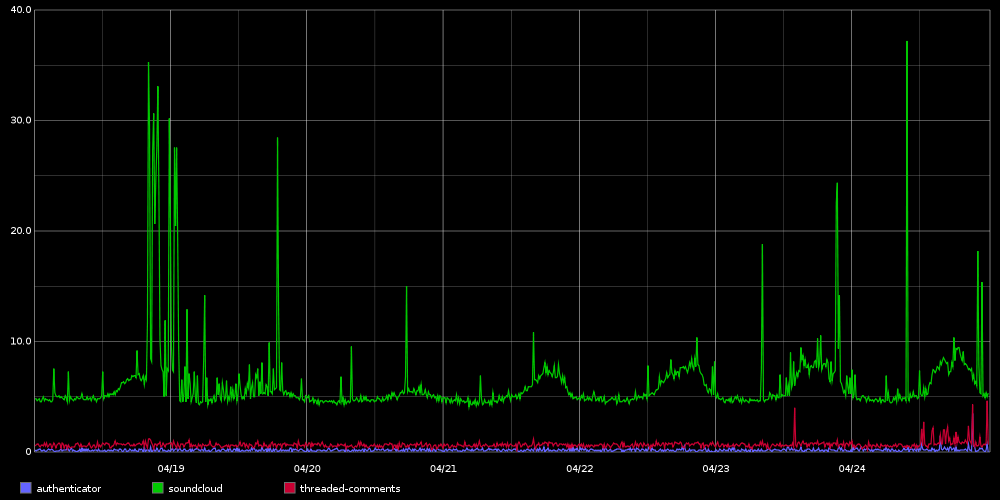
\includegraphics[width=\columnwidth] {images/availability/apr18/durations.png}}
  \caption{Heartbeat measurement: Duration of each measurement step for each application}
  \label{fig:heartbeat_duration}
\end{figure}

One measurement happened every minute. The measurements were executed continuously for seven days between April 18 2014 and April 24 2014 inclusively. The results were stored in a \emph{Graphite} server~\cite{graphite}, which allowed for extracting the raw time series data for further analysis but also generated the plotted visual graphs shown in this section.

\subsubsection{Results}

The results of our measurements can be seen in \autoref{fig:heartbeat_soundcloud}, \autoref{fig:heartbeat_auth} and \autoref{fig:heartbeat_tr}~\footnote{Due to the large time period represented in the plotted graphs, values are smoothed.}. Each figure holds the measurements for one application, with the responses of all instances summarized for each time period, with a plotted graph per status code. If an instance returned HTTP status code 200, we interpret that as ``\emph{instance is up}''. If an instance returned a status code in the 5XX range or the request timed out, we interpret that as ``\emph{instance is down}''. Next we will comment on each figure.

\begin{tdescription}
  \item[\autoref{fig:heartbeat_soundcloud} soundcloud] Around April 18 2014 3:00 there is an increase in \emph{200} status codes that is due to a provisioning of more instances. Around April 23 2014 14:00 there are some spikes in \emph{500/timeout}, which peak at about 30 instances.
  \item[\autoref{fig:heartbeat_auth} authenticator] Around April 22 2014 11:30 there is an increase in up and down instances. This increase is due to the experimental deployment of a development branch on one instance. The development branch was tested with different configurations against live traffic, some of which configurations did not deliver correct functionality. At April 24 2014 12:00 onwards there are occasional spikes in \emph{500/timeouts}. These peak at 2 instances and at maximum last 3 minutes.
  \item[\autoref{fig:heartbeat_tr} threaded-comments] At April 23 10:00 there is a spike of \emph{500/timeouts} that lasts for 14 minutes and peaks at 23 instances.
\end{tdescription}

\begin{figure}[ht]
  \fbox{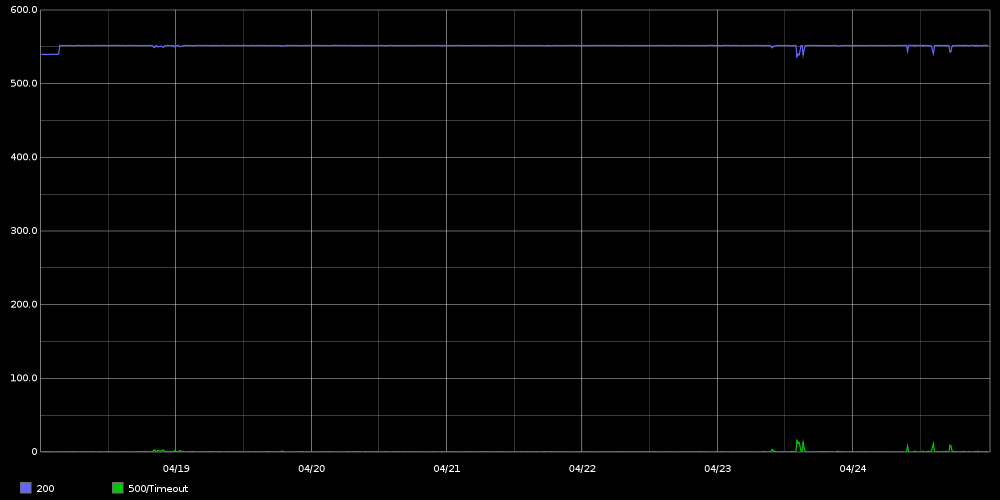
\includegraphics[width=\columnwidth] {images/availability/apr18/soundcloud_measurer_small.png}}
  \caption{Heartbeat measurement: Summarized HTTP request status codes for each measurement step for application \emph{soundcloud}}
  \label{fig:heartbeat_soundcloud}
\end{figure}

\begin{figure}[ht]
  \fbox{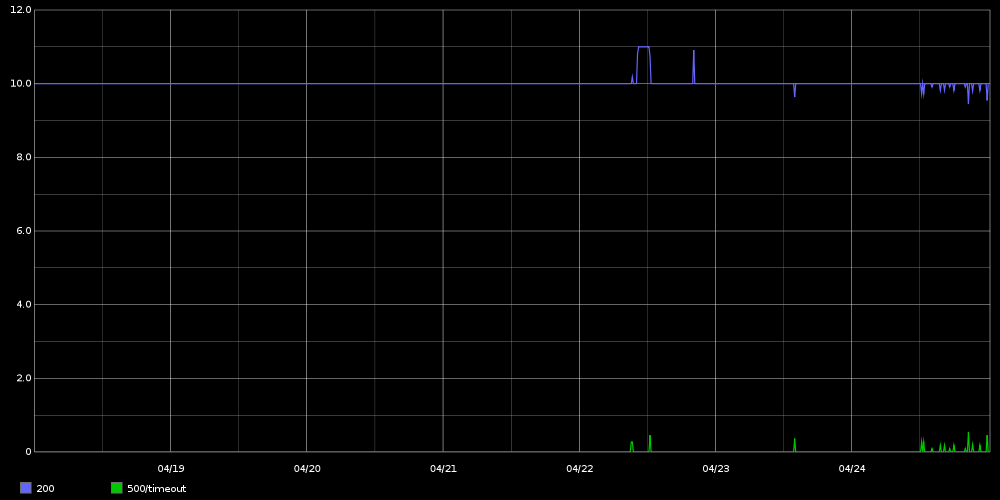
\includegraphics[width=\columnwidth] {images/availability/apr18/authenticator_measurer_small.png}}
  \caption{Heartbeat measurement: Summarized HTTP request status codes for each measurement step for application \emph{authenticator}}
  \label{fig:heartbeat_auth}
\end{figure}

\begin{figure}[ht]
  \fbox{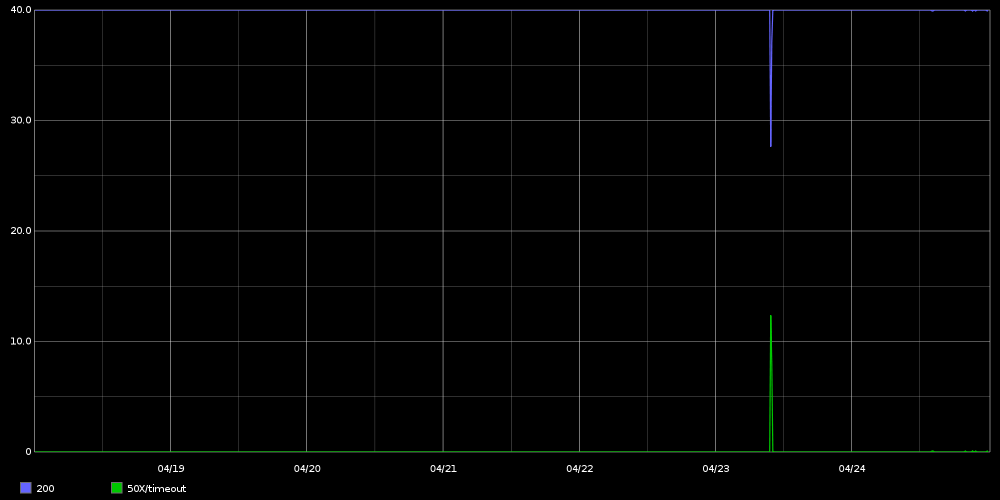
\includegraphics[width=\columnwidth] {images/availability/apr18/threaded_comments_measurer_small.png}}
  \caption{Heartbeat measurement: Summarized HTTP request status codes for each measurement step for application \emph{threaded-comments}}
  \label{fig:heartbeat_tr}
\end{figure}

From the graphs it becomes apparent that when failures occurred, they never affected all instances of a deploy, but only a subset of them. The peak percentages of \emph{down} instances relative to \emph{up} instances are \mytilde6\% for \emph{soundcloud}, \mytilde20\% for \emph{authenticator} and \mytilde57\% for \emph{threaded-comments}. Following this, we define that an application's deploy is \emph{down} in a certain time period, when more than 5\% of all its service instances are \emph{down}.

Table~\ref{tab:heartbeat_failure_probs} shows the results of our measurements as well as the calculated failure probabilities after the equations in \nref{subsec:historical_availability_theory}. As mission time we chose \emph{t = 720 minutes (12hours)}. Using these failure probabilities in the fault tree results in a TOP event probability of \textbf{0,96588}.

\begin{table}[ht]
  \caption{Failure probabilities for application deploys measured via heartbeat measurements from April 18 2014 to April 24 2014 with \emph{down} threshold 5\%. The \emph{mission time} for the failure probability calculation was 720 minutes (12 hours).}
  \label{tab:heartbeat_failure_probs}
  \begin{adjustwidth}{-0.5in}{-.5in}
  \begin{tabular}{ |l|l|l|l|l|l| }
    \hline
    Application & \#Datapoints & \#Up & \#UpSequences & MTTF & Failure probability \\
    \hline
    threaded-comments & 10080 & 10066 & 2 & 5032,50 & 0,1333 \\
    authenticator & 10080 & 10053 & 17 & 591,29 & 0,7040 \\
    soundcloud & 10080 & 9996 & 28 & 356,96 & 0,8669 \\
    \hline
  \end{tabular}
  \end{adjustwidth}
\end{table}

\subsubsection{Discussion}

\emph{Measurer} requested each instance once per time period. We assume that the result of that single request represents the state of the instance for the whole time period. We do not have knowledge about the state of the instance for the rest of the time. Even though this problem could be mitigated by decreasing the measurement interval (for example to one second), it remains a fundamental problem of the method.

For each application we defined one HTTP resource location to query against. Therefore \emph{Measurer} may also only know about the availability of that single resource. Given that an application might show different failure characteristics for different resource locations, the results from our measurement may not capture the complete availability of the instances, as they are experienced by the clients of said instances. Querying more resource locations per instance might mitigate this problem, but its practical applicability is bound to the number of resource locations to query.

During operation the measurements themselves do create load on the instances, thus measuring might alter the results of the measurement. Given that we assume to work with systems that should be able to handle hundreds of requests per second per instance, the effect of measurements should not have a significant impact.
% In our case study execution, this became a problem with the \emph{soundcloud} application, whose service instances handle requests blockingly.

In our investigations we do not guard against network failure. Since we did not experience simultaneous failures of all instances at the same time, we may assume that no total network outage happened during the time of our tests. Still, partial network failures might have altered the results of our measurements.

One of the implicit assumptions we have with this measurement is that our system for executing the measurements experiences no or less failures than the system we measure. This includes \emph{Measurer} as well as \emph{Graphite} (which we used for storing the measurement information). We did not test, as to how much this assumption is true.

Once we had the results from the measurements, we had to decide for each time period if the deploy was \emph{up} or \emph{down}. We based this on a ratio of \emph{up} and \emph{down} instances: if more than 5\% of the instances were \emph{down} we assumed the deploy to be \emph{down}. We set this ratio threshold as a ``good guess'' after manually assessing the collected data. Future work should investigate better ways of assessing the ratio threshold or investigate other ways of making the \emph{up}/\emph{down} assessment for deploys.

\vfill\clearpage

\subsection{Production traffic measurements}
\label{subsec:existing_measurement}

To collect historical availability data of an application deploy, we measured the production traffic for the deploy's service instances. In this section we will explain the method, how we executed it in our case study and discuss our findings.

\subsubsection{Measurement method}

When an application is deployed in the production environment it will serve the production traffic created by the users. Collecting information on that traffic allows us to derive historical availability data.

In our case study we were interested in measuring the three applications \emph{soundcloud}, \emph{authenticator} and \emph{threaded-comments}. All of these have deploys in the production environment. They all use the HTTP~protocol~\cite{rfc2616} to handle requests. For these requests we were able to gather metrics about the returned HTTP status codes from each deploy's service instances. To determine if an application is \emph{up} or \emph{down} for a specific time period we looked at the summed number of requests that returned an HTTP response status code smaller than or equal to \emph{500}. We then set a threshold. If the measured sum was above this threshold we considered the deploy to be \emph{down}.

For measuring the production traffic we used the existing telemetry systems (as outlined earlier in \nref{subsec:telemetry}). Finding the correct telemetry system and metrics within these was a non-trivial task that we executed manually, since it required deep knowledge of the system and measurement architecture. We gathered data for seven days between April 18 2014 and April 24 2014 inclusively.

Next we will explain the exact measurement method for each application deploy and show the respective results:

\paragraph{soundcloud} All traffic to service instances of \emph{soundcloud} goes through \emph{HAProxy}~\cite{haproxy} load balancing servers. The access logs of HAProxy are parsed, aggregated, and saved to \emph{Graphite}. The resolution of the data saved in \emph{Graphite} is 56 minutes. That data is an average of sum per minute over all instances of \emph{HAProxy}. The results can be seen in Figure~\ref{fig:measure_soundcloud}. The \emph{down} threshold was set to 75.

\paragraph{authenticator} Each \emph{authenticator} instance aggregates the HTTP response status codes all requests internally and aggregates them with \emph{Prometheus}. The resolution is 1 minute. The results can be seen in Figure~\ref{fig:measure_auth}. The \emph{down} threshold was set to 20.

\paragraph{threaded-comments} Each \emph{threaded-comments} instance sends the HTTP status code of each response to \emph{statsd}. The resolution is 1 minute. The results can be seen in Figure~\ref{fig:measure_tr}. The \emph{down} threshold was set to 20.

\begin{figure}[ht]
  \fbox{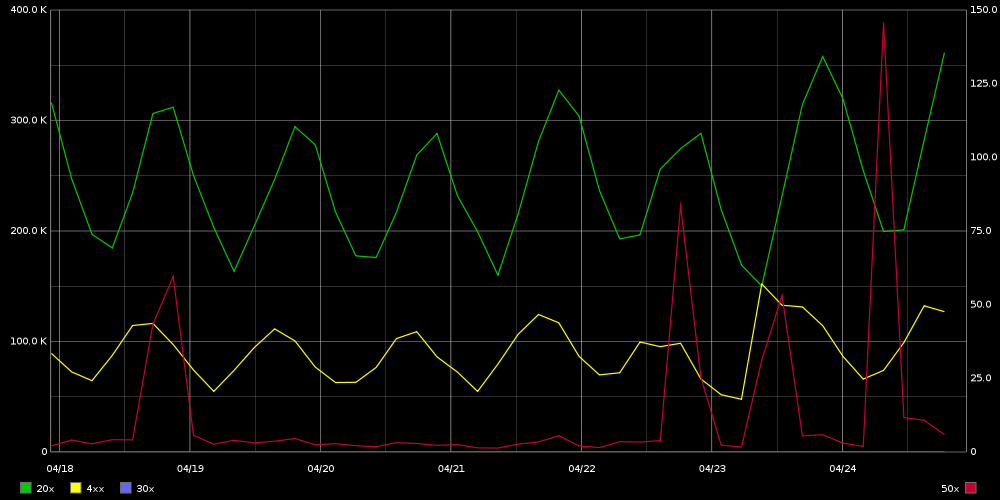
\includegraphics[width=\columnwidth] {images/availability/apr18/soundcloud_haproxy_small.png}}
  \caption{Existing measurements: Summarized HTTP response status codes on \emph{HAProxy} for application \emph{soundcloud}. Please note that there are two y-axes}
  \label{fig:measure_soundcloud}
\end{figure}

\begin{figure}[ht]
  \fbox{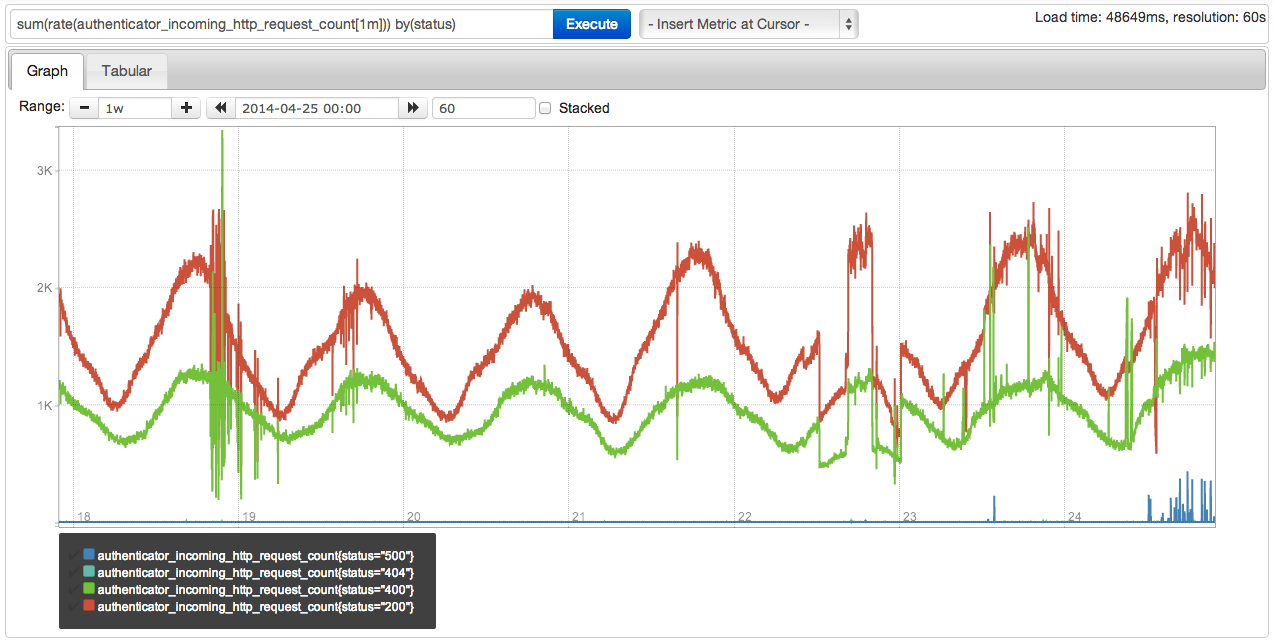
\includegraphics[width=\columnwidth] {images/availability/apr18/authenticator_prometheus_small.png}}
  \caption{Existing measurements: Summarized HTTP response status codes for application \emph{authenticator}}
  \label{fig:measure_auth}
\end{figure}

\begin{figure}[ht]
  \fbox{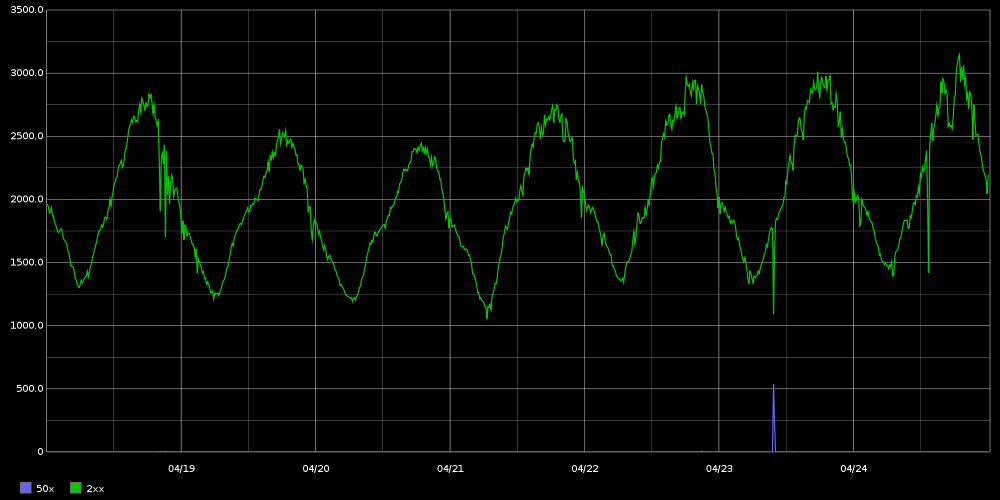
\includegraphics[width=\columnwidth] {images/availability/apr18/threaded_comments_statsd_small.png}}
  \caption{Existing measurements: Summarized HTTP response status codes for application \emph{threaded-comments}}
  \label{fig:measure_tr}
\end{figure}

\subsubsection{Results}

Table~\ref{tab:existing_measure_failure_probs} shows the results of our measurements as well as the calculated failure probabilities after the equations in \nref{subsec:historical_availability_theory}. As mission time we chose \emph{t = 720 minutes (12hours)}. Using these failure probabilities in the fault tree results in a TOP event probability of \textbf{0,96585}.

\begin{table}
  \caption{Failure probabilities for applications measured from production traffic from April 18 2014 to April 24 2014. The \emph{mission time} for the failure probability calculation was 720 minutes (12 hours). Note that we scaled up the datapoints for \emph{soundcloud} to make up for the low granularity provided from the measurement.}
  \label{tab:existing_measure_failure_probs}
  \begin{adjustwidth}{-0.9in}{-.8in}
    \begin{tabular}{ |l|l|l|l|l|l|l|l| }
      \hline
      Application & Threshold & \#Datapoints & \#Ups & \#UpSequences & MTTF & Failure probability \\
      \hline
      soundcloud & 75 & 10080 & 9968 & 3 & 3322,66 & 0,1948 \\
      authenticator & 20 & 10080 & 10037 & 27 & 358,46 & 0,8658 \\
      threaded-comments & 20 & 10080 & 10067 & 2 & 5033,5 & 0,1333 \\
      \hline
    \end{tabular}
  \end{adjustwidth}
\end{table}

\paragraph{Discussion}

In our case study we found two types of how production traffic was measured: \emph{Threaded-comments} and \emph{authenticator} are measured internally, within the instance processes. \emph{Soundcloud} is measured externally, on the load balancer between service consumers and service instances. Both measure the actual service consumer traffic. We believe the external measurements to be more accurate: If a service instance crashes the internal measurement will equally crash and therefore not count failed requests anymore. External measurements can count instance crashes without problems. The assumption with external measurements is then that the complete production traffic is measured on that measuring point. For example in our case study the external measurements happened on the load balancers. We verified that the service instances were not serving production traffic routed through other means. If that would be the case, the other means would have to be incorporated into the external measurements as well.

In our case study the time period resolution of the measurements varied with 56 minutes for \emph{soundcloud} and 1 minute for \emph{threaded-comments} and \emph{authenticator}. This led to an exaggeration of the downtime that we measured for \emph{soundcloud}, which we scaled up to match the resolution of the other measurements. We believe that a high resolution (preferably in the seconds not minutes range) as well as the same resolution for all measurements would improve the quality of the results.

Once we had the results from the measurements, we had to decide for each time period if the deploy was \emph{up} or \emph{down}. We based this on a threshold value of failed responses based on the delivered HTTP status code. We set this threshold as a ``good guess'' after manually assessing the collected data. Future work should investigate better ways of assessing the threshold or investigate other ways of making the \emph{up}/\emph{down}.

\subsection{Discussion}
\label{subsubsec:measure_discussion}

Both approaches measure the perspective of the service consumers and how these experience the service. We believe this to be a good perspective for measuring historical availability since failures are the entity that impedes on a service's availability and failures may only be experienced (and therefore measured) from the service consumer's perspective.

We believe that the \emph{production traffic} approach will deliver more accurate data. We base this opinion on two arguments: The \emph{heartbeat} measurement may only measure a limited number of HTTP resources, whereas the \emph{production traffic} approach will measure all relevant resources, given that these are used by the actual service consumers. Secondly the \emph{heartbeat} approach has the problem of choosing appropriate querying intervals. In the \emph{production traffic} approach, this problem does not exist since the querying intervals are implicitly chosen by the service consumer traffic. If we assume that a service instance serves several hundred requests per second, the effective querying interval in the \emph{production traffic} approach is in the range of milliseconds.

For both approaches we split time into a time series with equal time periods. In both approaches we then had the problem of deciding for each time period, if a deploy as \emph{up} or \emph{down} for that period. In both cases we based this decision on a threshold which we set as a ``good guess''. Depending on the measured data and the chosen threshold value, the resulting \emph{up}/\emph{down} periods may look significantly different. We believe this to be a crucial problem of the methods. Future work should investigate this aspect more.

Next we will compare the resulting MTTFs of both methods in  \autoref{tab:heartbeat_failure_probs} and \autoref{tab:existing_measure_failure_probs}. The MTTFs of \emph{threaded-comments} are nearly the same (\emph{heartbeat}: 5032,50 and \emph{production traffic} 5033,5). The MTTF of the \emph{authenticator} \emph{heartbeat} measurement (591,29) is \mytilde65\% higher than the \emph{production traffic} measurement (358,46). The MTTF of the \emph{soundcloud} \emph{heartbeat measurement} (356,96) is \mytilde10\% of the \emph{production traffic} measurement (3322,66). The lowest MTTFs of both methods are nearly the same (358,46 and 356,96).

\subsubsection{TOP event probability calculation}

Given that we have the historical availability time series for each of the application deploys we need to calculate the failure probability for of them.

First we calculate the MTTF and with that the failure rate. Basis for this calculation is the assumption that the system has reached steady-state. Thus given that our observation period was one week, we assume that all other weeks yield similar MTTF values than the one we observed. This is a weak assumption, since we know from experience that the availability of deploys may differ significantly between weeks. One aspect to investigate for mitigating this effect is observing over longer periods of time.

Based on the failure rate, we may calculate the failure probability. For this we have to assume a failure distribution. We chose the exponential distribution (\autoref{eq:failureprob}) since it allows for analytical calculation. Future work should investigate to which extent it represents failures of application deploys well and if other distributions might be better suited. The exponential distribution equation needs a mission time for calculating the failure probability. We chose 720 minutes as a mission time as a ``good guess''. Intuitively, the higher the mission time, the higher the resulting failure probabilities will be.

Given the failure probabilities for the basic events, we may calculate the TOP event probability of the fault tree. When comparing the two results (\emph{heartbeat approach}: \emph{0,96588} and \emph{production traffic approach}: \emph{0,96585}) we can see that they are very similar, despite the fact that the MTTFs of the individual applications do differ significantly. We attribute the similarity to the fact that the basic event with the highest failure probability has the most significant impact on the calculated TOP event probability. Given that we have seen that the lowest MTTFs of both case study executions is nearly the same, the highest failure probabilities are equally similar, thus leading to similar TOP event probabilities.

One of the assumption when using fault tree basic event probabilities is that they are stochastically independent. When measuring historical availability, this assumption is not necessarily fulfilled, given that applications do depend on each other. We did not investigate this aspect during our measurements. We see opportunity in future work differentiating between ``inherent'' failure and ``propagated'' failure of an application.

\section{Discussion}
\label{sec:quant_discussion}

In this section we will discuss the findings from this chapter, compare the methods we investigated and hint to potential for future work.

In this chapter we have investigated options for creating a quantified fault tree. We based these investigations on the qualitative fault tree constructed in earlier \nref{chapter:fault_trees}. Given such a qualitative fault tree, we may assign failure probabilities to the basic events of the fault tree in order to calculate the TOP event probability. For the fault tree we used in our case study execution, we have shown the equation at the beginning of this chapter in \autoref{eq:quant_prob}.

For obtaining basic event failure probabilities, we investigated four methods: two methods based on \emph{source code metrics} (\nref{sec:source_code}) and two methods based on \emph{historical availability} of application deploys (\nref{sec:historical_availability}). The focus of this work was to investigate the feasibility of the approaches in the context of our case study. We found all approaches to be executable. We did not gather enough information to do a meaningful quantitative analysis, but rather see our work as proof that it is possible to do such analyses.

Comparing the four approaches regarding the numerical values of the TOP event probability is not a fruitful task, since all methods at some point in their execution rely on a threshold or normalization chosen by the user. Still it is possible to qualitatively compare them, which we will do next.

\subsubsection{Mapping application identifiers}

For the methods based on \emph{source code metrics} it was easy to map application identifiers to the respective codebase and source code management repository, since as assumption we earlier established in \nref{sec:software_environment_terminology} that all applications have exactly one codebase with canonical repository location. For \emph{historical availability} this process was a bigger problem. In practice, \emph{historical availability} may only be measured from concrete service instances. The measured values may then be aggregated to represent the deploy, which in turn may be taken as the representation of the application. We were interested in the perspective of applications and dependencies between them since we took that perspective in earlier investigations \nref{chapter:dependency_graph} and \nref{chapter:fault_trees} as well. An opportunity for future work is to use an approach based on service instances. Building the dependency graph and qualitative fault tree might then contribute from our experiences of measuring network traffic as introduced in \nref{subsec:from_network}.

\subsubsection{External applications}

\emph{Lines of code} was the only method with which we calculated probabilities for external applications. We assumed \emph{relative code churn} to not be expressive for external applications, since during our investigations no new versions of the external applications were deployed in our case study. With \emph{historical availability} measurement, we found no representative existing \emph{production traffic measurement} and therefore also did not investigate \emph{external heartbeat measurements} further. Even though we did not execute these methods for external applications in our case study, technically these should be well feasible.

\subsubsection{Source code metrics}

When we executed the \emph{lines of code} method in our case study, it revealed big differences in the size of codebases. Given that we linearly normalized the lines of code to failure probabilities, this led to the over-emphasis of large codebases and the neglectable impact of smaller ones. Future work may investigate, how different mapping functions from \emph{lines of code} to failure probabilities might impact the results.

The calculated \emph{relative code churn} numbers from our case study fluctuated between 0 and \mytilde0,6 depending on the chosen time periods. Also a property of \emph{relative code churn} is that it cumulatively increases with increasing time periods. Fluctuation and cumulation make comparing relative code churn numbers and resulting failure probabilities hard to compare with other methods. Given the assumption that it is a good predictor of failure probabilities, we believe it may be used as an indicator for potential dependability risks. For example application developers could be notified when their service dependency applications show an increase in failure probability based on \emph{relative code churn}.

In our work we only investigated two approaches based on \emph{source code metrics}. Many more exist, which may be investigated in future work. The work by D'Ambros et al \cite{DAmbros2011} surveying defect prediction approaches may provide a good starting point.

\subsubsection{Historical availability}

During our investigation in the case study we found both methods for measuring \emph{historical availability} feasible. We believe that \emph{production traffic measurements} are to be preferred over \emph{heartbeat measurements}, since they test more resources and do not have the problem of choosing an appropriate test interval. We furthermore believe that they are well integrateable in existing measurement systems, thus lowering the complexity for implementation.

One potential problem we noticed, but did not investigate thoroughly, is the difference between ``internal'' and ``propagated'' failures of a service instance. Given that we see that a service instance is unavailable, we do not know if the failure is from within the application itself (``internal'') or cause by another application failing (``propagated''). An opportunity to investigate this in future work is to correlate failures over time, over several systems as well from the users' perspective. We tried to do this in our case study, but during our investigation periods no problems surfaced that allowed for meaningful correlation. In our investigations we therefore assumed all noticed failures to be of ``internal'' nature.

Another interesting opportunity for future work is the decomposition of services into separate resources or functionalities. Each may then be measured individually for its availability. This would allow for more fine-grained fault trees and failure correlations, which would allow more detailed insights into the architecture.

\subsubsection{Reliability for repairable systems}

In the way we used fault trees here, the TOP event probability denotes the unreliability of the investigated system, without taking repairs into consideration. We believe software always to be repairable (most fundamentally by restarting it). Future work might investigate how to reflect this property in fault tree investigation.

\subsubsection{Duplicated basic events}

In the fault tree we used (\autoref{fig:fault_tree_threaded_comments}) there are no duplicate basic events. Our method for calculating the TOP event probability requires all basic event to be stochastically independent. This can be a problem, since there is no guarantee that in the methods we introduced. In practice, once two separate applications (\emph{A} and \emph{B}) depend on the same other application (\emph{C}), then that application \emph{C} will be represented twice in the resulting fault tree. Examples can be seen in \autoref{fig:fault_tree_v2}, where the basic event ``5'' exists many times.

\subsubsection{Investigate change}

Our investigations with \emph{code churn} are the only ones that allow for looking at changes of the resulting TOP event probability over time. We see potential in further investigating this with the other methods, especially how changes to an application do impact the TOP event probability. Looking at changes over time would also allow for comparing the results of the methods better, since it would be possible to correlate changes.

\section{Summary}

In this chapter we investigated approaches to constructing a quantitative fault tree. Given a qualitative fault tree the TOP event probability may be calculated if basic event probabilities exist. We investigated two types of methods for gathering basic event probabilities for applications: source code metrics and historical availability. The two source code metrics \emph{lines of code} and \emph{relative code churn} are known to allow prediction of defects. We proposed to extend these metrics for calculating failure probabilities. Similarly, \emph{historical availability measurements} allow the calculation basic event probabilities. We proved the feasibility of these methods by executing them in our case study and gathered promising results, but more work is needed to quantifiably evaluate these.
  %!TEX root = ../master_thesis.tex

\chapter{Discussion}
\label{chapter:discussion}

One of the starting points of this work was using fault trees as a way to model the dependability of microservice architectures. As a step towards constructing fault trees for a deployed microservice architecture, we investigated dependency graphs on the granularity level of applications and their service dependencies. During that process we learned that the dependency graphs themselves already are valuable tools in modeling the structure of a deployed architecture, since they allow engineers to answer the questions ``Which applications does my application depend on?'' and ``Which applications depend on my application?''. They even provide that visibility transitively over multiple degrees of service dependencies. In comparison, the qualitative fault trees we constructed were not better suited for visually assessing an architecture, due to their significantly larger size.

However, the structure of qualitative fault trees allowed us to construct quantitative fault trees for calculating TOP event probabilities. In this work we showed that it is possible to construct them, however the resulting TOP event probabilities were only a first step towards a wide range of opportunities for assessing dependability attributes. We especially see two fields of interest for future work: Quantitative fault trees may help to quantify the impact of changes to an architecture and therefore inform architectural and engineering decisions. They may also be valuable tools for aggregating realtime measurements when operating a microservice architecture.

One of the enabling factors in our investigations was the existence of infrastructure systems, which lead to a ``programmable infrastructure''. Due to their distributed nature, microservice architectures suffer from a distribution of meta information about the system. Gathering information about a deployed and running microservice architecture therefore requires dedicated infrastructure systems that collect, instrument, store and provide this meta information. These infrastructure systems are needed to allow automated investigations like the ones presented in this work.

This thesis is a first step towards researching the benefits of modeling dependability through dependencies in microservice architectures. To reduce the complexity of the work in this thesis, we excluded fault tolerance from investigations. We believe that including fault tolerance into the modeling approaches is a logical next step. This might aid representing reality better in the models and improve their expressiveness.
  %!TEX root = ../master_thesis.tex

\chapter{Summary}
\label{chapter:summary}
% Motivation
In this work we showed approaches for modeling dependability in microservice architectures and applied these in a case study with the ``Software as a Service" company ``SoundCloud''. When building a software system in the microservice architectural style, engineers face the problem of assessing its dependability attributes. In a microservice architecture many individual applications work together as one software system. These applications depend on each other, which leads to the possibility of failures propagating through the system.

%What did you do

In this thesis we assessed to what extend dependency graphs and fault trees could be used to model dependability of microservice architectures. As a basis we proposed our own terminology model for describing microservice architectures. Based on that model, we constructed dependency graphs, transformed them automatically to qualitative fault trees and investigated quantifying the fault trees with failure probabilities.

% How did it go?

In our investigations, we found dependency graphs to be a valuable tool for visualizing applications and their dependencies in microservice architectures. Dependency graphs turned out to be a better visualization of service dependencies than qualitative fault trees, due to their significantly smaller size. For constructing dependency graphs from a deployed microservice architecture we investigated four methods. Our qualitative evaluation did not reveal a clear preference for a specific method, but we see three of them (\emph{semi-automatic creation from manual annotations}, \emph{from deployment configuration}, \emph{from network traffic}) as viable methods.

We believe quantitative fault trees may be used for assessing the impact of architectural change on the dependability of applications in microservice architectures. In this thesis we have proven the possibility to construct them for a deployed microservice architecture. We showed four possible ways for gathering failure probabilities for applications. We found the methods of \emph{relative code churn} and \emph{historical availability from production traffic} to be promising.

All methods we described were executed in the context of the case study with ``SoundCloud'' and therefore have been tested with real data in a productively deployed microservice architecture.

We believe that there is a tendency to utilize the microservice architectural style, since it allows for building big and complex software systems by dividing and encapsulating business concerns into individual services. Furthermore it has proven in the industry to be a viable way of constructing ``Software as a Service" systems. Therefore we believe the microservice architectural style to grow in importance in the future. With that the problem of assessing dependability of such an architecture is raised. In this work we specifically addressed the problem of low visibility for dependencies between applications. We believe that this improves the discussion of dependability in microservice architectures, but many more subjects of that discussion remain open for further investigation. We look forward to the future work in industry and academia on these topics.

\scalebox{.02}{Zweifel. Conquered at last.}
  % %!TEX root = ../master_thesis.tex

\chapter{Notes}

This chapter includes notes by johan and removed parts.

\todo{Remove this chapter before publishing}

\section{General Todos}

CNAME? is that even used correctly?

Rechtschreibkontrolle (copy paste pdf text in google docs?)

Zeitplan:

\begin{tabular}{ |l|l| }
  \hline
  Dienstag & Check das die ganzen Bibliographies nett aussehen. Jeweils \emph{namen et al} dran bitte \\
  Dienstag & Check das alle tables/figures label nach der caption haben \\
  Mittwoch & Finales layout schauen (wo ist die grafik? wo ist die tabelle?) \\
  Mittwoch & Nochmal komplett durchlesen, drucken, abgeben \\

  \hline
  x & Mehr code churn? \\
  x & Three-tier architecture \\
  x & \nref{subsec:fault_tree_construction} \nref{sec:case_study_execution} semantic vertice names? \\
  x & tree pruning schon eher im algorithmus machen? \\
  x & Tool chain for alle dependency models erklären. Vielleicht nur generell, wie ich den graph generiert habe? Kleine Tools, Go, Instrumentiert via Bash, Input/Processing/Output \\

  \hline
  Dienstag & Doppel/mehrfachleerzeichen?\\
  Dienstag & Alle wörter von unten consistency suchen und jeweils korrigieren \\
  Dienstag & Latex fehler beseitigen. gibt es einen ``strict'' mode?\\
  Dienstag & Suche nach todos in code and check that nothing is left \\
  Dienstag & Check das alle referenzen da sind (nach ? suchen) \\
\end{tabular}

\section{Consistency}

Consistency with emphasize:
\begin{tabular}{ |l|l| }
  \hline
 ``keyword'' & literal quotation from somewhere \\
  \emph{keyword} & introducing a special word from elsewhere \\
  \textbf{keyword} & highlighting special words describing this section \\
  \hline
\end{tabular}

Words to use:
\begin{tabular}{ |l|l| }
  \hline
  Yes & No \\
  \hline
  case study & use case \\
  case study & soundcloud \\
  time series & timeseries \\
  investigation & experiment \\
  codebase & code base \\
  vertices | vertex &  nodes | node \\
  subgraph & sub graph \\
  plotted graph & graph (because a graph is a data structure)\\
  method | mechanism | procedure & process \\
  case study = vergangenheit & present \\
  we & me/i \\
  Go & go \\
  HAProxy & haproxy \\
  MySQL & mysql \\
  RabbitMQ & rabbitmq \\
  internal.example.com & int.s-cloud.net \\
  reverse service discovery & inverse service discovery \\
  people & humans \\
  applications & components \\
  quantitative/qualitative & quantitive/qualitive \\
  service dependency & application dependency (plural)\\
  heartbeat & hearbeat \\
  external & vendor \\
  tenumerate & enumerate \\
  itemize & titemize \\
  description & tdescription \\
  configuration | deployment environment & environment \\
  \hline
\end{tabular}

\chapter{Removed parts TODO:REMOVE}

\section{Structure from application deploys}

Assume fault tree from previous section \nref{section:fault_tree_structure}.

Based on number of process instances. Therefore based on deploys of application, with instances of procs.

\todo{No idea how this works, have to collaborate with troeger}

\subsection{Software structure}

\todo{Do i actually want to have this in here? markdown has much}

\todo{I feel this point needs to be in here, because I want to make sure to show that there is a difference between "architecture at runtime" and "architecture from code". but maybe these are better words to use, instead of structure. So I might want to abandon "Software Structure" alltogether?}

\subsection{Service interface}

\definition{A service interface is the abstract boundary that a service exposes to its service consumers.}

Abstract thing, but can be described via a service defintion language.

\todo{copy from markdown}

\subsection{Service consumer}

\definition{A service consumer is a program, that communicates with a service to send requests.}

A program might be any code, that can be executed in a runtime. In our context, a program will usually exist in the context of an application.

\todo{copy definiton from markdown}


\section{case study}
A note of caution: the nature of engineering in a company like SoundCloud is built around the principle of being able to evolve the products quickly~\footnote{ "Move fast and break things" from Facebook}. Therefore, the implementation details as outlined here are likely to have changed already.

Some cases where several applications per repository. Since they still host the application itself in that repository, we will ignore that case for now, but each time treat whole repository as being code base for that application.

\section{faul trees}
\subsubsection{Transformation rules}

Given that we have a fault tree, we may transform it to an equation of boolean logic. \autoref{tab:fault_tree_bool} shows the transformation rules.

\begin{table}[ht]
  \caption{Transformation rules: Fault tree to boolean logic}
  \label{tab:fault_tree_bool}
  \begin{tabular}{ |l|l| }
    \hline
    Fault tree & Boolean logic \\
    \hline
    TOP Event & Result of equation \\
    Basic Event & Operand \\
    Intermediate Event & Connected elements enclosed in parentheses \\
    OR-Gate & Operator \(\vee\) between connected events \\
    AND-Gate & Opeator \(\wedge\) between connected events \\
    \hline
  \end{tabular}
\end{table}

Given the boolean logic equation, we may transform it to an equation with statistical probabilities to calculate the failure probability of the top event. The rules are shown in \autoref{tab:bool_prob}.

\begin{table}[ht]
  \caption{Transformation rules: Boolean logic to statistical probabilities}
  \label{tab:bool_prob}
  \begin{tabular}{ |l|l| }
    \hline
    Boolean logic & Statstical probabilities \\
    \hline
    Operand \emph{A} & Probability of failure \emph{P(A)} \\
    \(A \wedge B\) & \(P(A \wedge B) = P(A \cap B) = P(A)P(B)\) \\
    \(A \vee B\) & \(P(A \vee B) = P(A \cup B) = P(A) + P(B) -  P(A \cap B)\) \\
    \hline
  \end{tabular}
\end{table}

An example of these transformations can be seen in  \nref{chap:quantitive_fault_tree}.

\subsection{Circular dependencies}
\label{section:circular_dependencies}

\definition{A circular dependency between application A and application B exists, if A has a service dependency on B and B has a service dependency on A.}

\todo{picture of this}

Circular dependencies might also be transitive, thus via another application.

Circular dependencies are usually regarded as bad style \todo{citation needed}. In our case, they make it impossible to generate a fault tree, since by definition a tree does not allow circular dependencies.

Still, in our case study we have seen circular dependencies happening.
Mothership. Depends on analytics microservice. Analytics microservice has ETL job that needs to query the mothership for master data. Different processes but still everything within one application \todo{move the concrete info somewhere else, and only say: We discuss this subject more in ...}

  % BIBLIOGRAPHY
  \cleardoublepage
  \renewcommand{\bibname}{References}
  \renewcommand{\refname}{References}
  \addcontentsline{toc}{chapter}{References}
  \printbibliography
  % end BIBLIOGRAPHY
\end{document}
